\documentclass[twoside]{book}

% Packages required by doxygen
\usepackage{fixltx2e}
\usepackage{calc}
\usepackage{doxygen}
\usepackage[export]{adjustbox} % also loads graphicx
\usepackage{graphicx}
\usepackage[utf8]{inputenc}
\usepackage{makeidx}
\usepackage{multicol}
\usepackage{multirow}
\PassOptionsToPackage{warn}{textcomp}
\usepackage{textcomp}
\usepackage[nointegrals]{wasysym}
\usepackage[table]{xcolor}

% Font selection
\usepackage[T1]{fontenc}
\usepackage[scaled=.90]{helvet}
\usepackage{courier}
\usepackage{amssymb}
\usepackage{sectsty}
\renewcommand{\familydefault}{\sfdefault}
\allsectionsfont{%
  \fontseries{bc}\selectfont%
  \color{darkgray}%
}
\renewcommand{\DoxyLabelFont}{%
  \fontseries{bc}\selectfont%
  \color{darkgray}%
}
\newcommand{\+}{\discretionary{\mbox{\scriptsize$\hookleftarrow$}}{}{}}

% Page & text layout
\usepackage{geometry}
\geometry{%
  a4paper,%
  top=2.5cm,%
  bottom=2.5cm,%
  left=2.5cm,%
  right=2.5cm%
}
\tolerance=750
\hfuzz=15pt
\hbadness=750
\setlength{\emergencystretch}{15pt}
\setlength{\parindent}{0cm}
\setlength{\parskip}{0.2cm}
\makeatletter
\renewcommand{\paragraph}{%
  \@startsection{paragraph}{4}{0ex}{-1.0ex}{1.0ex}{%
    \normalfont\normalsize\bfseries\SS@parafont%
  }%
}
\renewcommand{\subparagraph}{%
  \@startsection{subparagraph}{5}{0ex}{-1.0ex}{1.0ex}{%
    \normalfont\normalsize\bfseries\SS@subparafont%
  }%
}
\makeatother

% Headers & footers
\usepackage{fancyhdr}
\pagestyle{fancyplain}
\fancyhead[LE]{\fancyplain{}{\bfseries\thepage}}
\fancyhead[CE]{\fancyplain{}{}}
\fancyhead[RE]{\fancyplain{}{\bfseries\leftmark}}
\fancyhead[LO]{\fancyplain{}{\bfseries\rightmark}}
\fancyhead[CO]{\fancyplain{}{}}
\fancyhead[RO]{\fancyplain{}{\bfseries\thepage}}
\fancyfoot[LE]{\fancyplain{}{}}
\fancyfoot[CE]{\fancyplain{}{}}
\fancyfoot[RE]{\fancyplain{}{\bfseries\scriptsize Generated on Thu May 14 2015 21\+:20\+:54 for Irrigation test system 1 by Doxygen }}
\fancyfoot[LO]{\fancyplain{}{\bfseries\scriptsize Generated on Thu May 14 2015 21\+:20\+:54 for Irrigation test system 1 by Doxygen }}
\fancyfoot[CO]{\fancyplain{}{}}
\fancyfoot[RO]{\fancyplain{}{}}
\renewcommand{\footrulewidth}{0.4pt}
\renewcommand{\chaptermark}[1]{%
  \markboth{#1}{}%
}
\renewcommand{\sectionmark}[1]{%
  \markright{\thesection\ #1}%
}

% Indices & bibliography
\usepackage{natbib}
\usepackage[titles]{tocloft}
\setcounter{tocdepth}{3}
\setcounter{secnumdepth}{5}
\makeindex

% Hyperlinks (required, but should be loaded last)
\usepackage{ifpdf}
\ifpdf
  \usepackage[pdftex,pagebackref=true]{hyperref}
\else
  \usepackage[ps2pdf,pagebackref=true]{hyperref}
\fi
\hypersetup{%
  colorlinks=true,%
  linkcolor=blue,%
  citecolor=blue,%
  unicode%
}

% Custom commands
\newcommand{\clearemptydoublepage}{%
  \newpage{\pagestyle{empty}\cleardoublepage}%
}


%===== C O N T E N T S =====

\begin{document}

% Titlepage & ToC
\hypersetup{pageanchor=false,
             bookmarks=true,
             bookmarksnumbered=true,
             pdfencoding=unicode
            }
\pagenumbering{roman}
\begin{titlepage}
\vspace*{7cm}
\begin{center}%
{\Large Irrigation test system 1 }\\
\vspace*{1cm}
{\large Generated by Doxygen 1.8.9.1}\\
\vspace*{0.5cm}
{\small Thu May 14 2015 21:20:54}\\
\end{center}
\end{titlepage}
\clearemptydoublepage
\tableofcontents
\clearemptydoublepage
\pagenumbering{arabic}
\hypersetup{pageanchor=true}

%--- Begin generated contents ---
\chapter{Irrigation Controller}
\label{index}\hypertarget{index}{}\hypertarget{index_index_sec}{}\section{Index}\label{index_index_sec}
\begin{DoxyItemize}
\item \hyperlink{main_8c}{main.\+c} Main file \end{DoxyItemize}

\chapter{Todo List}
\label{todo}
\hypertarget{todo}{}

\begin{DoxyRefList}
\item[\label{todo__todo000001}%
\hypertarget{todo__todo000001}{}%
File \hyperlink{hw_8h}{hw.h} ]There is some stuff not belonging to this file in here, it should be moved 
\item[\label{todo__todo000002}%
\hypertarget{todo__todo000002}{}%
global\+Scope$>$ Member \hyperlink{hw_8h_a3c02952100e7d051b77cdf060ca0ba9ba45012c00c17031e71a4f60ada04df07d}{H\+W\+\_\+\+I\+N\+I\+T\+\_\+\+P\+R\+E\+\_\+\+N\+V\+I\+C} ]Implement the default value thing  
\item[\label{todo__todo000004}%
\hypertarget{todo__todo000004}{}%
Member \hyperlink{structirrigation__controller__status_ab795e232c4e2d405b11e24312a6163c3}{irrigation\+\_\+controller\+\_\+status\+:\+:last\+\_\+hot\+\_\+sample} ]Clean up unused stuff here  
\item[\label{todo__todo000005}%
\hypertarget{todo__todo000005}{}%
File \hyperlink{main_8c}{main.c} ]systick, adc, moisture sensor, pwm output, filter 

explain port and rcc better 
\item[\label{todo__todo000003}%
\hypertarget{todo__todo000003}{}%
global\+Scope$>$ Member \hyperlink{irrigation_8h_a9891f6b3b37611d2aebdb8601acdf6c6a4460d045ceb966a377b72d2825606fbd}{moisture\+\_\+sensor\+\_\+t1} ]t1 and t2 are not used for the moment  
\item[\label{todo__todo000006}%
\hypertarget{todo__todo000006}{}%
global\+Scope$>$ Member \hyperlink{timer_8h_a995539ac62815c22bad2313f304865b5}{timer\+\_\+ccr\+\_\+init} (struct \hyperlink{structtimer__ccr}{timer\+\_\+ccr} $\ast$ccr, enum hw\+\_\+init\+\_\+state state)]Add more C\+C\+R-\/channels 

Only upgrade state if needed  
\item[\label{todo__todo000008}%
\hypertarget{todo__todo000008}{}%
global\+Scope$>$ Member \hyperlink{usart_8c_a0e3103fc345dfb09aa255989c86805e8}{usart\+\_\+init} (struct usart $\ast$usart, enum hw\+\_\+init\+\_\+state state)]Check if we are inited already 
\end{DoxyRefList}
\chapter{Module Index}
\section{Modules}
Here is a list of all modules\+:\begin{DoxyCompactList}
\item \contentsline{section}{Initial state}{\pageref{group__state__init}}{}
\item \contentsline{section}{Sensor validation state}{\pageref{group__state__validate}}{}
\item \contentsline{section}{Reboot state}{\pageref{group__state__reboot}}{}
\item \contentsline{section}{This state makes the actual soil measure}{\pageref{group__state__measure}}{}
\end{DoxyCompactList}

\chapter{Class Index}
\section{Class List}
Here are the classes, structs, unions and interfaces with brief descriptions\+:\begin{DoxyCompactList}
\item\contentsline{section}{\hyperlink{structadc}{adc} }{\pageref{structadc}}{}
\item\contentsline{section}{\hyperlink{structadc__config}{adc\+\_\+config} }{\pageref{structadc__config}}{}
\item\contentsline{section}{\hyperlink{structdma__channel__config}{dma\+\_\+channel\+\_\+config} }{\pageref{structdma__channel__config}}{}
\item\contentsline{section}{\hyperlink{structdma__config}{dma\+\_\+config} }{\pageref{structdma__config}}{}
\item\contentsline{section}{\hyperlink{structfilter__rms}{filter\+\_\+rms} \\*R\+M\+S filter configuration and state }{\pageref{structfilter__rms}}{}
\item\contentsline{section}{\hyperlink{structfilter__sample__range}{filter\+\_\+sample\+\_\+range} \\*A valid range for samples }{\pageref{structfilter__sample__range}}{}
\item\contentsline{section}{\hyperlink{structgpio__pin}{gpio\+\_\+pin} }{\pageref{structgpio__pin}}{}
\item\contentsline{section}{\hyperlink{structgpio__pin__config}{gpio\+\_\+pin\+\_\+config} }{\pageref{structgpio__pin__config}}{}
\item\contentsline{section}{\hyperlink{structgpio__port}{gpio\+\_\+port} }{\pageref{structgpio__port}}{}
\item\contentsline{section}{\hyperlink{structgpio__port__config}{gpio\+\_\+port\+\_\+config} }{\pageref{structgpio__port__config}}{}
\item\contentsline{section}{\hyperlink{structirrigation__controller}{irrigation\+\_\+controller} \\*Holds everything related to the irrigation controller }{\pageref{structirrigation__controller}}{}
\item\contentsline{section}{\hyperlink{structirrigation__controller__status}{irrigation\+\_\+controller\+\_\+status} }{\pageref{structirrigation__controller__status}}{}
\item\contentsline{section}{\hyperlink{structirrigation__events}{irrigation\+\_\+events} \\*The event callback functions for the irrigation controller core }{\pageref{structirrigation__events}}{}
\item\contentsline{section}{\hyperlink{structirrigation__temperature__sample}{irrigation\+\_\+temperature\+\_\+sample} \\*This is a timestamped temperature sample }{\pageref{structirrigation__temperature__sample}}{}
\item\contentsline{section}{\hyperlink{structsw__timer__system__time}{sw\+\_\+timer\+\_\+system\+\_\+time} \\*Timestamp }{\pageref{structsw__timer__system__time}}{}
\item\contentsline{section}{\hyperlink{structsystick}{systick} }{\pageref{structsystick}}{}
\item\contentsline{section}{\hyperlink{structsystick__config}{systick\+\_\+config} }{\pageref{structsystick__config}}{}
\item\contentsline{section}{\hyperlink{structtimer}{timer} }{\pageref{structtimer}}{}
\item\contentsline{section}{\hyperlink{structtimer__ccr}{timer\+\_\+ccr} }{\pageref{structtimer__ccr}}{}
\item\contentsline{section}{\hyperlink{structtimer__ccr__config}{timer\+\_\+ccr\+\_\+config} }{\pageref{structtimer__ccr__config}}{}
\item\contentsline{section}{\hyperlink{structtimer__config}{timer\+\_\+config} }{\pageref{structtimer__config}}{}
\item\contentsline{section}{\hyperlink{structtm}{tm} \\*Broken down time }{\pageref{structtm}}{}
\item\contentsline{section}{\hyperlink{structusart}{usart} \\*Usart }{\pageref{structusart}}{}
\item\contentsline{section}{\hyperlink{structusart__config}{usart\+\_\+config} \\*Usart configuration }{\pageref{structusart__config}}{}
\item\contentsline{section}{\hyperlink{structws2812}{ws2812} \\*W\+S2812 Instance }{\pageref{structws2812}}{}
\item\contentsline{section}{\hyperlink{structws2812__config}{ws2812\+\_\+config} \\*Configuration for W\+S2812 }{\pageref{structws2812__config}}{}
\item\contentsline{section}{\hyperlink{structws2812__rgb}{ws2812\+\_\+rgb} \\*24 bit color }{\pageref{structws2812__rgb}}{}
\end{DoxyCompactList}

\chapter{File Index}
\section{File List}
Here is a list of all documented files with brief descriptions\+:\begin{DoxyCompactList}
\item\contentsline{section}{src/\hyperlink{adc_8c}{adc.\+c} \\*A\+D\+C H\+A\+L implementation }{\pageref{adc_8c}}{}
\item\contentsline{section}{src/\hyperlink{adc_8h}{adc.\+h} \\*A\+D\+C H\+A\+L include }{\pageref{adc_8h}}{}
\item\contentsline{section}{src/\hyperlink{dma_8c}{dma.\+c} \\*D\+M\+A implementation }{\pageref{dma_8c}}{}
\item\contentsline{section}{src/\hyperlink{dma_8h}{dma.\+h} \\*D\+M\+A includes }{\pageref{dma_8h}}{}
\item\contentsline{section}{src/{\bfseries dma\+\_\+macro.\+h} }{\pageref{dma__macro_8h}}{}
\item\contentsline{section}{src/\hyperlink{filter_8c}{filter.\+c} \\*Implementation of filter functions }{\pageref{filter_8c}}{}
\item\contentsline{section}{src/\hyperlink{filter_8h}{filter.\+h} \\*Filter functions for filtering sensor data }{\pageref{filter_8h}}{}
\item\contentsline{section}{src/\hyperlink{gpio_8c}{gpio.\+c} \\*G\+P\+I\+O H\+A\+L implementation }{\pageref{gpio_8c}}{}
\item\contentsline{section}{src/\hyperlink{gpio_8h}{gpio.\+h} \\*G\+P\+I\+O H\+A\+L includes }{\pageref{gpio_8h}}{}
\item\contentsline{section}{src/\hyperlink{gpio__macro_8h}{gpio\+\_\+macro.\+h} \\*Helper macros for G\+P\+I\+O }{\pageref{gpio__macro_8h}}{}
\item\contentsline{section}{src/\hyperlink{hw_8c}{hw.\+c} \\*H\+A\+L main control }{\pageref{hw_8c}}{}
\item\contentsline{section}{src/\hyperlink{hw_8h}{hw.\+h} \\*Hardware abstraction layer include file }{\pageref{hw_8h}}{}
\item\contentsline{section}{src/\hyperlink{irrigation_8h}{irrigation.\+h} \\*Irrigation main include file }{\pageref{irrigation_8h}}{}
\item\contentsline{section}{src/\hyperlink{led__macro_8h}{led\+\_\+macro.\+h} \\*Helper macros for L\+E\+D control }{\pageref{led__macro_8h}}{}
\item\contentsline{section}{src/\hyperlink{main_8c}{main.\+c} \\*Irrigation controller main file }{\pageref{main_8c}}{}
\item\contentsline{section}{src/\hyperlink{math_8h}{math.\+h} \\*Some math utilities }{\pageref{math_8h}}{}
\item\contentsline{section}{src/\hyperlink{state__init_8c}{state\+\_\+init.\+c} \\*Initial state }{\pageref{state__init_8c}}{}
\item\contentsline{section}{src/\hyperlink{state__measure_8c}{state\+\_\+measure.\+c} \\*Measurement state }{\pageref{state__measure_8c}}{}
\item\contentsline{section}{src/\hyperlink{state__reboot_8c}{state\+\_\+reboot.\+c} \\*Rebooting state }{\pageref{state__reboot_8c}}{}
\item\contentsline{section}{src/\hyperlink{state__validate_8c}{state\+\_\+validate.\+c} \\*Sensor validation state }{\pageref{state__validate_8c}}{}
\item\contentsline{section}{src/\hyperlink{systick_8c}{systick.\+c} \\*Systick H\+A\+L implementation }{\pageref{systick_8c}}{}
\item\contentsline{section}{src/\hyperlink{systick_8h}{systick.\+h} \\*Systick H\+A\+L include }{\pageref{systick_8h}}{}
\item\contentsline{section}{src/{\bfseries systick\+\_\+macro.\+h} }{\pageref{systick__macro_8h}}{}
\item\contentsline{section}{src/\hyperlink{time_8c}{time.\+c} \\*Time keeping and conversation functions }{\pageref{time_8c}}{}
\item\contentsline{section}{src/\hyperlink{time_8h}{time.\+h} \\*Time keeping and converting include file }{\pageref{time_8h}}{}
\item\contentsline{section}{src/\hyperlink{timer_8c}{timer.\+c} \\*Timer H\+A\+L implementation }{\pageref{timer_8c}}{}
\item\contentsline{section}{src/\hyperlink{timer_8h}{timer.\+h} \\*Timer H\+A\+L include file }{\pageref{timer_8h}}{}
\item\contentsline{section}{src/\hyperlink{timer__macro_8h}{timer\+\_\+macro.\+h} \\*Utility macros for timers }{\pageref{timer__macro_8h}}{}
\item\contentsline{section}{src/\hyperlink{uart_8h}{uart.\+h} \\*U\+A\+R\+T H\+A\+L Include file }{\pageref{uart_8h}}{}
\item\contentsline{section}{src/\hyperlink{usart_8c}{usart.\+c} \\*U\+S\+A\+R\+T H\+A\+L driver }{\pageref{usart_8c}}{}
\item\contentsline{section}{src/\hyperlink{usart__macro_8h}{usart\+\_\+macro.\+h} \\*Helper macros for U\+S\+A\+R\+T }{\pageref{usart__macro_8h}}{}
\item\contentsline{section}{src/\hyperlink{ws2812_8c}{ws2812.\+c} \\*Implementation of W\+S2812 H\+A\+L }{\pageref{ws2812_8c}}{}
\item\contentsline{section}{src/\hyperlink{ws2812_8h}{ws2812.\+h} \\*W\+S2812 H\+A\+L include file }{\pageref{ws2812_8h}}{}
\item\contentsline{section}{src/\hyperlink{ws2812__macro_8h}{ws2812\+\_\+macro.\+h} \\*Helper macros for \hyperlink{structws2812}{ws2812} }{\pageref{ws2812__macro_8h}}{}
\end{DoxyCompactList}

\chapter{Module Documentation}
\hypertarget{group__state__init}{}\section{Initial state}
\label{group__state__init}\index{Initial state@{Initial state}}
\subsection*{Functions}
\begin{DoxyCompactItemize}
\item 
void \hyperlink{group__state__init_gaeca2f683660bf42f5258acd6aac353d0}{state\+\_\+init\+\_\+enter} (struct \hyperlink{structirrigation__controller}{irrigation\+\_\+controller} $\ast$controller)
\begin{DoxyCompactList}\small\item\em Reset all variables in the controller this state uses. \end{DoxyCompactList}\item 
void \hyperlink{group__state__init_ga5b5f5a7ec8534a643fb599efdee6ed4f}{state\+\_\+init\+\_\+run} (struct \hyperlink{structirrigation__controller}{irrigation\+\_\+controller} $\ast$controller)
\begin{DoxyCompactList}\small\item\em We will make a heart beat ramp for the status L\+E\+D while we wait for initial delay to complete. \end{DoxyCompactList}\item 
void \hyperlink{group__state__init_ga52863e306edb45d15c12acdecb7e5555}{state\+\_\+init\+\_\+exit} (struct \hyperlink{structirrigation__controller}{irrigation\+\_\+controller} $\ast$controller)
\begin{DoxyCompactList}\small\item\em Nothing has do be done before we leave this state. \end{DoxyCompactList}\end{DoxyCompactItemize}


\subsection{Detailed Description}


\subsection{Function Documentation}
\hypertarget{group__state__init_gaeca2f683660bf42f5258acd6aac353d0}{}\index{Initial state@{Initial state}!state\+\_\+init\+\_\+enter@{state\+\_\+init\+\_\+enter}}
\index{state\+\_\+init\+\_\+enter@{state\+\_\+init\+\_\+enter}!Initial state@{Initial state}}
\subsubsection[{state\+\_\+init\+\_\+enter}]{\setlength{\rightskip}{0pt plus 5cm}void state\+\_\+init\+\_\+enter (
\begin{DoxyParamCaption}
\item[{struct {\bf irrigation\+\_\+controller} $\ast$}]{controller}
\end{DoxyParamCaption}
)}\label{group__state__init_gaeca2f683660bf42f5258acd6aac353d0}


Reset all variables in the controller this state uses. 



Definition at line 8 of file state\+\_\+init.\+c.



References irrigation\+\_\+controller\+\_\+status\+::initial\+\_\+timer, and irrigation\+\_\+controller\+::status.

\hypertarget{group__state__init_ga52863e306edb45d15c12acdecb7e5555}{}\index{Initial state@{Initial state}!state\+\_\+init\+\_\+exit@{state\+\_\+init\+\_\+exit}}
\index{state\+\_\+init\+\_\+exit@{state\+\_\+init\+\_\+exit}!Initial state@{Initial state}}
\subsubsection[{state\+\_\+init\+\_\+exit}]{\setlength{\rightskip}{0pt plus 5cm}void state\+\_\+init\+\_\+exit (
\begin{DoxyParamCaption}
\item[{struct {\bf irrigation\+\_\+controller} $\ast$}]{controller}
\end{DoxyParamCaption}
)}\label{group__state__init_ga52863e306edb45d15c12acdecb7e5555}


Nothing has do be done before we leave this state. 



Definition at line 38 of file state\+\_\+init.\+c.

\hypertarget{group__state__init_ga5b5f5a7ec8534a643fb599efdee6ed4f}{}\index{Initial state@{Initial state}!state\+\_\+init\+\_\+run@{state\+\_\+init\+\_\+run}}
\index{state\+\_\+init\+\_\+run@{state\+\_\+init\+\_\+run}!Initial state@{Initial state}}
\subsubsection[{state\+\_\+init\+\_\+run}]{\setlength{\rightskip}{0pt plus 5cm}void state\+\_\+init\+\_\+run (
\begin{DoxyParamCaption}
\item[{struct {\bf irrigation\+\_\+controller} $\ast$}]{controller}
\end{DoxyParamCaption}
)}\label{group__state__init_ga5b5f5a7ec8534a643fb599efdee6ed4f}


We will make a heart beat ramp for the status L\+E\+D while we wait for initial delay to complete. 



Definition at line 14 of file state\+\_\+init.\+c.



References irrigation\+\_\+controller\+\_\+status\+::dt, irrigation\+\_\+controller\+\_\+status\+::initial\+\_\+timer, irrigation\+\_\+status\+\_\+\+V\+A\+L\+I\+D\+A\+T\+E, math\+\_\+ramp, irrigation\+\_\+controller\+::pending\+\_\+state, and irrigation\+\_\+controller\+::status.


\hypertarget{group__state__validate}{}\section{Sensor validation state}
\label{group__state__validate}\index{Sensor validation state@{Sensor validation state}}
\subsection*{Functions}
\begin{DoxyCompactItemize}
\item 
void \hyperlink{group__state__validate_gac0d41d4685bd461b3a613f6320405b79}{state\+\_\+validate\+\_\+enter} (struct \hyperlink{structirrigation__controller}{irrigation\+\_\+controller} $\ast$controller)
\begin{DoxyCompactList}\small\item\em We set up the validation timer and init the maximum and minim temperatured. \end{DoxyCompactList}\item 
void \hyperlink{group__state__validate_gaec38509b93f8a850919aa7a36e543ed5}{state\+\_\+validate\+\_\+run} (struct \hyperlink{structirrigation__controller}{irrigation\+\_\+controller} $\ast$controller)
\begin{DoxyCompactList}\small\item\em We have the heart beat L\+E\+D status and we update the minimum and maximum values while we continue to sample sensor data. \end{DoxyCompactList}\item 
void \hyperlink{group__state__validate_gac480e756742ffd9acd9bd21ac1e8885c}{state\+\_\+validate\+\_\+exit} (struct \hyperlink{structirrigation__controller}{irrigation\+\_\+controller} $\ast$controller)
\begin{DoxyCompactList}\small\item\em Nothing has to be done when we exit this state. \end{DoxyCompactList}\end{DoxyCompactItemize}


\subsection{Detailed Description}


\subsection{Function Documentation}
\hypertarget{group__state__validate_gac0d41d4685bd461b3a613f6320405b79}{}\index{Sensor validation state@{Sensor validation state}!state\+\_\+validate\+\_\+enter@{state\+\_\+validate\+\_\+enter}}
\index{state\+\_\+validate\+\_\+enter@{state\+\_\+validate\+\_\+enter}!Sensor validation state@{Sensor validation state}}
\subsubsection[{state\+\_\+validate\+\_\+enter}]{\setlength{\rightskip}{0pt plus 5cm}void state\+\_\+validate\+\_\+enter (
\begin{DoxyParamCaption}
\item[{struct {\bf irrigation\+\_\+controller} $\ast$}]{controller}
\end{DoxyParamCaption}
)}\label{group__state__validate_gac0d41d4685bd461b3a613f6320405b79}


We set up the validation timer and init the maximum and minim temperatured. 

We also check that we have current sensor data availble 

Definition at line 10 of file state\+\_\+validate.\+c.



References irrigation\+\_\+status\+\_\+\+R\+E\+B\+O\+O\+T, irrigation\+\_\+controller\+\_\+status\+::iteration\+\_\+time, irrigation\+\_\+controller\+\_\+status\+::max\+\_\+temperature, irrigation\+\_\+controller\+\_\+status\+::min\+\_\+temperature, irrigation\+\_\+controller\+::pending\+\_\+state, irrigation\+\_\+events\+::report\+\_\+sensor\+\_\+malfunction, irrigation\+\_\+controller\+\_\+status\+::soil\+\_\+temperature, irrigation\+\_\+controller\+::status, irrigation\+\_\+temperature\+\_\+sample\+::temperature, time\+\_\+delta, irrigation\+\_\+temperature\+\_\+sample\+::timestamp, and irrigation\+\_\+controller\+\_\+status\+::validation\+\_\+timer.

\hypertarget{group__state__validate_gac480e756742ffd9acd9bd21ac1e8885c}{}\index{Sensor validation state@{Sensor validation state}!state\+\_\+validate\+\_\+exit@{state\+\_\+validate\+\_\+exit}}
\index{state\+\_\+validate\+\_\+exit@{state\+\_\+validate\+\_\+exit}!Sensor validation state@{Sensor validation state}}
\subsubsection[{state\+\_\+validate\+\_\+exit}]{\setlength{\rightskip}{0pt plus 5cm}void state\+\_\+validate\+\_\+exit (
\begin{DoxyParamCaption}
\item[{struct {\bf irrigation\+\_\+controller} $\ast$}]{controller}
\end{DoxyParamCaption}
)}\label{group__state__validate_gac480e756742ffd9acd9bd21ac1e8885c}


Nothing has to be done when we exit this state. 



Definition at line 66 of file state\+\_\+validate.\+c.

\hypertarget{group__state__validate_gaec38509b93f8a850919aa7a36e543ed5}{}\index{Sensor validation state@{Sensor validation state}!state\+\_\+validate\+\_\+run@{state\+\_\+validate\+\_\+run}}
\index{state\+\_\+validate\+\_\+run@{state\+\_\+validate\+\_\+run}!Sensor validation state@{Sensor validation state}}
\subsubsection[{state\+\_\+validate\+\_\+run}]{\setlength{\rightskip}{0pt plus 5cm}void state\+\_\+validate\+\_\+run (
\begin{DoxyParamCaption}
\item[{struct {\bf irrigation\+\_\+controller} $\ast$}]{controller}
\end{DoxyParamCaption}
)}\label{group__state__validate_gaec38509b93f8a850919aa7a36e543ed5}


We have the heart beat L\+E\+D status and we update the minimum and maximum values while we continue to sample sensor data. 

When timeout is reached we verify that the sensor data span is reasonable 

Definition at line 26 of file state\+\_\+validate.\+c.



References irrigation\+\_\+controller\+\_\+status\+::dt, irrigation\+\_\+status\+\_\+\+M\+E\+A\+S\+U\+R\+E, irrigation\+\_\+status\+\_\+\+R\+E\+B\+O\+O\+T, irrigation\+\_\+controller\+\_\+status\+::iteration\+\_\+time, math\+\_\+ramp, M\+A\+X, irrigation\+\_\+controller\+\_\+status\+::max\+\_\+temperature, M\+I\+N, irrigation\+\_\+controller\+\_\+status\+::min\+\_\+temperature, irrigation\+\_\+controller\+::pending\+\_\+state, irrigation\+\_\+events\+::report\+\_\+sensor\+\_\+fluctuations, irrigation\+\_\+events\+::report\+\_\+sensor\+\_\+malfunction, irrigation\+\_\+events\+::report\+\_\+validation\+\_\+temperatures, irrigation\+\_\+controller\+\_\+status\+::soil\+\_\+temperature, irrigation\+\_\+controller\+::status, irrigation\+\_\+temperature\+\_\+sample\+::temperature, time\+\_\+delta, irrigation\+\_\+temperature\+\_\+sample\+::timestamp, and irrigation\+\_\+controller\+\_\+status\+::validation\+\_\+timer.


\hypertarget{group__state__reboot}{}\section{Reboot state}
\label{group__state__reboot}\index{Reboot state@{Reboot state}}


This state makes sure the systems exits in a nice way before it starts up again.  


\subsection*{Functions}
\begin{DoxyCompactItemize}
\item 
\hypertarget{group__state__reboot_gab0e3409fa69ff96792cb5a768928a545}{}void {\bfseries state\+\_\+reboot\+\_\+enter} (struct \hyperlink{structirrigation__controller}{irrigation\+\_\+controller} $\ast$controller)\label{group__state__reboot_gab0e3409fa69ff96792cb5a768928a545}

\item 
\hypertarget{group__state__reboot_ga23cf1ecfb670c7c6c253a40705aa5caf}{}void {\bfseries state\+\_\+reboot\+\_\+run} (struct \hyperlink{structirrigation__controller}{irrigation\+\_\+controller} $\ast$controller)\label{group__state__reboot_ga23cf1ecfb670c7c6c253a40705aa5caf}

\item 
\hypertarget{group__state__reboot_gafbcdeb4b017f4350fb6ff51df410228b}{}void {\bfseries state\+\_\+reboot\+\_\+exit} (struct \hyperlink{structirrigation__controller}{irrigation\+\_\+controller} $\ast$controller)\label{group__state__reboot_gafbcdeb4b017f4350fb6ff51df410228b}

\end{DoxyCompactItemize}


\subsection{Detailed Description}
This state makes sure the systems exits in a nice way before it starts up again. 


\hypertarget{group__state__measure}{}\section{This state makes the actual soil measure}
\label{group__state__measure}\index{This state makes the actual soil measure@{This state makes the actual soil measure}}
\subsection*{Functions}
\begin{DoxyCompactItemize}
\item 
void \hyperlink{group__state__measure_ga24a42892ba25be220bff68fc151e0be7}{state\+\_\+measure\+\_\+enter} (struct \hyperlink{structirrigation__controller}{irrigation\+\_\+controller} $\ast$controller)
\begin{DoxyCompactList}\small\item\em Measure state enter. \end{DoxyCompactList}\item 
\hypertarget{group__state__measure_ga410776694bde81bde92a0b6b178ac015}{}void {\bfseries state\+\_\+measure\+\_\+run} (struct \hyperlink{structirrigation__controller}{irrigation\+\_\+controller} $\ast$controller)\label{group__state__measure_ga410776694bde81bde92a0b6b178ac015}

\item 
\hypertarget{group__state__measure_ga0f85f8645f5311e776e85a3697517266}{}void {\bfseries state\+\_\+measure\+\_\+exit} (struct \hyperlink{structirrigation__controller}{irrigation\+\_\+controller} $\ast$controller)\label{group__state__measure_ga0f85f8645f5311e776e85a3697517266}

\end{DoxyCompactItemize}


\subsection{Detailed Description}


\subsection{Function Documentation}
\hypertarget{group__state__measure_ga24a42892ba25be220bff68fc151e0be7}{}\index{This state makes the actual soil measure@{This state makes the actual soil measure}!state\+\_\+measure\+\_\+enter@{state\+\_\+measure\+\_\+enter}}
\index{state\+\_\+measure\+\_\+enter@{state\+\_\+measure\+\_\+enter}!This state makes the actual soil measure@{This state makes the actual soil measure}}
\subsubsection[{state\+\_\+measure\+\_\+enter}]{\setlength{\rightskip}{0pt plus 5cm}void state\+\_\+measure\+\_\+enter (
\begin{DoxyParamCaption}
\item[{struct {\bf irrigation\+\_\+controller} $\ast$}]{controller}
\end{DoxyParamCaption}
)}\label{group__state__measure_ga24a42892ba25be220bff68fc151e0be7}


Measure state enter. 

The following things are done in this function \begin{DoxyItemize}
\item It is asserted that the last soil temperature is no older than 10 m\+S\end{DoxyItemize}
\begin{DoxyItemize}
\item last\+\_\+soil\+\_\+sample is set to soil\+\_\+temperature\end{DoxyItemize}
\begin{DoxyItemize}
\item Initializing variables used in run state\end{DoxyItemize}
\begin{DoxyItemize}
\item Report that heater was started \end{DoxyItemize}


Definition at line 12 of file state\+\_\+measure.\+c.



References irrigation\+\_\+status\+\_\+\+R\+E\+B\+O\+O\+T, irrigation\+\_\+controller\+\_\+status\+::iteration\+\_\+time, irrigation\+\_\+controller\+\_\+status\+::last\+\_\+soil\+\_\+sample, moisture\+\_\+sensor\+\_\+heating, irrigation\+\_\+controller\+::pending\+\_\+state, irrigation\+\_\+controller\+\_\+status\+::periodic\+\_\+temp\+\_\+report, irrigation\+\_\+events\+::report\+\_\+msg\+\_\+note, irrigation\+\_\+events\+::report\+\_\+sensor\+\_\+malfunction, irrigation\+\_\+controller\+\_\+status\+::soil\+\_\+temperature, irrigation\+\_\+controller\+::status, time\+\_\+delta, and irrigation\+\_\+temperature\+\_\+sample\+::timestamp.


\chapter{Class Documentation}
\hypertarget{structadc}{}\section{adc Struct Reference}
\label{structadc}\index{adc@{adc}}


Collaboration diagram for adc\+:\nopagebreak
\begin{figure}[H]
\begin{center}
\leavevmode
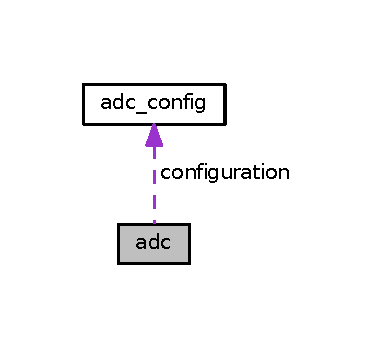
\includegraphics[width=180pt]{structadc__coll__graph}
\end{center}
\end{figure}
\subsection*{Public Attributes}
\begin{DoxyCompactItemize}
\item 
\hypertarget{structadc_aaecb8053d6389a045fd2fd05b3b2f584}{}struct \hyperlink{structadc__config}{adc\+\_\+config} $\ast$ {\bfseries configuration}\label{structadc_aaecb8053d6389a045fd2fd05b3b2f584}

\item 
\hypertarget{structadc_a18f6e4c34b612060add403c39b12c44a}{}uint16\+\_\+t $\ast$ {\bfseries adc\+\_\+buffer}\label{structadc_a18f6e4c34b612060add403c39b12c44a}

\item 
\hypertarget{structadc_a83e9b544b8780ab70e5c193a4b5d8ef8}{}bool {\bfseries sampling\+\_\+done}\label{structadc_a83e9b544b8780ab70e5c193a4b5d8ef8}

\end{DoxyCompactItemize}


\subsection{Detailed Description}


Definition at line 17 of file adc.\+h.



The documentation for this struct was generated from the following file\+:\begin{DoxyCompactItemize}
\item 
src/\hyperlink{adc_8h}{adc.\+h}\end{DoxyCompactItemize}

\hypertarget{structadc__config}{}\section{adc\+\_\+config Struct Reference}
\label{structadc__config}\index{adc\+\_\+config@{adc\+\_\+config}}
\subsection*{Public Attributes}
\begin{DoxyCompactItemize}
\item 
\hypertarget{structadc__config_a7f7cc3ba237533dd943faddca7555430}{}uint8\+\_\+t $\ast$ {\bfseries channel\+\_\+map}\label{structadc__config_a7f7cc3ba237533dd943faddca7555430}

\item 
\hypertarget{structadc__config_a33bd54712a72f2dcbd6c3d6d53b776ea}{}int {\bfseries channel\+\_\+count}\label{structadc__config_a33bd54712a72f2dcbd6c3d6d53b776ea}

\end{DoxyCompactItemize}


\subsection{Detailed Description}


Definition at line 12 of file adc.\+h.



The documentation for this struct was generated from the following file\+:\begin{DoxyCompactItemize}
\item 
src/\hyperlink{adc_8h}{adc.\+h}\end{DoxyCompactItemize}

\hypertarget{structdma__channel__config}{}\section{dma\+\_\+channel\+\_\+config Struct Reference}
\label{structdma__channel__config}\index{dma\+\_\+channel\+\_\+config@{dma\+\_\+channel\+\_\+config}}


Collaboration diagram for dma\+\_\+channel\+\_\+config\+:\nopagebreak
\begin{figure}[H]
\begin{center}
\leavevmode
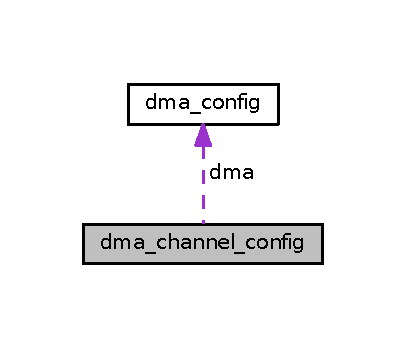
\includegraphics[width=195pt]{structdma__channel__config__coll__graph}
\end{center}
\end{figure}
\subsection*{Public Attributes}
\begin{DoxyCompactItemize}
\item 
\hypertarget{structdma__channel__config_a0352048b957404e734bae6df7678ad38}{}struct \hyperlink{structdma__config}{dma\+\_\+config} $\ast$ {\bfseries dma}\label{structdma__channel__config_a0352048b957404e734bae6df7678ad38}

\item 
\hypertarget{structdma__channel__config_a924e6ca6c88d830241be32248294b63e}{}uint32\+\_\+t {\bfseries channel}\label{structdma__channel__config_a924e6ca6c88d830241be32248294b63e}

\item 
\hypertarget{structdma__channel__config_a1502b9f3fb49ee8e7a04ff49ff07e7c1}{}volatile uint32\+\_\+t $\ast$ {\bfseries perhipheral}\label{structdma__channel__config_a1502b9f3fb49ee8e7a04ff49ff07e7c1}

\item 
\hypertarget{structdma__channel__config_ae5a311bdf13af6200280be76472b60a0}{}volatile uint32\+\_\+t $\ast$ {\bfseries enable\+\_\+reg}\label{structdma__channel__config_ae5a311bdf13af6200280be76472b60a0}

\item 
\hypertarget{structdma__channel__config_ab58f12489030ee869dcf457eabf80cd6}{}uint32\+\_\+t {\bfseries enable\+\_\+flag}\label{structdma__channel__config_ab58f12489030ee869dcf457eabf80cd6}

\end{DoxyCompactItemize}


\subsection{Detailed Description}


Definition at line 17 of file dma.\+h.



The documentation for this struct was generated from the following file\+:\begin{DoxyCompactItemize}
\item 
src/\hyperlink{dma_8h}{dma.\+h}\end{DoxyCompactItemize}

\hypertarget{structdma__config}{}\section{dma\+\_\+config Struct Reference}
\label{structdma__config}\index{dma\+\_\+config@{dma\+\_\+config}}
\subsection*{Public Attributes}
\begin{DoxyCompactItemize}
\item 
\hypertarget{structdma__config_a5a2895e50c0d073d7dc48e4cdee05b1d}{}uint32\+\_\+t {\bfseries dma}\label{structdma__config_a5a2895e50c0d073d7dc48e4cdee05b1d}

\item 
\hypertarget{structdma__config_aba8fd7114a6b26ab99e67c1b7bb8dd4e}{}uint32\+\_\+t {\bfseries rcc}\label{structdma__config_aba8fd7114a6b26ab99e67c1b7bb8dd4e}

\end{DoxyCompactItemize}


\subsection{Detailed Description}


Definition at line 12 of file dma.\+h.



The documentation for this struct was generated from the following file\+:\begin{DoxyCompactItemize}
\item 
src/\hyperlink{dma_8h}{dma.\+h}\end{DoxyCompactItemize}

\hypertarget{structfilter__rms}{}\section{filter\+\_\+rms Struct Reference}
\label{structfilter__rms}\index{filter\+\_\+rms@{filter\+\_\+rms}}


R\+M\+S filter configuration and state.  




{\ttfamily \#include $<$filter.\+h$>$}



Collaboration diagram for filter\+\_\+rms\+:\nopagebreak
\begin{figure}[H]
\begin{center}
\leavevmode
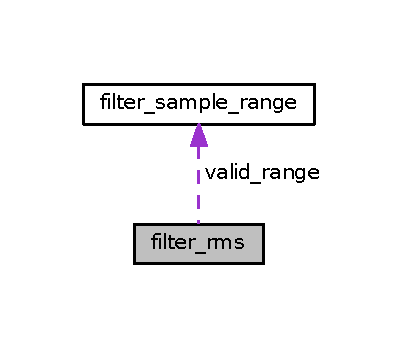
\includegraphics[width=194pt]{structfilter__rms__coll__graph}
\end{center}
\end{figure}
\subsection*{Public Attributes}
\begin{DoxyCompactItemize}
\item 
\hypertarget{structfilter__rms_a54520c4d0cb0f9441f4c57eacf5bfd78}{}volatile uint32\+\_\+t $\ast$ {\bfseries buffer}\label{structfilter__rms_a54520c4d0cb0f9441f4c57eacf5bfd78}

\item 
\hypertarget{structfilter__rms_a8581be35641ea200e6bf23ce48f76196}{}uint32\+\_\+t {\bfseries size}\label{structfilter__rms_a8581be35641ea200e6bf23ce48f76196}

\item 
\hypertarget{structfilter__rms_a85d467406ed373c2ad1a134860fd24bd}{}int {\bfseries pos}\label{structfilter__rms_a85d467406ed373c2ad1a134860fd24bd}

\item 
\hypertarget{structfilter__rms_a42976cc476c577216f312bcd496eb79b}{}uint32\+\_\+t {\bfseries count}\label{structfilter__rms_a42976cc476c577216f312bcd496eb79b}

\item 
\hypertarget{structfilter__rms_a902e6aa671bf468ba0506ef5848f51cf}{}uint32\+\_\+t {\bfseries sqsum}\label{structfilter__rms_a902e6aa671bf468ba0506ef5848f51cf}

\item 
\hypertarget{structfilter__rms_a00a96dc7cf61e9c2643fdefc3d558ff2}{}int {\bfseries invalid\+\_\+samples\+\_\+streak}\label{structfilter__rms_a00a96dc7cf61e9c2643fdefc3d558ff2}

\item 
\hypertarget{structfilter__rms_abcd2a21aa49c2abb148493265da1efa5}{}struct \hyperlink{structfilter__sample__range}{filter\+\_\+sample\+\_\+range} {\bfseries valid\+\_\+range}\label{structfilter__rms_abcd2a21aa49c2abb148493265da1efa5}

\end{DoxyCompactItemize}


\subsection{Detailed Description}
R\+M\+S filter configuration and state. 

Definition at line 15 of file filter.\+h.



The documentation for this struct was generated from the following file\+:\begin{DoxyCompactItemize}
\item 
src/\hyperlink{filter_8h}{filter.\+h}\end{DoxyCompactItemize}

\hypertarget{structfilter__sample__range}{}\section{filter\+\_\+sample\+\_\+range Struct Reference}
\label{structfilter__sample__range}\index{filter\+\_\+sample\+\_\+range@{filter\+\_\+sample\+\_\+range}}


A valid range for samples.  




{\ttfamily \#include $<$filter.\+h$>$}

\subsection*{Public Attributes}
\begin{DoxyCompactItemize}
\item 
\hypertarget{structfilter__sample__range_a304ee67b1a15b4a0f36ca190a56a38c7}{}int {\bfseries min}\label{structfilter__sample__range_a304ee67b1a15b4a0f36ca190a56a38c7}

\item 
\hypertarget{structfilter__sample__range_a0a29f8303981c999d499070d0a05e05d}{}int {\bfseries max}\label{structfilter__sample__range_a0a29f8303981c999d499070d0a05e05d}

\end{DoxyCompactItemize}


\subsection{Detailed Description}
A valid range for samples. 

Definition at line 9 of file filter.\+h.



The documentation for this struct was generated from the following file\+:\begin{DoxyCompactItemize}
\item 
src/\hyperlink{filter_8h}{filter.\+h}\end{DoxyCompactItemize}

\hypertarget{structgpio__pin}{}\section{gpio\+\_\+pin Struct Reference}
\label{structgpio__pin}\index{gpio\+\_\+pin@{gpio\+\_\+pin}}


Collaboration diagram for gpio\+\_\+pin\+:\nopagebreak
\begin{figure}[H]
\begin{center}
\leavevmode
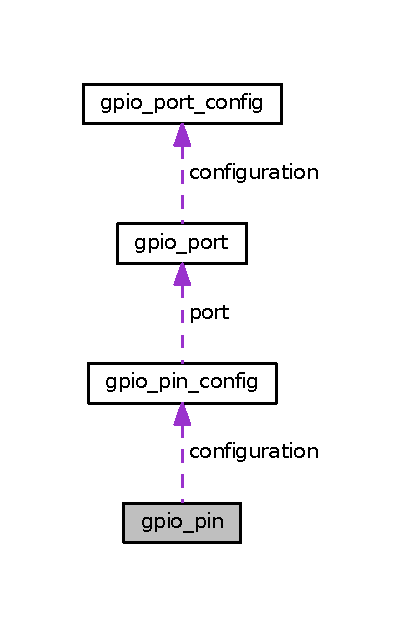
\includegraphics[width=194pt]{structgpio__pin__coll__graph}
\end{center}
\end{figure}
\subsection*{Public Attributes}
\begin{DoxyCompactItemize}
\item 
\hypertarget{structgpio__pin_acb6a2426999aa0f3e40d37a02f791e75}{}struct \hyperlink{structgpio__pin__config}{gpio\+\_\+pin\+\_\+config} $\ast$ {\bfseries configuration}\label{structgpio__pin_acb6a2426999aa0f3e40d37a02f791e75}

\item 
\hypertarget{structgpio__pin_a4d4c7f491d051331985524f88f81fa58}{}enum \hyperlink{hw_8h_a3c02952100e7d051b77cdf060ca0ba9b}{hw\+\_\+init\+\_\+state} {\bfseries state}\label{structgpio__pin_a4d4c7f491d051331985524f88f81fa58}

\end{DoxyCompactItemize}


\subsection{Detailed Description}


Definition at line 29 of file gpio.\+h.



The documentation for this struct was generated from the following file\+:\begin{DoxyCompactItemize}
\item 
src/\hyperlink{gpio_8h}{gpio.\+h}\end{DoxyCompactItemize}

\hypertarget{structgpio__pin__config}{}\section{gpio\+\_\+pin\+\_\+config Struct Reference}
\label{structgpio__pin__config}\index{gpio\+\_\+pin\+\_\+config@{gpio\+\_\+pin\+\_\+config}}


Collaboration diagram for gpio\+\_\+pin\+\_\+config\+:\nopagebreak
\begin{figure}[H]
\begin{center}
\leavevmode
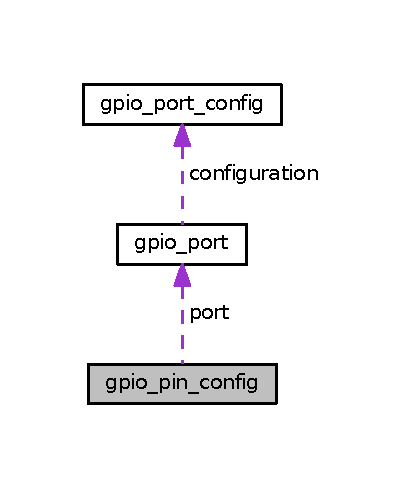
\includegraphics[width=194pt]{structgpio__pin__config__coll__graph}
\end{center}
\end{figure}
\subsection*{Public Attributes}
\begin{DoxyCompactItemize}
\item 
\hypertarget{structgpio__pin__config_a72fc1227f3fab0d1e2485d8f4bed6dbc}{}struct \hyperlink{structgpio__port}{gpio\+\_\+port} $\ast$ {\bfseries port}\label{structgpio__pin__config_a72fc1227f3fab0d1e2485d8f4bed6dbc}

\item 
\hypertarget{structgpio__pin__config_afb9b5bbf5c85e22120e7ef67964b621a}{}uint32\+\_\+t {\bfseries pin}\label{structgpio__pin__config_afb9b5bbf5c85e22120e7ef67964b621a}

\item 
\hypertarget{structgpio__pin__config_a799cc96abd94ffdc23f888a9ed1556ca}{}uint32\+\_\+t {\bfseries mode}\label{structgpio__pin__config_a799cc96abd94ffdc23f888a9ed1556ca}

\item 
\hypertarget{structgpio__pin__config_a1ba8ae193e2164dd8c4238c81d9200e4}{}uint32\+\_\+t {\bfseries configuration}\label{structgpio__pin__config_a1ba8ae193e2164dd8c4238c81d9200e4}

\item 
\hypertarget{structgpio__pin__config_a195076654c4665c2dae2702f4bce5dfd}{}int {\bfseries initial}\label{structgpio__pin__config_a195076654c4665c2dae2702f4bce5dfd}

\end{DoxyCompactItemize}


\subsection{Detailed Description}


Definition at line 21 of file gpio.\+h.



The documentation for this struct was generated from the following file\+:\begin{DoxyCompactItemize}
\item 
src/\hyperlink{gpio_8h}{gpio.\+h}\end{DoxyCompactItemize}

\hypertarget{structgpio__port}{}\section{gpio\+\_\+port Struct Reference}
\label{structgpio__port}\index{gpio\+\_\+port@{gpio\+\_\+port}}


Collaboration diagram for gpio\+\_\+port\+:\nopagebreak
\begin{figure}[H]
\begin{center}
\leavevmode
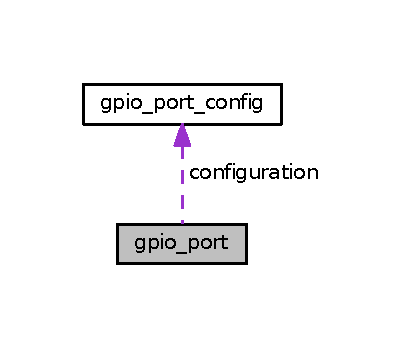
\includegraphics[width=194pt]{structgpio__port__coll__graph}
\end{center}
\end{figure}
\subsection*{Public Attributes}
\begin{DoxyCompactItemize}
\item 
\hypertarget{structgpio__port_ad67106287ff2c5d84c528b731374d5e8}{}struct \hyperlink{structgpio__port__config}{gpio\+\_\+port\+\_\+config} $\ast$ {\bfseries configuration}\label{structgpio__port_ad67106287ff2c5d84c528b731374d5e8}

\item 
\hypertarget{structgpio__port_acc0ba075ca33d19af55b06b16edd7ac6}{}enum \hyperlink{hw_8h_a3c02952100e7d051b77cdf060ca0ba9b}{hw\+\_\+init\+\_\+state} {\bfseries state}\label{structgpio__port_acc0ba075ca33d19af55b06b16edd7ac6}

\end{DoxyCompactItemize}


\subsection{Detailed Description}


Definition at line 11 of file gpio.\+h.



The documentation for this struct was generated from the following file\+:\begin{DoxyCompactItemize}
\item 
src/\hyperlink{gpio_8h}{gpio.\+h}\end{DoxyCompactItemize}

\hypertarget{structgpio__port__config}{}\section{gpio\+\_\+port\+\_\+config Struct Reference}
\label{structgpio__port__config}\index{gpio\+\_\+port\+\_\+config@{gpio\+\_\+port\+\_\+config}}
\subsection*{Public Attributes}
\begin{DoxyCompactItemize}
\item 
\hypertarget{structgpio__port__config_a37f5f40d14a183161a8dd4fd9ede9d05}{}uint32\+\_\+t {\bfseries port}\label{structgpio__port__config_a37f5f40d14a183161a8dd4fd9ede9d05}

\item 
\hypertarget{structgpio__port__config_a00cb058b3750f38e4b3c5be01e9b0f25}{}uint32\+\_\+t {\bfseries rcc}\label{structgpio__port__config_a00cb058b3750f38e4b3c5be01e9b0f25}

\end{DoxyCompactItemize}


\subsection{Detailed Description}


Definition at line 16 of file gpio.\+h.



The documentation for this struct was generated from the following file\+:\begin{DoxyCompactItemize}
\item 
src/\hyperlink{gpio_8h}{gpio.\+h}\end{DoxyCompactItemize}

\hypertarget{structirrigation__controller}{}\section{irrigation\+\_\+controller Struct Reference}
\label{structirrigation__controller}\index{irrigation\+\_\+controller@{irrigation\+\_\+controller}}


Holds everything related to the irrigation controller.  




{\ttfamily \#include $<$irrigation.\+h$>$}



Collaboration diagram for irrigation\+\_\+controller\+:\nopagebreak
\begin{figure}[H]
\begin{center}
\leavevmode
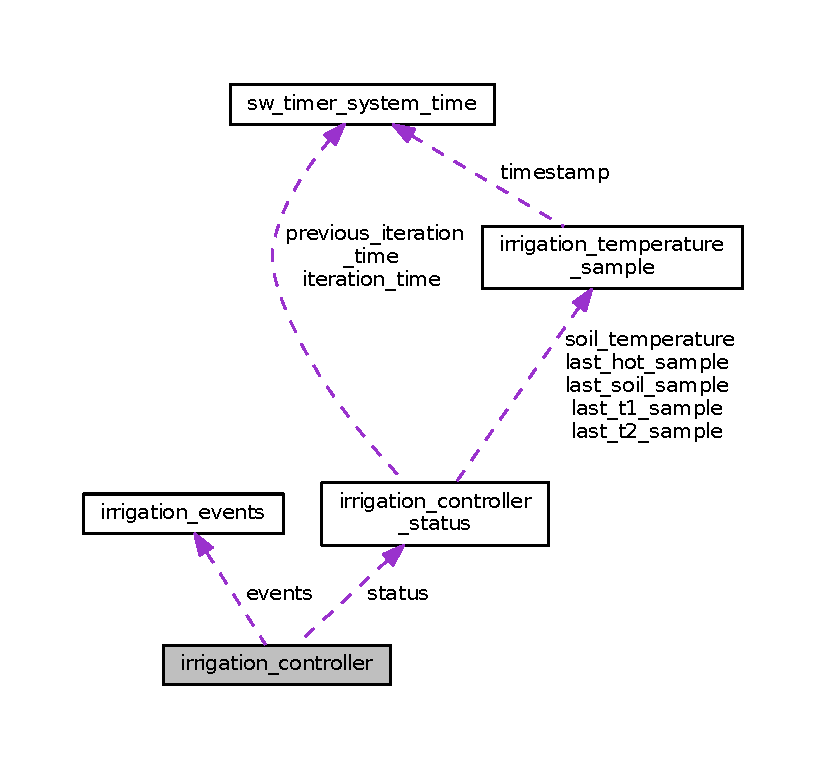
\includegraphics[width=350pt]{structirrigation__controller__coll__graph}
\end{center}
\end{figure}
\subsection*{Public Attributes}
\begin{DoxyCompactItemize}
\item 
struct \hyperlink{structirrigation__controller__status}{irrigation\+\_\+controller\+\_\+status} \hyperlink{structirrigation__controller_a68a854df15c9234d24f2ad36b990bfa8}{status}
\begin{DoxyCompactList}\small\item\em Status and measurements. \end{DoxyCompactList}\item 
enum \hyperlink{irrigation_8h_ac40bd72ec6942e213e454ebcacc92dc7}{irrigation\+\_\+status} \hyperlink{structirrigation__controller_a80bec16de2d6f98564ed1487dee041c5}{current\+\_\+state}
\begin{DoxyCompactList}\small\item\em Current state in the state\+\_\+machine. \end{DoxyCompactList}\item 
enum \hyperlink{irrigation_8h_ac40bd72ec6942e213e454ebcacc92dc7}{irrigation\+\_\+status} \hyperlink{structirrigation__controller_a7e1c5689983d2b8aae434c2d5442c935}{pending\+\_\+state}
\begin{DoxyCompactList}\small\item\em Pending state in the state\+\_\+machine. \end{DoxyCompactList}\item 
\hypertarget{structirrigation__controller_a4ae62413005c2121bee0ac25a0119cbc}{}struct \hyperlink{structirrigation__events}{irrigation\+\_\+events} {\bfseries events}\label{structirrigation__controller_a4ae62413005c2121bee0ac25a0119cbc}

\item 
\hypertarget{structirrigation__controller_a94cb4b4c26de9f40543f06335afa036c}{}int {\bfseries heater}\label{structirrigation__controller_a94cb4b4c26de9f40543f06335afa036c}

\item 
\hypertarget{structirrigation__controller_a38217da0082898392465f4ee2901f73b}{}int {\bfseries pump}\label{structirrigation__controller_a38217da0082898392465f4ee2901f73b}

\end{DoxyCompactItemize}


\subsection{Detailed Description}
Holds everything related to the irrigation controller. 

Definition at line 83 of file irrigation.\+h.



\subsection{Member Data Documentation}
\hypertarget{structirrigation__controller_a80bec16de2d6f98564ed1487dee041c5}{}\index{irrigation\+\_\+controller@{irrigation\+\_\+controller}!current\+\_\+state@{current\+\_\+state}}
\index{current\+\_\+state@{current\+\_\+state}!irrigation\+\_\+controller@{irrigation\+\_\+controller}}
\subsubsection[{current\+\_\+state}]{\setlength{\rightskip}{0pt plus 5cm}enum {\bf irrigation\+\_\+status} irrigation\+\_\+controller\+::current\+\_\+state}\label{structirrigation__controller_a80bec16de2d6f98564ed1487dee041c5}


Current state in the state\+\_\+machine. 



Definition at line 85 of file irrigation.\+h.

\hypertarget{structirrigation__controller_a7e1c5689983d2b8aae434c2d5442c935}{}\index{irrigation\+\_\+controller@{irrigation\+\_\+controller}!pending\+\_\+state@{pending\+\_\+state}}
\index{pending\+\_\+state@{pending\+\_\+state}!irrigation\+\_\+controller@{irrigation\+\_\+controller}}
\subsubsection[{pending\+\_\+state}]{\setlength{\rightskip}{0pt plus 5cm}enum {\bf irrigation\+\_\+status} irrigation\+\_\+controller\+::pending\+\_\+state}\label{structirrigation__controller_a7e1c5689983d2b8aae434c2d5442c935}


Pending state in the state\+\_\+machine. 



Definition at line 86 of file irrigation.\+h.



Referenced by state\+\_\+init\+\_\+run(), state\+\_\+measure\+\_\+enter(), state\+\_\+validate\+\_\+enter(), and state\+\_\+validate\+\_\+run().

\hypertarget{structirrigation__controller_a68a854df15c9234d24f2ad36b990bfa8}{}\index{irrigation\+\_\+controller@{irrigation\+\_\+controller}!status@{status}}
\index{status@{status}!irrigation\+\_\+controller@{irrigation\+\_\+controller}}
\subsubsection[{status}]{\setlength{\rightskip}{0pt plus 5cm}struct {\bf irrigation\+\_\+controller\+\_\+status} irrigation\+\_\+controller\+::status}\label{structirrigation__controller_a68a854df15c9234d24f2ad36b990bfa8}


Status and measurements. 



Definition at line 84 of file irrigation.\+h.



Referenced by state\+\_\+init\+\_\+enter(), state\+\_\+init\+\_\+run(), state\+\_\+measure\+\_\+enter(), state\+\_\+validate\+\_\+enter(), and state\+\_\+validate\+\_\+run().



The documentation for this struct was generated from the following file\+:\begin{DoxyCompactItemize}
\item 
src/\hyperlink{irrigation_8h}{irrigation.\+h}\end{DoxyCompactItemize}

\hypertarget{structirrigation__controller__status}{}\section{irrigation\+\_\+controller\+\_\+status Struct Reference}
\label{structirrigation__controller__status}\index{irrigation\+\_\+controller\+\_\+status@{irrigation\+\_\+controller\+\_\+status}}


Collaboration diagram for irrigation\+\_\+controller\+\_\+status\+:\nopagebreak
\begin{figure}[H]
\begin{center}
\leavevmode
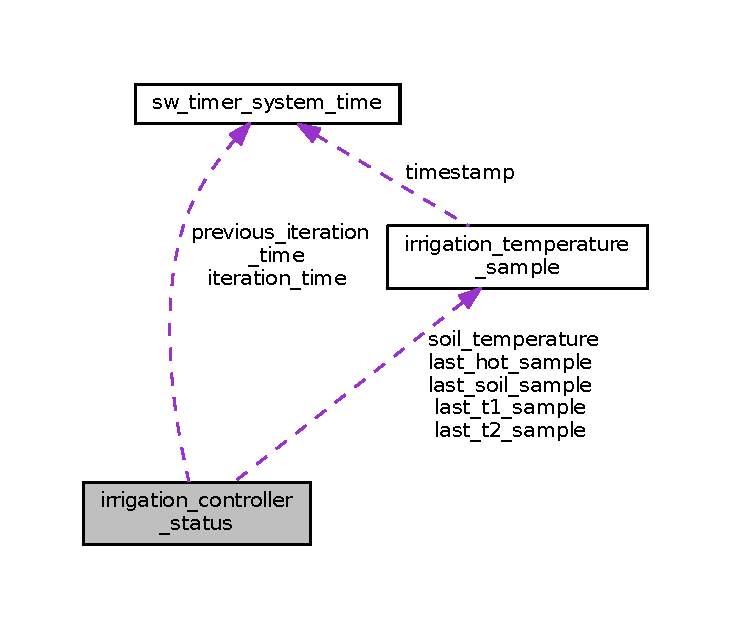
\includegraphics[width=350pt]{structirrigation__controller__status__coll__graph}
\end{center}
\end{figure}
\subsection*{Public Attributes}
\begin{DoxyCompactItemize}
\item 
float \hyperlink{structirrigation__controller__status_a0a4447a8aa2200bacf97bd7e844493c1}{dt}
\begin{DoxyCompactList}\small\item\em Delta time since last state run. \end{DoxyCompactList}\item 
struct \hyperlink{structsw__timer__system__time}{sw\+\_\+timer\+\_\+system\+\_\+time} \hyperlink{structirrigation__controller__status_a1ae5ffb12725754d8309452cf24a2a28}{iteration\+\_\+time}
\begin{DoxyCompactList}\small\item\em Timestamp of when this run started. \end{DoxyCompactList}\item 
struct \hyperlink{structsw__timer__system__time}{sw\+\_\+timer\+\_\+system\+\_\+time} \hyperlink{structirrigation__controller__status_ab5a5ed310a96d8fd4db605bad57bf83a}{previous\+\_\+iteration\+\_\+time}
\begin{DoxyCompactList}\small\item\em Timestamp of previous run, used to calculate \hyperlink{structirrigation__controller__status_a0a4447a8aa2200bacf97bd7e844493c1}{dt}. \end{DoxyCompactList}\item 
\hypertarget{structirrigation__controller__status_a113b7e81a993c20bb5bf90b2faf81bc5}{}enum \hyperlink{irrigation_8h_a9891f6b3b37611d2aebdb8601acdf6c6}{moisture\+\_\+sensor\+\_\+state} {\bfseries sensor\+\_\+state}\label{structirrigation__controller__status_a113b7e81a993c20bb5bf90b2faf81bc5}

\item 
\hypertarget{structirrigation__controller__status_a9f6f7c1cab26fb9200e9ab706098cb98}{}float {\bfseries ackumulative\+\_\+delta\+\_\+temp}\label{structirrigation__controller__status_a9f6f7c1cab26fb9200e9ab706098cb98}

\item 
\hypertarget{structirrigation__controller__status_a6b0753e3ea72f0220cb51e9e14d817ba}{}float {\bfseries ackumulative\+\_\+delta\+\_\+time}\label{structirrigation__controller__status_a6b0753e3ea72f0220cb51e9e14d817ba}

\item 
\hypertarget{structirrigation__controller__status_ae84f5b8517b8fe266305aa248a6f46fc}{}float {\bfseries heating\+\_\+time}\label{structirrigation__controller__status_ae84f5b8517b8fe266305aa248a6f46fc}

\item 
\hypertarget{structirrigation__controller__status_a7b67f38b1433b1909b3afc32fe6b22d9}{}float {\bfseries cooling\+\_\+time}\label{structirrigation__controller__status_a7b67f38b1433b1909b3afc32fe6b22d9}

\item 
struct \hyperlink{structirrigation__temperature__sample}{irrigation\+\_\+temperature\+\_\+sample} \hyperlink{structirrigation__controller__status_a3ef3b031a2c91413170ad02626e8da1c}{soil\+\_\+temperature}
\begin{DoxyCompactList}\small\item\em Last soil temperature measured. \end{DoxyCompactList}\item 
struct \hyperlink{structirrigation__temperature__sample}{irrigation\+\_\+temperature\+\_\+sample} \hyperlink{structirrigation__controller__status_a2d3ef640dc3ec8ce2789fffb092d8f80}{last\+\_\+soil\+\_\+sample}
\begin{DoxyCompactList}\small\item\em Holds the temperature of an initial water content sampling. \end{DoxyCompactList}\item 
struct \hyperlink{structirrigation__temperature__sample}{irrigation\+\_\+temperature\+\_\+sample} \hyperlink{structirrigation__controller__status_ab795e232c4e2d405b11e24312a6163c3}{last\+\_\+hot\+\_\+sample}
\item 
\hypertarget{structirrigation__controller__status_a9b64c69b881c0befd37f25d81141ae24}{}struct \hyperlink{structirrigation__temperature__sample}{irrigation\+\_\+temperature\+\_\+sample} {\bfseries last\+\_\+t1\+\_\+sample}\label{structirrigation__controller__status_a9b64c69b881c0befd37f25d81141ae24}

\item 
\hypertarget{structirrigation__controller__status_af481460c8a71385556ae6a336245fb89}{}struct \hyperlink{structirrigation__temperature__sample}{irrigation\+\_\+temperature\+\_\+sample} {\bfseries last\+\_\+t2\+\_\+sample}\label{structirrigation__controller__status_af481460c8a71385556ae6a336245fb89}

\item 
float \hyperlink{structirrigation__controller__status_a451e58983d5995bf6f1e00f9318d5dd6}{min\+\_\+temperature}
\begin{DoxyCompactList}\small\item\em This is the minimum temperature during \hyperlink{group__state__validate}{Sensor validation state}. \end{DoxyCompactList}\item 
float \hyperlink{structirrigation__controller__status_a1bd8f83a44ee01d3b7cf3851b6716f02}{max\+\_\+temperature}
\begin{DoxyCompactList}\small\item\em This is the minimum temperature during \hyperlink{group__state__validate}{Sensor validation state}. \end{DoxyCompactList}\item 
float \hyperlink{structirrigation__controller__status_a360e7ee7f6ac54635fc66035883d2d9c}{validation\+\_\+timer}
\begin{DoxyCompactList}\small\item\em This is the timer for \hyperlink{group__state__validate}{Sensor validation state}. \end{DoxyCompactList}\item 
float \hyperlink{structirrigation__controller__status_a9d70c74fe395ec2720089b929a32e1e9}{initial\+\_\+timer}
\begin{DoxyCompactList}\small\item\em This is the timer for \hyperlink{group__state__init}{Initial state}. \end{DoxyCompactList}\item 
float \hyperlink{structirrigation__controller__status_aab428bb9e677098d336aefd32b5e6232}{periodic\+\_\+temp\+\_\+report}
\begin{DoxyCompactList}\small\item\em This is a timer for periodic calls to \hyperlink{structirrigation__events_a47b81edd52377b4c4e1ed512b830e237}{irrigation\+\_\+events\+::report\+\_\+current\+\_\+temperature}. \end{DoxyCompactList}\end{DoxyCompactItemize}


\subsection{Detailed Description}


Definition at line 47 of file irrigation.\+h.



\subsection{Member Data Documentation}
\hypertarget{structirrigation__controller__status_a0a4447a8aa2200bacf97bd7e844493c1}{}\index{irrigation\+\_\+controller\+\_\+status@{irrigation\+\_\+controller\+\_\+status}!dt@{dt}}
\index{dt@{dt}!irrigation\+\_\+controller\+\_\+status@{irrigation\+\_\+controller\+\_\+status}}
\subsubsection[{dt}]{\setlength{\rightskip}{0pt plus 5cm}float irrigation\+\_\+controller\+\_\+status\+::dt}\label{structirrigation__controller__status_a0a4447a8aa2200bacf97bd7e844493c1}


Delta time since last state run. 



Definition at line 48 of file irrigation.\+h.



Referenced by state\+\_\+init\+\_\+run(), and state\+\_\+validate\+\_\+run().

\hypertarget{structirrigation__controller__status_a9d70c74fe395ec2720089b929a32e1e9}{}\index{irrigation\+\_\+controller\+\_\+status@{irrigation\+\_\+controller\+\_\+status}!initial\+\_\+timer@{initial\+\_\+timer}}
\index{initial\+\_\+timer@{initial\+\_\+timer}!irrigation\+\_\+controller\+\_\+status@{irrigation\+\_\+controller\+\_\+status}}
\subsubsection[{initial\+\_\+timer}]{\setlength{\rightskip}{0pt plus 5cm}float irrigation\+\_\+controller\+\_\+status\+::initial\+\_\+timer}\label{structirrigation__controller__status_a9d70c74fe395ec2720089b929a32e1e9}


This is the timer for \hyperlink{group__state__init}{Initial state}. 



Definition at line 64 of file irrigation.\+h.



Referenced by state\+\_\+init\+\_\+enter(), and state\+\_\+init\+\_\+run().

\hypertarget{structirrigation__controller__status_a1ae5ffb12725754d8309452cf24a2a28}{}\index{irrigation\+\_\+controller\+\_\+status@{irrigation\+\_\+controller\+\_\+status}!iteration\+\_\+time@{iteration\+\_\+time}}
\index{iteration\+\_\+time@{iteration\+\_\+time}!irrigation\+\_\+controller\+\_\+status@{irrigation\+\_\+controller\+\_\+status}}
\subsubsection[{iteration\+\_\+time}]{\setlength{\rightskip}{0pt plus 5cm}struct {\bf sw\+\_\+timer\+\_\+system\+\_\+time} irrigation\+\_\+controller\+\_\+status\+::iteration\+\_\+time}\label{structirrigation__controller__status_a1ae5ffb12725754d8309452cf24a2a28}


Timestamp of when this run started. 



Definition at line 49 of file irrigation.\+h.



Referenced by state\+\_\+measure\+\_\+enter(), state\+\_\+validate\+\_\+enter(), and state\+\_\+validate\+\_\+run().

\hypertarget{structirrigation__controller__status_ab795e232c4e2d405b11e24312a6163c3}{}\index{irrigation\+\_\+controller\+\_\+status@{irrigation\+\_\+controller\+\_\+status}!last\+\_\+hot\+\_\+sample@{last\+\_\+hot\+\_\+sample}}
\index{last\+\_\+hot\+\_\+sample@{last\+\_\+hot\+\_\+sample}!irrigation\+\_\+controller\+\_\+status@{irrigation\+\_\+controller\+\_\+status}}
\subsubsection[{last\+\_\+hot\+\_\+sample}]{\setlength{\rightskip}{0pt plus 5cm}struct {\bf irrigation\+\_\+temperature\+\_\+sample} irrigation\+\_\+controller\+\_\+status\+::last\+\_\+hot\+\_\+sample}\label{structirrigation__controller__status_ab795e232c4e2d405b11e24312a6163c3}
\begin{DoxyRefDesc}{Todo}
\item[\hyperlink{todo__todo000004}{Todo}]Clean up unused stuff here \end{DoxyRefDesc}


Definition at line 58 of file irrigation.\+h.

\hypertarget{structirrigation__controller__status_a2d3ef640dc3ec8ce2789fffb092d8f80}{}\index{irrigation\+\_\+controller\+\_\+status@{irrigation\+\_\+controller\+\_\+status}!last\+\_\+soil\+\_\+sample@{last\+\_\+soil\+\_\+sample}}
\index{last\+\_\+soil\+\_\+sample@{last\+\_\+soil\+\_\+sample}!irrigation\+\_\+controller\+\_\+status@{irrigation\+\_\+controller\+\_\+status}}
\subsubsection[{last\+\_\+soil\+\_\+sample}]{\setlength{\rightskip}{0pt plus 5cm}struct {\bf irrigation\+\_\+temperature\+\_\+sample} irrigation\+\_\+controller\+\_\+status\+::last\+\_\+soil\+\_\+sample}\label{structirrigation__controller__status_a2d3ef640dc3ec8ce2789fffb092d8f80}


Holds the temperature of an initial water content sampling. 



Definition at line 57 of file irrigation.\+h.



Referenced by state\+\_\+measure\+\_\+enter().

\hypertarget{structirrigation__controller__status_a1bd8f83a44ee01d3b7cf3851b6716f02}{}\index{irrigation\+\_\+controller\+\_\+status@{irrigation\+\_\+controller\+\_\+status}!max\+\_\+temperature@{max\+\_\+temperature}}
\index{max\+\_\+temperature@{max\+\_\+temperature}!irrigation\+\_\+controller\+\_\+status@{irrigation\+\_\+controller\+\_\+status}}
\subsubsection[{max\+\_\+temperature}]{\setlength{\rightskip}{0pt plus 5cm}float irrigation\+\_\+controller\+\_\+status\+::max\+\_\+temperature}\label{structirrigation__controller__status_a1bd8f83a44ee01d3b7cf3851b6716f02}


This is the minimum temperature during \hyperlink{group__state__validate}{Sensor validation state}. 



Definition at line 62 of file irrigation.\+h.



Referenced by state\+\_\+validate\+\_\+enter(), and state\+\_\+validate\+\_\+run().

\hypertarget{structirrigation__controller__status_a451e58983d5995bf6f1e00f9318d5dd6}{}\index{irrigation\+\_\+controller\+\_\+status@{irrigation\+\_\+controller\+\_\+status}!min\+\_\+temperature@{min\+\_\+temperature}}
\index{min\+\_\+temperature@{min\+\_\+temperature}!irrigation\+\_\+controller\+\_\+status@{irrigation\+\_\+controller\+\_\+status}}
\subsubsection[{min\+\_\+temperature}]{\setlength{\rightskip}{0pt plus 5cm}float irrigation\+\_\+controller\+\_\+status\+::min\+\_\+temperature}\label{structirrigation__controller__status_a451e58983d5995bf6f1e00f9318d5dd6}


This is the minimum temperature during \hyperlink{group__state__validate}{Sensor validation state}. 



Definition at line 61 of file irrigation.\+h.



Referenced by state\+\_\+validate\+\_\+enter(), and state\+\_\+validate\+\_\+run().

\hypertarget{structirrigation__controller__status_aab428bb9e677098d336aefd32b5e6232}{}\index{irrigation\+\_\+controller\+\_\+status@{irrigation\+\_\+controller\+\_\+status}!periodic\+\_\+temp\+\_\+report@{periodic\+\_\+temp\+\_\+report}}
\index{periodic\+\_\+temp\+\_\+report@{periodic\+\_\+temp\+\_\+report}!irrigation\+\_\+controller\+\_\+status@{irrigation\+\_\+controller\+\_\+status}}
\subsubsection[{periodic\+\_\+temp\+\_\+report}]{\setlength{\rightskip}{0pt plus 5cm}float irrigation\+\_\+controller\+\_\+status\+::periodic\+\_\+temp\+\_\+report}\label{structirrigation__controller__status_aab428bb9e677098d336aefd32b5e6232}


This is a timer for periodic calls to \hyperlink{structirrigation__events_a47b81edd52377b4c4e1ed512b830e237}{irrigation\+\_\+events\+::report\+\_\+current\+\_\+temperature}. 



Definition at line 65 of file irrigation.\+h.



Referenced by state\+\_\+measure\+\_\+enter().

\hypertarget{structirrigation__controller__status_ab5a5ed310a96d8fd4db605bad57bf83a}{}\index{irrigation\+\_\+controller\+\_\+status@{irrigation\+\_\+controller\+\_\+status}!previous\+\_\+iteration\+\_\+time@{previous\+\_\+iteration\+\_\+time}}
\index{previous\+\_\+iteration\+\_\+time@{previous\+\_\+iteration\+\_\+time}!irrigation\+\_\+controller\+\_\+status@{irrigation\+\_\+controller\+\_\+status}}
\subsubsection[{previous\+\_\+iteration\+\_\+time}]{\setlength{\rightskip}{0pt plus 5cm}struct {\bf sw\+\_\+timer\+\_\+system\+\_\+time} irrigation\+\_\+controller\+\_\+status\+::previous\+\_\+iteration\+\_\+time}\label{structirrigation__controller__status_ab5a5ed310a96d8fd4db605bad57bf83a}


Timestamp of previous run, used to calculate \hyperlink{structirrigation__controller__status_a0a4447a8aa2200bacf97bd7e844493c1}{dt}. 



Definition at line 50 of file irrigation.\+h.

\hypertarget{structirrigation__controller__status_a3ef3b031a2c91413170ad02626e8da1c}{}\index{irrigation\+\_\+controller\+\_\+status@{irrigation\+\_\+controller\+\_\+status}!soil\+\_\+temperature@{soil\+\_\+temperature}}
\index{soil\+\_\+temperature@{soil\+\_\+temperature}!irrigation\+\_\+controller\+\_\+status@{irrigation\+\_\+controller\+\_\+status}}
\subsubsection[{soil\+\_\+temperature}]{\setlength{\rightskip}{0pt plus 5cm}struct {\bf irrigation\+\_\+temperature\+\_\+sample} irrigation\+\_\+controller\+\_\+status\+::soil\+\_\+temperature}\label{structirrigation__controller__status_a3ef3b031a2c91413170ad02626e8da1c}


Last soil temperature measured. 



Definition at line 56 of file irrigation.\+h.



Referenced by state\+\_\+measure\+\_\+enter(), state\+\_\+validate\+\_\+enter(), and state\+\_\+validate\+\_\+run().

\hypertarget{structirrigation__controller__status_a360e7ee7f6ac54635fc66035883d2d9c}{}\index{irrigation\+\_\+controller\+\_\+status@{irrigation\+\_\+controller\+\_\+status}!validation\+\_\+timer@{validation\+\_\+timer}}
\index{validation\+\_\+timer@{validation\+\_\+timer}!irrigation\+\_\+controller\+\_\+status@{irrigation\+\_\+controller\+\_\+status}}
\subsubsection[{validation\+\_\+timer}]{\setlength{\rightskip}{0pt plus 5cm}float irrigation\+\_\+controller\+\_\+status\+::validation\+\_\+timer}\label{structirrigation__controller__status_a360e7ee7f6ac54635fc66035883d2d9c}


This is the timer for \hyperlink{group__state__validate}{Sensor validation state}. 



Definition at line 63 of file irrigation.\+h.



Referenced by state\+\_\+validate\+\_\+enter(), and state\+\_\+validate\+\_\+run().



The documentation for this struct was generated from the following file\+:\begin{DoxyCompactItemize}
\item 
src/\hyperlink{irrigation_8h}{irrigation.\+h}\end{DoxyCompactItemize}

\hypertarget{structirrigation__events}{}\section{irrigation\+\_\+events Struct Reference}
\label{structirrigation__events}\index{irrigation\+\_\+events@{irrigation\+\_\+events}}


The event callback functions for the irrigation controller core.  




{\ttfamily \#include $<$irrigation.\+h$>$}

\subsection*{Public Attributes}
\begin{DoxyCompactItemize}
\item 
void($\ast$ \hyperlink{structirrigation__events_acc5d9d31cce6888cab54d32463470f07}{report\+\_\+validation\+\_\+temperatures} )(struct \hyperlink{structirrigation__controller}{irrigation\+\_\+controller} $\ast$)
\begin{DoxyCompactList}\small\item\em Report the measured temperatures for validation. \end{DoxyCompactList}\item 
void($\ast$ \hyperlink{structirrigation__events_abafd6872889e6e54648653f690e61ec6}{report\+\_\+sensor\+\_\+malfunction} )(struct \hyperlink{structirrigation__controller}{irrigation\+\_\+controller} $\ast$)
\begin{DoxyCompactList}\small\item\em Report that sensordata is invalid. \end{DoxyCompactList}\item 
void($\ast$ \hyperlink{structirrigation__events_a41db6d6a624689abdb7be82425ff0b02}{report\+\_\+sensor\+\_\+fluctuations} )(struct \hyperlink{structirrigation__controller}{irrigation\+\_\+controller} $\ast$)
\begin{DoxyCompactList}\small\item\em Report that sensordata fluctuates. \end{DoxyCompactList}\item 
void($\ast$ \hyperlink{structirrigation__events_a47b81edd52377b4c4e1ed512b830e237}{report\+\_\+current\+\_\+temperature} )(struct \hyperlink{structirrigation__controller}{irrigation\+\_\+controller} $\ast$)
\begin{DoxyCompactList}\small\item\em Reports current temperature. \end{DoxyCompactList}\item 
void($\ast$ \hyperlink{structirrigation__events_add396df12f986fff177801aa022c35f2}{report\+\_\+measurement\+\_\+data} )(struct \hyperlink{structirrigation__controller}{irrigation\+\_\+controller} $\ast$)
\begin{DoxyCompactList}\small\item\em Report water content data. \end{DoxyCompactList}\item 
void($\ast$ \hyperlink{structirrigation__events_aeaa45961cfef7d031a086b2176f4c9a8}{report\+\_\+msg\+\_\+note} )(struct \hyperlink{structirrigation__controller}{irrigation\+\_\+controller} $\ast$, char $\ast$)
\begin{DoxyCompactList}\small\item\em Generic note as a string, used for debugging. \end{DoxyCompactList}\end{DoxyCompactItemize}


\subsection{Detailed Description}
The event callback functions for the irrigation controller core. 

Definition at line 71 of file irrigation.\+h.



\subsection{Member Data Documentation}
\hypertarget{structirrigation__events_a47b81edd52377b4c4e1ed512b830e237}{}\index{irrigation\+\_\+events@{irrigation\+\_\+events}!report\+\_\+current\+\_\+temperature@{report\+\_\+current\+\_\+temperature}}
\index{report\+\_\+current\+\_\+temperature@{report\+\_\+current\+\_\+temperature}!irrigation\+\_\+events@{irrigation\+\_\+events}}
\subsubsection[{report\+\_\+current\+\_\+temperature}]{\setlength{\rightskip}{0pt plus 5cm}void($\ast$ irrigation\+\_\+events\+::report\+\_\+current\+\_\+temperature) (struct {\bf irrigation\+\_\+controller} $\ast$)}\label{structirrigation__events_a47b81edd52377b4c4e1ed512b830e237}


Reports current temperature. 



Definition at line 75 of file irrigation.\+h.

\hypertarget{structirrigation__events_add396df12f986fff177801aa022c35f2}{}\index{irrigation\+\_\+events@{irrigation\+\_\+events}!report\+\_\+measurement\+\_\+data@{report\+\_\+measurement\+\_\+data}}
\index{report\+\_\+measurement\+\_\+data@{report\+\_\+measurement\+\_\+data}!irrigation\+\_\+events@{irrigation\+\_\+events}}
\subsubsection[{report\+\_\+measurement\+\_\+data}]{\setlength{\rightskip}{0pt plus 5cm}void($\ast$ irrigation\+\_\+events\+::report\+\_\+measurement\+\_\+data) (struct {\bf irrigation\+\_\+controller} $\ast$)}\label{structirrigation__events_add396df12f986fff177801aa022c35f2}


Report water content data. 



Definition at line 76 of file irrigation.\+h.

\hypertarget{structirrigation__events_aeaa45961cfef7d031a086b2176f4c9a8}{}\index{irrigation\+\_\+events@{irrigation\+\_\+events}!report\+\_\+msg\+\_\+note@{report\+\_\+msg\+\_\+note}}
\index{report\+\_\+msg\+\_\+note@{report\+\_\+msg\+\_\+note}!irrigation\+\_\+events@{irrigation\+\_\+events}}
\subsubsection[{report\+\_\+msg\+\_\+note}]{\setlength{\rightskip}{0pt plus 5cm}void($\ast$ irrigation\+\_\+events\+::report\+\_\+msg\+\_\+note) (struct {\bf irrigation\+\_\+controller} $\ast$, char $\ast$)}\label{structirrigation__events_aeaa45961cfef7d031a086b2176f4c9a8}


Generic note as a string, used for debugging. 



Definition at line 77 of file irrigation.\+h.



Referenced by state\+\_\+measure\+\_\+enter().

\hypertarget{structirrigation__events_a41db6d6a624689abdb7be82425ff0b02}{}\index{irrigation\+\_\+events@{irrigation\+\_\+events}!report\+\_\+sensor\+\_\+fluctuations@{report\+\_\+sensor\+\_\+fluctuations}}
\index{report\+\_\+sensor\+\_\+fluctuations@{report\+\_\+sensor\+\_\+fluctuations}!irrigation\+\_\+events@{irrigation\+\_\+events}}
\subsubsection[{report\+\_\+sensor\+\_\+fluctuations}]{\setlength{\rightskip}{0pt plus 5cm}void($\ast$ irrigation\+\_\+events\+::report\+\_\+sensor\+\_\+fluctuations) (struct {\bf irrigation\+\_\+controller} $\ast$)}\label{structirrigation__events_a41db6d6a624689abdb7be82425ff0b02}


Report that sensordata fluctuates. 



Definition at line 74 of file irrigation.\+h.



Referenced by state\+\_\+validate\+\_\+run().

\hypertarget{structirrigation__events_abafd6872889e6e54648653f690e61ec6}{}\index{irrigation\+\_\+events@{irrigation\+\_\+events}!report\+\_\+sensor\+\_\+malfunction@{report\+\_\+sensor\+\_\+malfunction}}
\index{report\+\_\+sensor\+\_\+malfunction@{report\+\_\+sensor\+\_\+malfunction}!irrigation\+\_\+events@{irrigation\+\_\+events}}
\subsubsection[{report\+\_\+sensor\+\_\+malfunction}]{\setlength{\rightskip}{0pt plus 5cm}void($\ast$ irrigation\+\_\+events\+::report\+\_\+sensor\+\_\+malfunction) (struct {\bf irrigation\+\_\+controller} $\ast$)}\label{structirrigation__events_abafd6872889e6e54648653f690e61ec6}


Report that sensordata is invalid. 



Definition at line 73 of file irrigation.\+h.



Referenced by state\+\_\+measure\+\_\+enter(), state\+\_\+validate\+\_\+enter(), and state\+\_\+validate\+\_\+run().

\hypertarget{structirrigation__events_acc5d9d31cce6888cab54d32463470f07}{}\index{irrigation\+\_\+events@{irrigation\+\_\+events}!report\+\_\+validation\+\_\+temperatures@{report\+\_\+validation\+\_\+temperatures}}
\index{report\+\_\+validation\+\_\+temperatures@{report\+\_\+validation\+\_\+temperatures}!irrigation\+\_\+events@{irrigation\+\_\+events}}
\subsubsection[{report\+\_\+validation\+\_\+temperatures}]{\setlength{\rightskip}{0pt plus 5cm}void($\ast$ irrigation\+\_\+events\+::report\+\_\+validation\+\_\+temperatures) (struct {\bf irrigation\+\_\+controller} $\ast$)}\label{structirrigation__events_acc5d9d31cce6888cab54d32463470f07}


Report the measured temperatures for validation. 

\begin{DoxySeeAlso}{See also}
\hyperlink{group__state__validate_gac0d41d4685bd461b3a613f6320405b79}{state\+\_\+validate\+\_\+enter} min\+\_\+temperature max\+\_\+temperature 
\end{DoxySeeAlso}


Definition at line 72 of file irrigation.\+h.



Referenced by state\+\_\+validate\+\_\+run().



The documentation for this struct was generated from the following file\+:\begin{DoxyCompactItemize}
\item 
src/\hyperlink{irrigation_8h}{irrigation.\+h}\end{DoxyCompactItemize}

\hypertarget{structirrigation__temperature__sample}{}\section{irrigation\+\_\+temperature\+\_\+sample Struct Reference}
\label{structirrigation__temperature__sample}\index{irrigation\+\_\+temperature\+\_\+sample@{irrigation\+\_\+temperature\+\_\+sample}}


This is a timestamped temperature sample.  




{\ttfamily \#include $<$irrigation.\+h$>$}



Collaboration diagram for irrigation\+\_\+temperature\+\_\+sample\+:\nopagebreak
\begin{figure}[H]
\begin{center}
\leavevmode
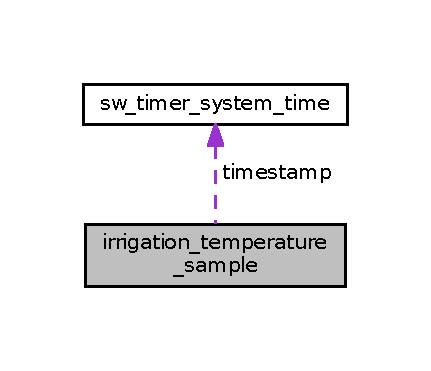
\includegraphics[width=207pt]{structirrigation__temperature__sample__coll__graph}
\end{center}
\end{figure}
\subsection*{Public Attributes}
\begin{DoxyCompactItemize}
\item 
struct \hyperlink{structsw__timer__system__time}{sw\+\_\+timer\+\_\+system\+\_\+time} \hyperlink{structirrigation__temperature__sample_aa10fbbf9f10f89fc9f246f42c26b0ad2}{timestamp}
\begin{DoxyCompactList}\small\item\em Time sample was taken. \end{DoxyCompactList}\item 
float \hyperlink{structirrigation__temperature__sample_ae72c8bc3c16a24366685eecbf9493a2e}{temperature}
\begin{DoxyCompactList}\small\item\em Temperature. \end{DoxyCompactList}\end{DoxyCompactItemize}


\subsection{Detailed Description}
This is a timestamped temperature sample. 

Definition at line 34 of file irrigation.\+h.



\subsection{Member Data Documentation}
\hypertarget{structirrigation__temperature__sample_ae72c8bc3c16a24366685eecbf9493a2e}{}\index{irrigation\+\_\+temperature\+\_\+sample@{irrigation\+\_\+temperature\+\_\+sample}!temperature@{temperature}}
\index{temperature@{temperature}!irrigation\+\_\+temperature\+\_\+sample@{irrigation\+\_\+temperature\+\_\+sample}}
\subsubsection[{temperature}]{\setlength{\rightskip}{0pt plus 5cm}float irrigation\+\_\+temperature\+\_\+sample\+::temperature}\label{structirrigation__temperature__sample_ae72c8bc3c16a24366685eecbf9493a2e}


Temperature. 



Definition at line 36 of file irrigation.\+h.



Referenced by state\+\_\+validate\+\_\+enter(), and state\+\_\+validate\+\_\+run().

\hypertarget{structirrigation__temperature__sample_aa10fbbf9f10f89fc9f246f42c26b0ad2}{}\index{irrigation\+\_\+temperature\+\_\+sample@{irrigation\+\_\+temperature\+\_\+sample}!timestamp@{timestamp}}
\index{timestamp@{timestamp}!irrigation\+\_\+temperature\+\_\+sample@{irrigation\+\_\+temperature\+\_\+sample}}
\subsubsection[{timestamp}]{\setlength{\rightskip}{0pt plus 5cm}struct {\bf sw\+\_\+timer\+\_\+system\+\_\+time} irrigation\+\_\+temperature\+\_\+sample\+::timestamp}\label{structirrigation__temperature__sample_aa10fbbf9f10f89fc9f246f42c26b0ad2}


Time sample was taken. 



Definition at line 35 of file irrigation.\+h.



Referenced by state\+\_\+measure\+\_\+enter(), state\+\_\+validate\+\_\+enter(), and state\+\_\+validate\+\_\+run().



The documentation for this struct was generated from the following file\+:\begin{DoxyCompactItemize}
\item 
src/\hyperlink{irrigation_8h}{irrigation.\+h}\end{DoxyCompactItemize}

\hypertarget{structsw__timer__system__time}{}\section{sw\+\_\+timer\+\_\+system\+\_\+time Struct Reference}
\label{structsw__timer__system__time}\index{sw\+\_\+timer\+\_\+system\+\_\+time@{sw\+\_\+timer\+\_\+system\+\_\+time}}


Timestamp.  




{\ttfamily \#include $<$time.\+h$>$}

\subsection*{Public Attributes}
\begin{DoxyCompactItemize}
\item 
int \hyperlink{structsw__timer__system__time_aa9f10bc219cafbf8c61f94fbb4138591}{epoch}
\begin{DoxyCompactList}\small\item\em Epoch time. \end{DoxyCompactList}\item 
int \hyperlink{structsw__timer__system__time_aafb47623ce45c3d1617e54d2025b679a}{ms}
\begin{DoxyCompactList}\small\item\em Remaining milliseconds. \end{DoxyCompactList}\end{DoxyCompactItemize}


\subsection{Detailed Description}
Timestamp. 

Definition at line 21 of file time.\+h.



\subsection{Member Data Documentation}
\hypertarget{structsw__timer__system__time_aa9f10bc219cafbf8c61f94fbb4138591}{}\index{sw\+\_\+timer\+\_\+system\+\_\+time@{sw\+\_\+timer\+\_\+system\+\_\+time}!epoch@{epoch}}
\index{epoch@{epoch}!sw\+\_\+timer\+\_\+system\+\_\+time@{sw\+\_\+timer\+\_\+system\+\_\+time}}
\subsubsection[{epoch}]{\setlength{\rightskip}{0pt plus 5cm}int sw\+\_\+timer\+\_\+system\+\_\+time\+::epoch}\label{structsw__timer__system__time_aa9f10bc219cafbf8c61f94fbb4138591}


Epoch time. 



Definition at line 22 of file time.\+h.



Referenced by sys\+\_\+tick\+\_\+handler(), and usart\+\_\+blocking\+\_\+tm().

\hypertarget{structsw__timer__system__time_aafb47623ce45c3d1617e54d2025b679a}{}\index{sw\+\_\+timer\+\_\+system\+\_\+time@{sw\+\_\+timer\+\_\+system\+\_\+time}!ms@{ms}}
\index{ms@{ms}!sw\+\_\+timer\+\_\+system\+\_\+time@{sw\+\_\+timer\+\_\+system\+\_\+time}}
\subsubsection[{ms}]{\setlength{\rightskip}{0pt plus 5cm}int sw\+\_\+timer\+\_\+system\+\_\+time\+::ms}\label{structsw__timer__system__time_aafb47623ce45c3d1617e54d2025b679a}


Remaining milliseconds. 



Definition at line 23 of file time.\+h.



Referenced by sys\+\_\+tick\+\_\+handler(), and usart\+\_\+blocking\+\_\+tm().



The documentation for this struct was generated from the following file\+:\begin{DoxyCompactItemize}
\item 
src/\hyperlink{time_8h}{time.\+h}\end{DoxyCompactItemize}

\hypertarget{structsystick}{}\section{systick Struct Reference}
\label{structsystick}\index{systick@{systick}}


Collaboration diagram for systick\+:\nopagebreak
\begin{figure}[H]
\begin{center}
\leavevmode
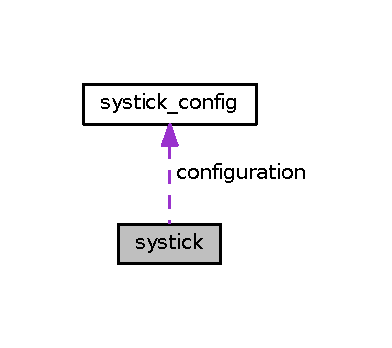
\includegraphics[width=188pt]{structsystick__coll__graph}
\end{center}
\end{figure}
\subsection*{Public Attributes}
\begin{DoxyCompactItemize}
\item 
\hypertarget{structsystick_a6e7d92e68eb2e575624d068b187ace33}{}struct \hyperlink{structsystick__config}{systick\+\_\+config} $\ast$ {\bfseries configuration}\label{structsystick_a6e7d92e68eb2e575624d068b187ace33}

\end{DoxyCompactItemize}


\subsection{Detailed Description}


Definition at line 15 of file systick.\+h.



The documentation for this struct was generated from the following file\+:\begin{DoxyCompactItemize}
\item 
src/\hyperlink{systick_8h}{systick.\+h}\end{DoxyCompactItemize}

\hypertarget{structsystick__config}{}\section{systick\+\_\+config Struct Reference}
\label{structsystick__config}\index{systick\+\_\+config@{systick\+\_\+config}}
\subsection*{Public Attributes}
\begin{DoxyCompactItemize}
\item 
\hypertarget{structsystick__config_a4234a833cb468e5ebe169bef99cb9235}{}uint32\+\_\+t {\bfseries frequency}\label{structsystick__config_a4234a833cb468e5ebe169bef99cb9235}

\item 
\hypertarget{structsystick__config_aa9f9da280ed0e328cdd0d0648a46aaad}{}bool {\bfseries auto\+\_\+start}\label{structsystick__config_aa9f9da280ed0e328cdd0d0648a46aaad}

\end{DoxyCompactItemize}


\subsection{Detailed Description}


Definition at line 10 of file systick.\+h.



The documentation for this struct was generated from the following file\+:\begin{DoxyCompactItemize}
\item 
src/\hyperlink{systick_8h}{systick.\+h}\end{DoxyCompactItemize}

\hypertarget{structtimer}{}\section{timer Struct Reference}
\label{structtimer}\index{timer@{timer}}


Collaboration diagram for timer\+:\nopagebreak
\begin{figure}[H]
\begin{center}
\leavevmode
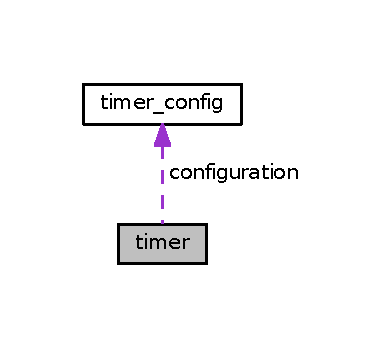
\includegraphics[width=184pt]{structtimer__coll__graph}
\end{center}
\end{figure}
\subsection*{Public Attributes}
\begin{DoxyCompactItemize}
\item 
\hypertarget{structtimer_a2bef740a83dc4af81d0dd6ef45dfbbfd}{}struct \hyperlink{structtimer__config}{timer\+\_\+config} $\ast$ {\bfseries configuration}\label{structtimer_a2bef740a83dc4af81d0dd6ef45dfbbfd}

\item 
\hypertarget{structtimer_a98106a5170cdde683d8bafc2a07ee7cd}{}enum \hyperlink{hw_8h_a3c02952100e7d051b77cdf060ca0ba9b}{hw\+\_\+init\+\_\+state} {\bfseries state}\label{structtimer_a98106a5170cdde683d8bafc2a07ee7cd}

\item 
\hypertarget{structtimer_a879d6cbfcde8edfebb1456b7b4bee2bb}{}uint32\+\_\+t {\bfseries auto\+\_\+reload}\label{structtimer_a879d6cbfcde8edfebb1456b7b4bee2bb}

\end{DoxyCompactItemize}


\subsection{Detailed Description}


Definition at line 34 of file timer.\+h.



The documentation for this struct was generated from the following file\+:\begin{DoxyCompactItemize}
\item 
src/\hyperlink{timer_8h}{timer.\+h}\end{DoxyCompactItemize}

\hypertarget{structtimer__ccr}{}\section{timer\+\_\+ccr Struct Reference}
\label{structtimer__ccr}\index{timer\+\_\+ccr@{timer\+\_\+ccr}}


Collaboration diagram for timer\+\_\+ccr\+:
\nopagebreak
\begin{figure}[H]
\begin{center}
\leavevmode
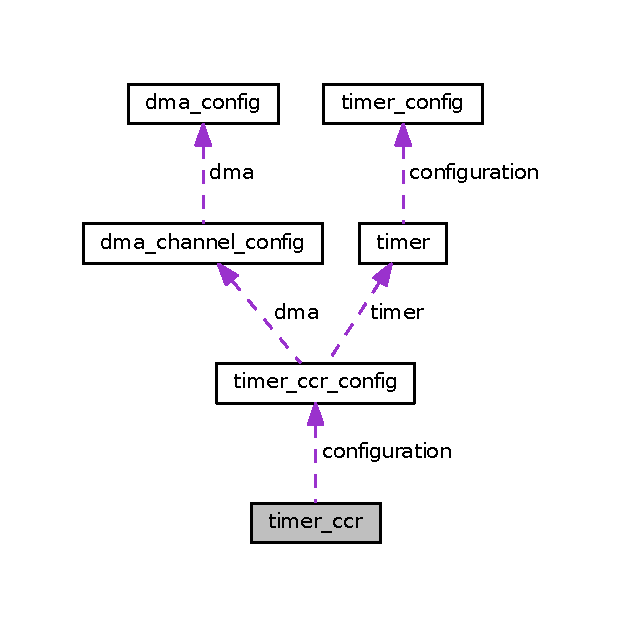
\includegraphics[width=300pt]{structtimer__ccr__coll__graph}
\end{center}
\end{figure}
\subsection*{Public Attributes}
\begin{DoxyCompactItemize}
\item 
\hypertarget{structtimer__ccr_ae53385b34f3535fa8cc732edc5fccc28}{}struct \hyperlink{structtimer__ccr__config}{timer\+\_\+ccr\+\_\+config} $\ast$ {\bfseries configuration}\label{structtimer__ccr_ae53385b34f3535fa8cc732edc5fccc28}

\item 
\hypertarget{structtimer__ccr_addba2954b9a68f87a1e716a65095c6a9}{}enum \hyperlink{hw_8h_a3c02952100e7d051b77cdf060ca0ba9b}{hw\+\_\+init\+\_\+state} {\bfseries state}\label{structtimer__ccr_addba2954b9a68f87a1e716a65095c6a9}

\item 
\hypertarget{structtimer__ccr_a60cdc480531c921c61c6192afff7a0dd}{}uint32\+\_\+t {\bfseries ccr}\label{structtimer__ccr_a60cdc480531c921c61c6192afff7a0dd}

\end{DoxyCompactItemize}


\subsection{Detailed Description}


Definition at line 22 of file timer.\+h.



The documentation for this struct was generated from the following file\+:\begin{DoxyCompactItemize}
\item 
src/\hyperlink{timer_8h}{timer.\+h}\end{DoxyCompactItemize}

\hypertarget{structtimer__ccr__config}{}\section{timer\+\_\+ccr\+\_\+config Struct Reference}
\label{structtimer__ccr__config}\index{timer\+\_\+ccr\+\_\+config@{timer\+\_\+ccr\+\_\+config}}


Collaboration diagram for timer\+\_\+ccr\+\_\+config\+:
\nopagebreak
\begin{figure}[H]
\begin{center}
\leavevmode
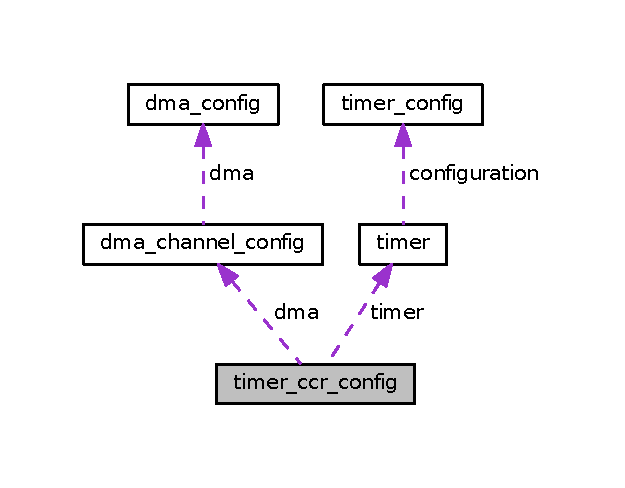
\includegraphics[width=300pt]{structtimer__ccr__config__coll__graph}
\end{center}
\end{figure}
\subsection*{Public Attributes}
\begin{DoxyCompactItemize}
\item 
\hypertarget{structtimer__ccr__config_af228e92c83395be0dff9f27e6ba7711a}{}struct \hyperlink{structtimer}{timer} $\ast$ {\bfseries timer}\label{structtimer__ccr__config_af228e92c83395be0dff9f27e6ba7711a}

\item 
\hypertarget{structtimer__ccr__config_ae497ec8b539565c6fe34b2849989336a}{}enum tim\+\_\+oc\+\_\+id {\bfseries channel}\label{structtimer__ccr__config_ae497ec8b539565c6fe34b2849989336a}

\item 
\hypertarget{structtimer__ccr__config_a1e92f7221c14d90562bd42830fa2427d}{}struct \hyperlink{structdma__channel__config}{dma\+\_\+channel\+\_\+config} $\ast$ {\bfseries dma}\label{structtimer__ccr__config_a1e92f7221c14d90562bd42830fa2427d}

\item 
\hypertarget{structtimer__ccr__config_a3876bca410f69a23790a94f8eb9d73f8}{}volatile uint32\+\_\+t $\ast$ {\bfseries reg}\label{structtimer__ccr__config_a3876bca410f69a23790a94f8eb9d73f8}

\end{DoxyCompactItemize}


\subsection{Detailed Description}


Definition at line 14 of file timer.\+h.



The documentation for this struct was generated from the following file\+:\begin{DoxyCompactItemize}
\item 
src/\hyperlink{timer_8h}{timer.\+h}\end{DoxyCompactItemize}

\hypertarget{structtimer__config}{}\section{timer\+\_\+config Struct Reference}
\label{structtimer__config}\index{timer\+\_\+config@{timer\+\_\+config}}
\subsection*{Public Attributes}
\begin{DoxyCompactItemize}
\item 
\hypertarget{structtimer__config_afed1f1ae48fa09893427efa6b8338b65}{}uint32\+\_\+t {\bfseries timer}\label{structtimer__config_afed1f1ae48fa09893427efa6b8338b65}

\item 
\hypertarget{structtimer__config_a1591c4486ebf07c8ac73e69acbbbbc3a}{}uint32\+\_\+t {\bfseries rcc}\label{structtimer__config_a1591c4486ebf07c8ac73e69acbbbbc3a}

\end{DoxyCompactItemize}


\subsection{Detailed Description}


Definition at line 29 of file timer.\+h.



The documentation for this struct was generated from the following file\+:\begin{DoxyCompactItemize}
\item 
src/\hyperlink{timer_8h}{timer.\+h}\end{DoxyCompactItemize}

\hypertarget{structtm}{}\section{tm Struct Reference}
\label{structtm}\index{tm@{tm}}


Broken down time.  




{\ttfamily \#include $<$time.\+h$>$}

\subsection*{Public Attributes}
\begin{DoxyCompactItemize}
\item 
int \hyperlink{structtm_a4d098a9a5c03a00b2ee61e10851de81e}{tm\+\_\+sec}
\begin{DoxyCompactList}\small\item\em seconds \end{DoxyCompactList}\item 
int \hyperlink{structtm_af414eb7c86cc3099595211eee4d4211b}{tm\+\_\+min}
\begin{DoxyCompactList}\small\item\em minutes \end{DoxyCompactList}\item 
int \hyperlink{structtm_a3e7ca4e37f1abcaf56b8a916c38eb9fe}{tm\+\_\+hour}
\begin{DoxyCompactList}\small\item\em hours \end{DoxyCompactList}\item 
int \hyperlink{structtm_ab8d8904bad43b0c8b96e61941c5b5310}{tm\+\_\+mday}
\begin{DoxyCompactList}\small\item\em day of the month \end{DoxyCompactList}\item 
int \hyperlink{structtm_a112ac36fa2f593777138a417cf031e17}{tm\+\_\+mon}
\begin{DoxyCompactList}\small\item\em month \end{DoxyCompactList}\item 
int \hyperlink{structtm_a33adf78fd6476b2120ce3b9c4a852053}{tm\+\_\+year}
\begin{DoxyCompactList}\small\item\em year \end{DoxyCompactList}\item 
int \hyperlink{structtm_afe81a8c46f1c693c43f259b288859f4f}{tm\+\_\+wday}
\begin{DoxyCompactList}\small\item\em day of the week \end{DoxyCompactList}\item 
int \hyperlink{structtm_a93a0ba77cc23796df84405dcbcc57eb1}{tm\+\_\+yday}
\begin{DoxyCompactList}\small\item\em day in the year \end{DoxyCompactList}\item 
int \hyperlink{structtm_a5645ca0580c8ab2c24f6c2965d9c9f9c}{tm\+\_\+isdst}
\begin{DoxyCompactList}\small\item\em daylight saving time \end{DoxyCompactList}\end{DoxyCompactItemize}


\subsection{Detailed Description}
Broken down time. 

Definition at line 8 of file time.\+h.



\subsection{Member Data Documentation}
\hypertarget{structtm_a3e7ca4e37f1abcaf56b8a916c38eb9fe}{}\index{tm@{tm}!tm\+\_\+hour@{tm\+\_\+hour}}
\index{tm\+\_\+hour@{tm\+\_\+hour}!tm@{tm}}
\subsubsection[{tm\+\_\+hour}]{\setlength{\rightskip}{0pt plus 5cm}int tm\+::tm\+\_\+hour}\label{structtm_a3e7ca4e37f1abcaf56b8a916c38eb9fe}


hours 



Definition at line 11 of file time.\+h.



Referenced by time\+\_\+tm\+\_\+from\+\_\+epoch(), and usart\+\_\+blocking\+\_\+tm().

\hypertarget{structtm_a5645ca0580c8ab2c24f6c2965d9c9f9c}{}\index{tm@{tm}!tm\+\_\+isdst@{tm\+\_\+isdst}}
\index{tm\+\_\+isdst@{tm\+\_\+isdst}!tm@{tm}}
\subsubsection[{tm\+\_\+isdst}]{\setlength{\rightskip}{0pt plus 5cm}int tm\+::tm\+\_\+isdst}\label{structtm_a5645ca0580c8ab2c24f6c2965d9c9f9c}


daylight saving time 



Definition at line 17 of file time.\+h.

\hypertarget{structtm_ab8d8904bad43b0c8b96e61941c5b5310}{}\index{tm@{tm}!tm\+\_\+mday@{tm\+\_\+mday}}
\index{tm\+\_\+mday@{tm\+\_\+mday}!tm@{tm}}
\subsubsection[{tm\+\_\+mday}]{\setlength{\rightskip}{0pt plus 5cm}int tm\+::tm\+\_\+mday}\label{structtm_ab8d8904bad43b0c8b96e61941c5b5310}


day of the month 



Definition at line 12 of file time.\+h.



Referenced by time\+\_\+tm\+\_\+from\+\_\+epoch(), and usart\+\_\+blocking\+\_\+tm().

\hypertarget{structtm_af414eb7c86cc3099595211eee4d4211b}{}\index{tm@{tm}!tm\+\_\+min@{tm\+\_\+min}}
\index{tm\+\_\+min@{tm\+\_\+min}!tm@{tm}}
\subsubsection[{tm\+\_\+min}]{\setlength{\rightskip}{0pt plus 5cm}int tm\+::tm\+\_\+min}\label{structtm_af414eb7c86cc3099595211eee4d4211b}


minutes 



Definition at line 10 of file time.\+h.



Referenced by time\+\_\+tm\+\_\+from\+\_\+epoch(), and usart\+\_\+blocking\+\_\+tm().

\hypertarget{structtm_a112ac36fa2f593777138a417cf031e17}{}\index{tm@{tm}!tm\+\_\+mon@{tm\+\_\+mon}}
\index{tm\+\_\+mon@{tm\+\_\+mon}!tm@{tm}}
\subsubsection[{tm\+\_\+mon}]{\setlength{\rightskip}{0pt plus 5cm}int tm\+::tm\+\_\+mon}\label{structtm_a112ac36fa2f593777138a417cf031e17}


month 



Definition at line 13 of file time.\+h.



Referenced by time\+\_\+tm\+\_\+from\+\_\+epoch(), and usart\+\_\+blocking\+\_\+tm().

\hypertarget{structtm_a4d098a9a5c03a00b2ee61e10851de81e}{}\index{tm@{tm}!tm\+\_\+sec@{tm\+\_\+sec}}
\index{tm\+\_\+sec@{tm\+\_\+sec}!tm@{tm}}
\subsubsection[{tm\+\_\+sec}]{\setlength{\rightskip}{0pt plus 5cm}int tm\+::tm\+\_\+sec}\label{structtm_a4d098a9a5c03a00b2ee61e10851de81e}


seconds 



Definition at line 9 of file time.\+h.



Referenced by time\+\_\+tm\+\_\+from\+\_\+epoch(), and usart\+\_\+blocking\+\_\+tm().

\hypertarget{structtm_afe81a8c46f1c693c43f259b288859f4f}{}\index{tm@{tm}!tm\+\_\+wday@{tm\+\_\+wday}}
\index{tm\+\_\+wday@{tm\+\_\+wday}!tm@{tm}}
\subsubsection[{tm\+\_\+wday}]{\setlength{\rightskip}{0pt plus 5cm}int tm\+::tm\+\_\+wday}\label{structtm_afe81a8c46f1c693c43f259b288859f4f}


day of the week 



Definition at line 15 of file time.\+h.



Referenced by time\+\_\+tm\+\_\+from\+\_\+epoch().

\hypertarget{structtm_a93a0ba77cc23796df84405dcbcc57eb1}{}\index{tm@{tm}!tm\+\_\+yday@{tm\+\_\+yday}}
\index{tm\+\_\+yday@{tm\+\_\+yday}!tm@{tm}}
\subsubsection[{tm\+\_\+yday}]{\setlength{\rightskip}{0pt plus 5cm}int tm\+::tm\+\_\+yday}\label{structtm_a93a0ba77cc23796df84405dcbcc57eb1}


day in the year 



Definition at line 16 of file time.\+h.



Referenced by time\+\_\+tm\+\_\+from\+\_\+epoch().

\hypertarget{structtm_a33adf78fd6476b2120ce3b9c4a852053}{}\index{tm@{tm}!tm\+\_\+year@{tm\+\_\+year}}
\index{tm\+\_\+year@{tm\+\_\+year}!tm@{tm}}
\subsubsection[{tm\+\_\+year}]{\setlength{\rightskip}{0pt plus 5cm}int tm\+::tm\+\_\+year}\label{structtm_a33adf78fd6476b2120ce3b9c4a852053}


year 



Definition at line 14 of file time.\+h.



Referenced by time\+\_\+tm\+\_\+from\+\_\+epoch(), and usart\+\_\+blocking\+\_\+tm().



The documentation for this struct was generated from the following file\+:\begin{DoxyCompactItemize}
\item 
src/\hyperlink{time_8h}{time.\+h}\end{DoxyCompactItemize}

\hypertarget{structusart}{}\section{usart Struct Reference}
\label{structusart}\index{usart@{usart}}


Usart.  




{\ttfamily \#include $<$uart.\+h$>$}



Collaboration diagram for usart\+:\nopagebreak
\begin{figure}[H]
\begin{center}
\leavevmode
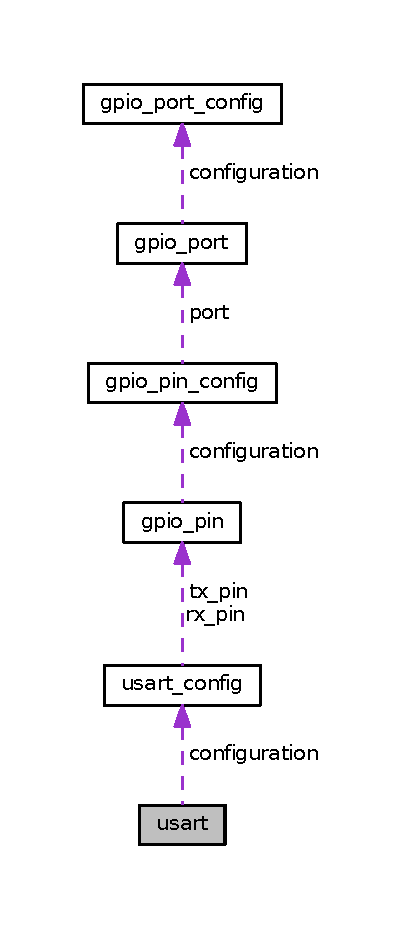
\includegraphics[width=194pt]{structusart__coll__graph}
\end{center}
\end{figure}
\subsection*{Public Attributes}
\begin{DoxyCompactItemize}
\item 
\hypertarget{structusart_a42f49f07a75c1ec44a8a1e04e08a760c}{}struct \hyperlink{structusart__config}{usart\+\_\+config} $\ast$ {\bfseries configuration}\label{structusart_a42f49f07a75c1ec44a8a1e04e08a760c}

\end{DoxyCompactItemize}


\subsection{Detailed Description}
Usart. 

Definition at line 29 of file uart.\+h.



The documentation for this struct was generated from the following file\+:\begin{DoxyCompactItemize}
\item 
src/\hyperlink{uart_8h}{uart.\+h}\end{DoxyCompactItemize}

\hypertarget{structusart__config}{}\section{usart\+\_\+config Struct Reference}
\label{structusart__config}\index{usart\+\_\+config@{usart\+\_\+config}}


Usart configuration.  




{\ttfamily \#include $<$uart.\+h$>$}



Collaboration diagram for usart\+\_\+config\+:\nopagebreak
\begin{figure}[H]
\begin{center}
\leavevmode
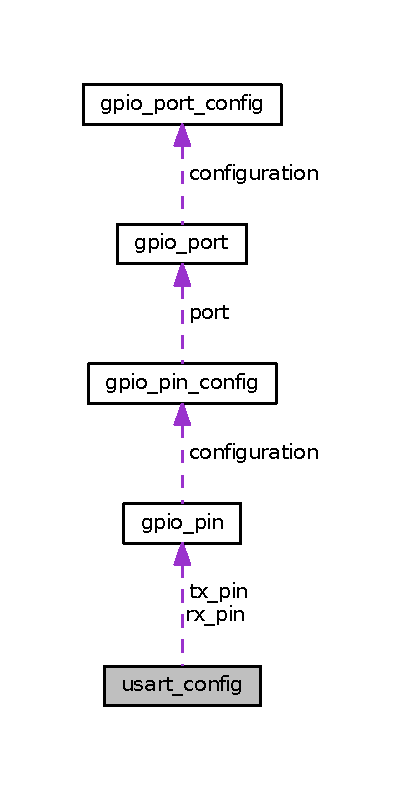
\includegraphics[width=194pt]{structusart__config__coll__graph}
\end{center}
\end{figure}
\subsection*{Public Attributes}
\begin{DoxyCompactItemize}
\item 
\hypertarget{structusart__config_afb0c0a9281bba234d1b7282fd5661826}{}struct \hyperlink{structgpio__pin}{gpio\+\_\+pin} $\ast$ {\bfseries rx\+\_\+pin}\label{structusart__config_afb0c0a9281bba234d1b7282fd5661826}

\item 
\hypertarget{structusart__config_acda049cae41a8261b02b52ef76830941}{}struct \hyperlink{structgpio__pin}{gpio\+\_\+pin} $\ast$ {\bfseries tx\+\_\+pin}\label{structusart__config_acda049cae41a8261b02b52ef76830941}

\item 
\hypertarget{structusart__config_a7057d1e4e59d4cb6f002cace870fa34b}{}uint32\+\_\+t {\bfseries usart}\label{structusart__config_a7057d1e4e59d4cb6f002cace870fa34b}

\item 
\hypertarget{structusart__config_a5362ef6b4daf5a9e2722c9c4e167e9ed}{}uint32\+\_\+t {\bfseries rcc}\label{structusart__config_a5362ef6b4daf5a9e2722c9c4e167e9ed}

\item 
\hypertarget{structusart__config_acacbd7ecb3d46f576ff1361ae40019fd}{}uint32\+\_\+t {\bfseries baudrate}\label{structusart__config_acacbd7ecb3d46f576ff1361ae40019fd}

\item 
\hypertarget{structusart__config_a688b390f173cc710c95227d84a8f0771}{}uint32\+\_\+t {\bfseries databits}\label{structusart__config_a688b390f173cc710c95227d84a8f0771}

\item 
\hypertarget{structusart__config_a69189444320b793047313d2e80c9df6b}{}uint32\+\_\+t {\bfseries parity}\label{structusart__config_a69189444320b793047313d2e80c9df6b}

\item 
\hypertarget{structusart__config_a5d944fbbe5a88c9a2f2d60df6a092f69}{}uint32\+\_\+t {\bfseries stopbits}\label{structusart__config_a5d944fbbe5a88c9a2f2d60df6a092f69}

\item 
\hypertarget{structusart__config_afaf14d61e3be8a4d3208a1acb68967d4}{}uint32\+\_\+t {\bfseries mode}\label{structusart__config_afaf14d61e3be8a4d3208a1acb68967d4}

\item 
\hypertarget{structusart__config_aef2d53d38b3b8b974a5e3355061f9ec8}{}uint32\+\_\+t {\bfseries flowcontrol}\label{structusart__config_aef2d53d38b3b8b974a5e3355061f9ec8}

\end{DoxyCompactItemize}


\subsection{Detailed Description}
Usart configuration. 

Definition at line 14 of file uart.\+h.



The documentation for this struct was generated from the following file\+:\begin{DoxyCompactItemize}
\item 
src/\hyperlink{uart_8h}{uart.\+h}\end{DoxyCompactItemize}

\hypertarget{structws2812}{}\section{ws2812 Struct Reference}
\label{structws2812}\index{ws2812@{ws2812}}


W\+S2812 Instance.  




{\ttfamily \#include $<$ws2812.\+h$>$}



Collaboration diagram for ws2812\+:\nopagebreak
\begin{figure}[H]
\begin{center}
\leavevmode
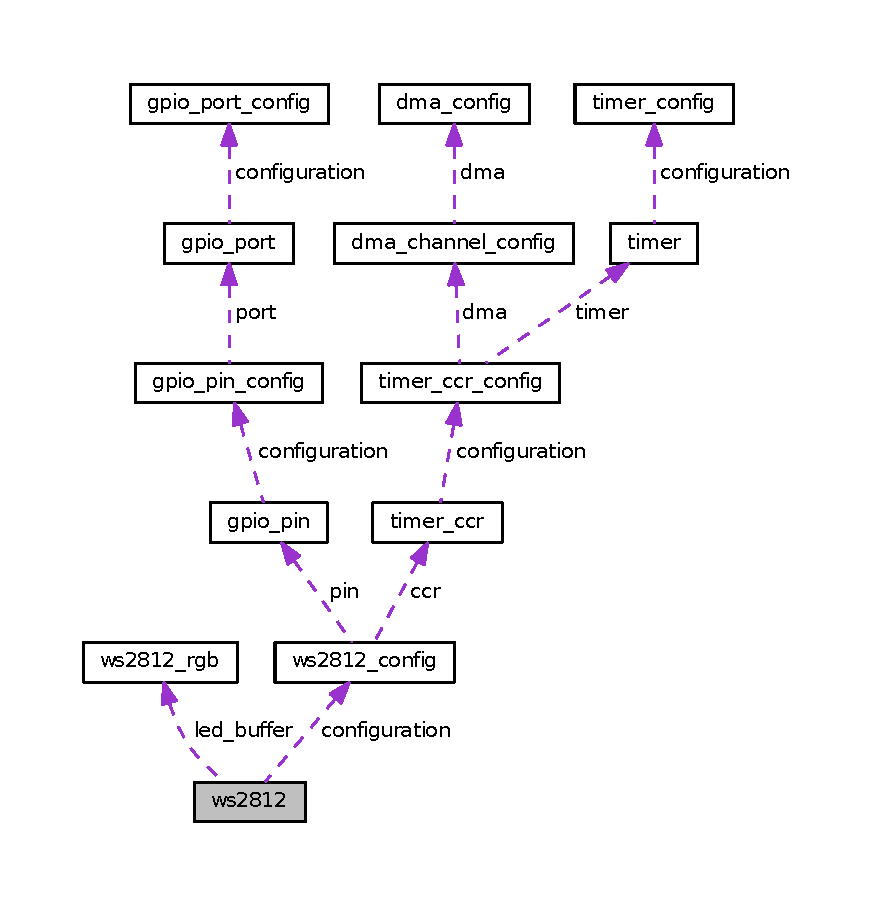
\includegraphics[width=350pt]{structws2812__coll__graph}
\end{center}
\end{figure}
\subsection*{Public Attributes}
\begin{DoxyCompactItemize}
\item 
struct \hyperlink{structws2812__config}{ws2812\+\_\+config} $\ast$ \hyperlink{structws2812_a4b69cc515557cd305ebfd3372fc09f81}{configuration}
\begin{DoxyCompactList}\small\item\em Pointer to configuration. \end{DoxyCompactList}\item 
struct \hyperlink{structws2812__rgb}{ws2812\+\_\+rgb} $\ast$ \hyperlink{structws2812_a9d672a2d9ea381c7fcd940ba4ebdebe2}{led\+\_\+buffer}
\begin{DoxyCompactList}\small\item\em Pointer to L\+E\+D array. \end{DoxyCompactList}\item 
volatile uint8\+\_\+t $\ast$ \hyperlink{structws2812_a864f88183104cfbdd144cb301870e655}{pwm\+\_\+buffer}
\begin{DoxyCompactList}\small\item\em Pointer to buffer for P\+W\+M data. \end{DoxyCompactList}\item 
enum \hyperlink{hw_8h_a3c02952100e7d051b77cdf060ca0ba9b}{hw\+\_\+init\+\_\+state} \hyperlink{structws2812_a396b295c928e75adc5688c49c832e631}{state}
\begin{DoxyCompactList}\small\item\em Device state. \end{DoxyCompactList}\item 
int \hyperlink{structws2812_aaed6db83ce4a0e8e58b73650f2b4638e}{led\+\_\+count}
\begin{DoxyCompactList}\small\item\em Number of L\+E\+Ds connected to the bus. \end{DoxyCompactList}\end{DoxyCompactItemize}


\subsection{Detailed Description}
W\+S2812 Instance. 

Definition at line 21 of file ws2812.\+h.



\subsection{Member Data Documentation}
\hypertarget{structws2812_a4b69cc515557cd305ebfd3372fc09f81}{}\index{ws2812@{ws2812}!configuration@{configuration}}
\index{configuration@{configuration}!ws2812@{ws2812}}
\subsubsection[{configuration}]{\setlength{\rightskip}{0pt plus 5cm}struct {\bf ws2812\+\_\+config}$\ast$ ws2812\+::configuration}\label{structws2812_a4b69cc515557cd305ebfd3372fc09f81}


Pointer to configuration. 



Definition at line 22 of file ws2812.\+h.



Referenced by ws2812\+\_\+configure\+\_\+gpio(), ws2812\+\_\+configure\+\_\+timer(), ws2812\+\_\+init(), ws2812\+\_\+process\+\_\+buffer(), ws2812\+\_\+set\+\_\+defaults(), ws2812\+\_\+update(), and ws2812\+\_\+update\+\_\+blocking().

\hypertarget{structws2812_a9d672a2d9ea381c7fcd940ba4ebdebe2}{}\index{ws2812@{ws2812}!led\+\_\+buffer@{led\+\_\+buffer}}
\index{led\+\_\+buffer@{led\+\_\+buffer}!ws2812@{ws2812}}
\subsubsection[{led\+\_\+buffer}]{\setlength{\rightskip}{0pt plus 5cm}struct {\bf ws2812\+\_\+rgb}$\ast$ ws2812\+::led\+\_\+buffer}\label{structws2812_a9d672a2d9ea381c7fcd940ba4ebdebe2}


Pointer to L\+E\+D array. 

\begin{DoxyNote}{Note}
This should contain as many elements as there are L\+E\+Ds 
\end{DoxyNote}


Definition at line 23 of file ws2812.\+h.



Referenced by ws2812\+\_\+process\+\_\+buffer(), and ws2812\+\_\+set\+\_\+led().

\hypertarget{structws2812_aaed6db83ce4a0e8e58b73650f2b4638e}{}\index{ws2812@{ws2812}!led\+\_\+count@{led\+\_\+count}}
\index{led\+\_\+count@{led\+\_\+count}!ws2812@{ws2812}}
\subsubsection[{led\+\_\+count}]{\setlength{\rightskip}{0pt plus 5cm}int ws2812\+::led\+\_\+count}\label{structws2812_aaed6db83ce4a0e8e58b73650f2b4638e}


Number of L\+E\+Ds connected to the bus. 



Definition at line 26 of file ws2812.\+h.



Referenced by ws2812\+\_\+process\+\_\+buffer(), ws2812\+\_\+update(), and ws2812\+\_\+update\+\_\+blocking().

\hypertarget{structws2812_a864f88183104cfbdd144cb301870e655}{}\index{ws2812@{ws2812}!pwm\+\_\+buffer@{pwm\+\_\+buffer}}
\index{pwm\+\_\+buffer@{pwm\+\_\+buffer}!ws2812@{ws2812}}
\subsubsection[{pwm\+\_\+buffer}]{\setlength{\rightskip}{0pt plus 5cm}volatile uint8\+\_\+t$\ast$ ws2812\+::pwm\+\_\+buffer}\label{structws2812_a864f88183104cfbdd144cb301870e655}


Pointer to buffer for P\+W\+M data. 

\begin{DoxyNote}{Note}
This should contain 24 $\ast$ N + 1 elements where N is number of L\+E\+Ds 
\end{DoxyNote}


Definition at line 24 of file ws2812.\+h.



Referenced by ws2812\+\_\+process\+\_\+buffer(), ws2812\+\_\+update(), and ws2812\+\_\+update\+\_\+blocking().

\hypertarget{structws2812_a396b295c928e75adc5688c49c832e631}{}\index{ws2812@{ws2812}!state@{state}}
\index{state@{state}!ws2812@{ws2812}}
\subsubsection[{state}]{\setlength{\rightskip}{0pt plus 5cm}enum {\bf hw\+\_\+init\+\_\+state} ws2812\+::state}\label{structws2812_a396b295c928e75adc5688c49c832e631}


Device state. 



Definition at line 25 of file ws2812.\+h.



The documentation for this struct was generated from the following file\+:\begin{DoxyCompactItemize}
\item 
src/\hyperlink{ws2812_8h}{ws2812.\+h}\end{DoxyCompactItemize}

\hypertarget{structws2812__config}{}\section{ws2812\+\_\+config Struct Reference}
\label{structws2812__config}\index{ws2812\+\_\+config@{ws2812\+\_\+config}}


Configuration for W\+S2812.  




{\ttfamily \#include $<$ws2812.\+h$>$}



Collaboration diagram for ws2812\+\_\+config\+:\nopagebreak
\begin{figure}[H]
\begin{center}
\leavevmode
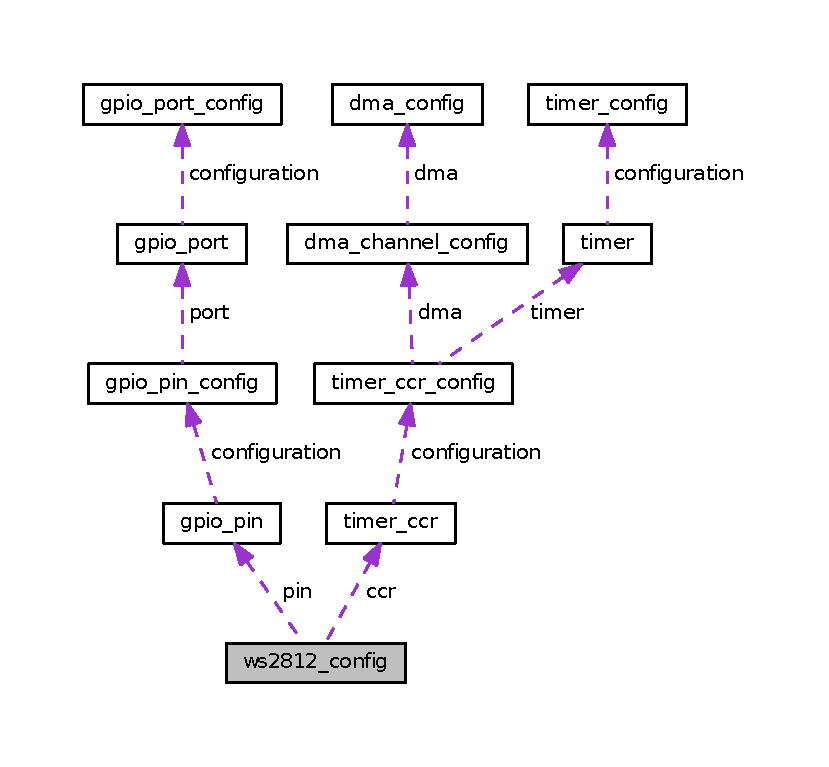
\includegraphics[width=350pt]{structws2812__config__coll__graph}
\end{center}
\end{figure}
\subsection*{Public Attributes}
\begin{DoxyCompactItemize}
\item 
struct \hyperlink{structtimer__ccr}{timer\+\_\+ccr} $\ast$ \hyperlink{structws2812__config_a0c4b50ce11c055c0457af653c4951ee9}{ccr}
\begin{DoxyCompactList}\small\item\em What C\+C\+R to use. \end{DoxyCompactList}\item 
struct \hyperlink{structgpio__pin}{gpio\+\_\+pin} $\ast$ \hyperlink{structws2812__config_a665ce3190145f97af1d234f9de5defc1}{pin}
\begin{DoxyCompactList}\small\item\em What G\+P\+I\+O pin to use. \end{DoxyCompactList}\item 
uint32\+\_\+t \hyperlink{structws2812__config_a15634a419d7f20275ec1e6ba1215920b}{frequency}
\begin{DoxyCompactList}\small\item\em Frequency of data, defaults to 800k\+Hz. \end{DoxyCompactList}\item 
uint32\+\_\+t \hyperlink{structws2812__config_a22370b6dc4cdf5c6e25c4c155a275046}{bit0}
\begin{DoxyCompactList}\small\item\em Length of bit 0 for P\+W\+M. \end{DoxyCompactList}\item 
uint32\+\_\+t \hyperlink{structws2812__config_a410b277b06bbb4ff2f8fd8c6fb5bc994}{bit1}
\begin{DoxyCompactList}\small\item\em Length of bit 1 for P\+W\+M. \end{DoxyCompactList}\end{DoxyCompactItemize}


\subsection{Detailed Description}
Configuration for W\+S2812. 

Definition at line 12 of file ws2812.\+h.



\subsection{Member Data Documentation}
\hypertarget{structws2812__config_a22370b6dc4cdf5c6e25c4c155a275046}{}\index{ws2812\+\_\+config@{ws2812\+\_\+config}!bit0@{bit0}}
\index{bit0@{bit0}!ws2812\+\_\+config@{ws2812\+\_\+config}}
\subsubsection[{bit0}]{\setlength{\rightskip}{0pt plus 5cm}uint32\+\_\+t ws2812\+\_\+config\+::bit0}\label{structws2812__config_a22370b6dc4cdf5c6e25c4c155a275046}


Length of bit 0 for P\+W\+M. 



Definition at line 16 of file ws2812.\+h.



Referenced by ws2812\+\_\+process\+\_\+buffer(), and ws2812\+\_\+set\+\_\+defaults().

\hypertarget{structws2812__config_a410b277b06bbb4ff2f8fd8c6fb5bc994}{}\index{ws2812\+\_\+config@{ws2812\+\_\+config}!bit1@{bit1}}
\index{bit1@{bit1}!ws2812\+\_\+config@{ws2812\+\_\+config}}
\subsubsection[{bit1}]{\setlength{\rightskip}{0pt plus 5cm}uint32\+\_\+t ws2812\+\_\+config\+::bit1}\label{structws2812__config_a410b277b06bbb4ff2f8fd8c6fb5bc994}


Length of bit 1 for P\+W\+M. 



Definition at line 17 of file ws2812.\+h.



Referenced by ws2812\+\_\+process\+\_\+buffer(), and ws2812\+\_\+set\+\_\+defaults().

\hypertarget{structws2812__config_a0c4b50ce11c055c0457af653c4951ee9}{}\index{ws2812\+\_\+config@{ws2812\+\_\+config}!ccr@{ccr}}
\index{ccr@{ccr}!ws2812\+\_\+config@{ws2812\+\_\+config}}
\subsubsection[{ccr}]{\setlength{\rightskip}{0pt plus 5cm}struct {\bf timer\+\_\+ccr}$\ast$ ws2812\+\_\+config\+::ccr}\label{structws2812__config_a0c4b50ce11c055c0457af653c4951ee9}


What C\+C\+R to use. 



Definition at line 13 of file ws2812.\+h.



Referenced by ws2812\+\_\+configure\+\_\+timer(), ws2812\+\_\+init(), ws2812\+\_\+update(), and ws2812\+\_\+update\+\_\+blocking().

\hypertarget{structws2812__config_a15634a419d7f20275ec1e6ba1215920b}{}\index{ws2812\+\_\+config@{ws2812\+\_\+config}!frequency@{frequency}}
\index{frequency@{frequency}!ws2812\+\_\+config@{ws2812\+\_\+config}}
\subsubsection[{frequency}]{\setlength{\rightskip}{0pt plus 5cm}uint32\+\_\+t ws2812\+\_\+config\+::frequency}\label{structws2812__config_a15634a419d7f20275ec1e6ba1215920b}


Frequency of data, defaults to 800k\+Hz. 



Definition at line 15 of file ws2812.\+h.



Referenced by ws2812\+\_\+configure\+\_\+timer(), and ws2812\+\_\+set\+\_\+defaults().

\hypertarget{structws2812__config_a665ce3190145f97af1d234f9de5defc1}{}\index{ws2812\+\_\+config@{ws2812\+\_\+config}!pin@{pin}}
\index{pin@{pin}!ws2812\+\_\+config@{ws2812\+\_\+config}}
\subsubsection[{pin}]{\setlength{\rightskip}{0pt plus 5cm}struct {\bf gpio\+\_\+pin}$\ast$ ws2812\+\_\+config\+::pin}\label{structws2812__config_a665ce3190145f97af1d234f9de5defc1}


What G\+P\+I\+O pin to use. 



Definition at line 14 of file ws2812.\+h.



Referenced by ws2812\+\_\+configure\+\_\+gpio(), and ws2812\+\_\+init().



The documentation for this struct was generated from the following file\+:\begin{DoxyCompactItemize}
\item 
src/\hyperlink{ws2812_8h}{ws2812.\+h}\end{DoxyCompactItemize}

\hypertarget{structws2812__rgb}{}\section{ws2812\+\_\+rgb Struct Reference}
\label{structws2812__rgb}\index{ws2812\+\_\+rgb@{ws2812\+\_\+rgb}}


24 bit color  




{\ttfamily \#include $<$ws2812.\+h$>$}

\subsection*{Public Attributes}
\begin{DoxyCompactItemize}
\item 
uint8\+\_\+t \hyperlink{structws2812__rgb_accf7188c624788256477c2e4ee54515b}{r}
\begin{DoxyCompactList}\small\item\em Red 0-\/255. \end{DoxyCompactList}\item 
uint8\+\_\+t \hyperlink{structws2812__rgb_aaf5b0f4db796641e1cd16bd4f70fc7ac}{g}
\begin{DoxyCompactList}\small\item\em Green 0-\/255. \end{DoxyCompactList}\item 
uint8\+\_\+t \hyperlink{structws2812__rgb_ae6d6d19362a79c36178203b3123d2e7e}{b}
\begin{DoxyCompactList}\small\item\em Blue 0-\/255. \end{DoxyCompactList}\end{DoxyCompactItemize}


\subsection{Detailed Description}
24 bit color 

Definition at line 30 of file ws2812.\+h.



\subsection{Member Data Documentation}
\hypertarget{structws2812__rgb_ae6d6d19362a79c36178203b3123d2e7e}{}\index{ws2812\+\_\+rgb@{ws2812\+\_\+rgb}!b@{b}}
\index{b@{b}!ws2812\+\_\+rgb@{ws2812\+\_\+rgb}}
\subsubsection[{b}]{\setlength{\rightskip}{0pt plus 5cm}uint8\+\_\+t ws2812\+\_\+rgb\+::b}\label{structws2812__rgb_ae6d6d19362a79c36178203b3123d2e7e}


Blue 0-\/255. 



Definition at line 33 of file ws2812.\+h.



Referenced by ws2812\+\_\+process\+\_\+buffer().

\hypertarget{structws2812__rgb_aaf5b0f4db796641e1cd16bd4f70fc7ac}{}\index{ws2812\+\_\+rgb@{ws2812\+\_\+rgb}!g@{g}}
\index{g@{g}!ws2812\+\_\+rgb@{ws2812\+\_\+rgb}}
\subsubsection[{g}]{\setlength{\rightskip}{0pt plus 5cm}uint8\+\_\+t ws2812\+\_\+rgb\+::g}\label{structws2812__rgb_aaf5b0f4db796641e1cd16bd4f70fc7ac}


Green 0-\/255. 



Definition at line 32 of file ws2812.\+h.



Referenced by ws2812\+\_\+process\+\_\+buffer(), and ws2812\+\_\+set\+\_\+led().

\hypertarget{structws2812__rgb_accf7188c624788256477c2e4ee54515b}{}\index{ws2812\+\_\+rgb@{ws2812\+\_\+rgb}!r@{r}}
\index{r@{r}!ws2812\+\_\+rgb@{ws2812\+\_\+rgb}}
\subsubsection[{r}]{\setlength{\rightskip}{0pt plus 5cm}uint8\+\_\+t ws2812\+\_\+rgb\+::r}\label{structws2812__rgb_accf7188c624788256477c2e4ee54515b}


Red 0-\/255. 



Definition at line 31 of file ws2812.\+h.



Referenced by ws2812\+\_\+process\+\_\+buffer(), and ws2812\+\_\+set\+\_\+led().



The documentation for this struct was generated from the following file\+:\begin{DoxyCompactItemize}
\item 
src/\hyperlink{ws2812_8h}{ws2812.\+h}\end{DoxyCompactItemize}

\chapter{File Documentation}
\hypertarget{adc_8c}{}\section{src/adc.c File Reference}
\label{adc_8c}\index{src/adc.\+c@{src/adc.\+c}}


A\+D\+C H\+A\+L implementation.  


{\ttfamily \#include \char`\"{}adc.\+h\char`\"{}}\\*
{\ttfamily \#include \char`\"{}timer.\+h\char`\"{}}\\*
{\ttfamily \#include $<$libopencm3/cm3/nvic.\+h$>$}\\*
Include dependency graph for adc.\+c\+:
\nopagebreak
\begin{figure}[H]
\begin{center}
\leavevmode
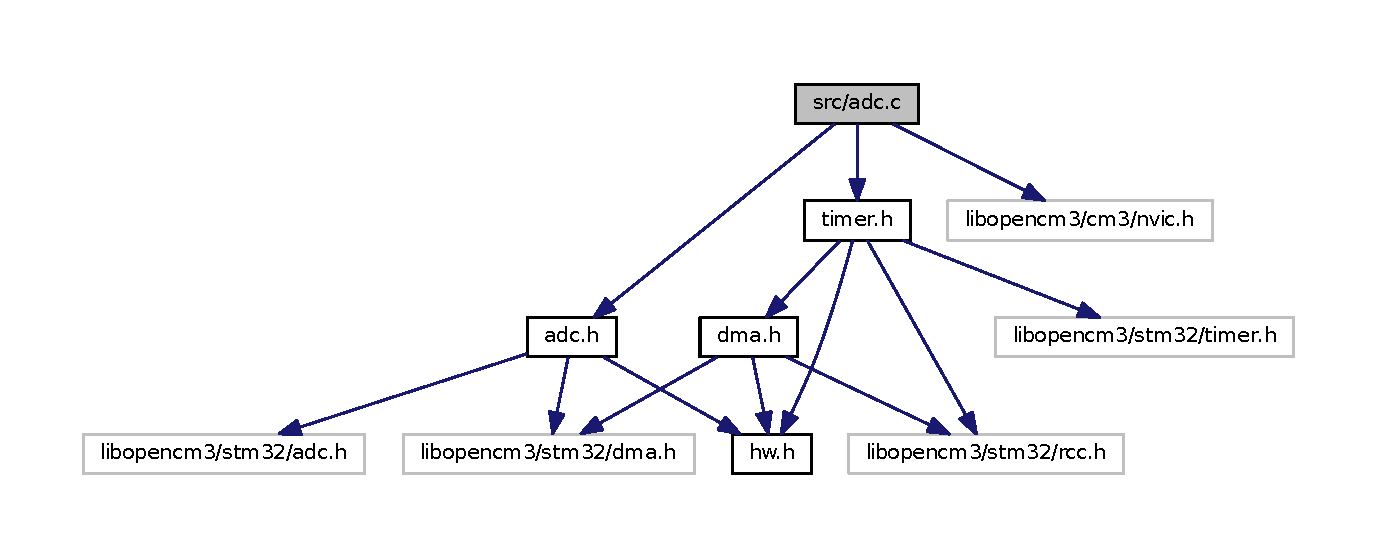
\includegraphics[width=350pt]{adc_8c__incl}
\end{center}
\end{figure}
\subsection*{Functions}
\begin{DoxyCompactItemize}
\item 
\hypertarget{adc_8c_a1c6689c4974ca47f5e316799961c1bab}{}void {\bfseries adc\+\_\+init} (struct \hyperlink{structadc}{adc} $\ast$\hyperlink{structadc}{adc}, enum \hyperlink{hw_8h_a3c02952100e7d051b77cdf060ca0ba9b}{hw\+\_\+init\+\_\+state} state)\label{adc_8c_a1c6689c4974ca47f5e316799961c1bab}

\item 
\hypertarget{adc_8c_ada0028bb1d8d2d158dbcdd17601f54bb}{}void {\bfseries adc\+\_\+begin\+\_\+sampling} (struct \hyperlink{structadc}{adc} $\ast$\hyperlink{structadc}{adc})\label{adc_8c_ada0028bb1d8d2d158dbcdd17601f54bb}

\end{DoxyCompactItemize}
\subsection*{Variables}
\begin{DoxyCompactItemize}
\item 
\hypertarget{adc_8c_afb3b2b082f473dc9b02f36c3d5fd9296}{}static struct \hyperlink{structadc}{adc} $\ast$ {\bfseries adc1} = 0\label{adc_8c_afb3b2b082f473dc9b02f36c3d5fd9296}

\end{DoxyCompactItemize}


\subsection{Detailed Description}
A\+D\+C H\+A\+L implementation. 


\hypertarget{adc_8h}{}\section{src/adc.h File Reference}
\label{adc_8h}\index{src/adc.\+h@{src/adc.\+h}}


A\+D\+C H\+A\+L include.  


{\ttfamily \#include \char`\"{}hw.\+h\char`\"{}}\\*
{\ttfamily \#include $<$libopencm3/stm32/adc.\+h$>$}\\*
{\ttfamily \#include $<$libopencm3/stm32/dma.\+h$>$}\\*
Include dependency graph for adc.\+h\+:\nopagebreak
\begin{figure}[H]
\begin{center}
\leavevmode
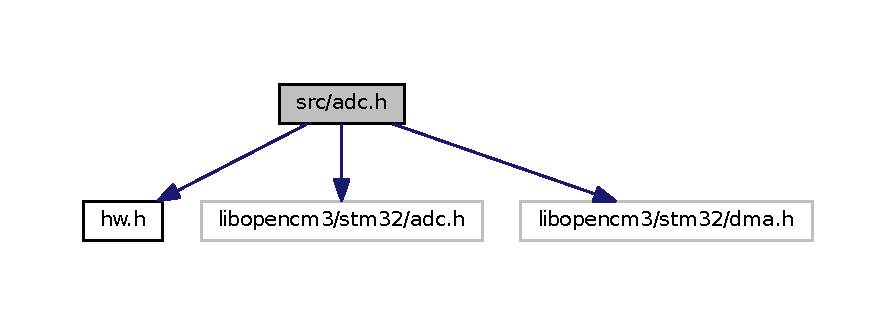
\includegraphics[width=350pt]{adc_8h__incl}
\end{center}
\end{figure}
This graph shows which files directly or indirectly include this file\+:\nopagebreak
\begin{figure}[H]
\begin{center}
\leavevmode
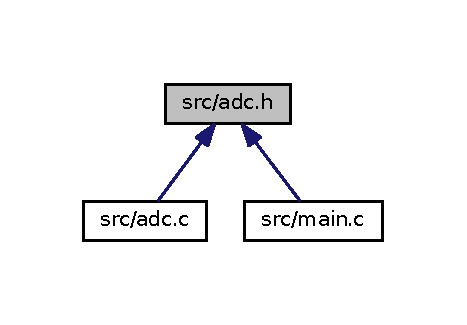
\includegraphics[width=224pt]{adc_8h__dep__incl}
\end{center}
\end{figure}
\subsection*{Classes}
\begin{DoxyCompactItemize}
\item 
struct \hyperlink{structadc__config}{adc\+\_\+config}
\item 
struct \hyperlink{structadc}{adc}
\end{DoxyCompactItemize}
\subsection*{Functions}
\begin{DoxyCompactItemize}
\item 
\hypertarget{adc_8h_a1c6689c4974ca47f5e316799961c1bab}{}void {\bfseries adc\+\_\+init} (struct \hyperlink{structadc}{adc} $\ast$\hyperlink{structadc}{adc}, enum \hyperlink{hw_8h_a3c02952100e7d051b77cdf060ca0ba9b}{hw\+\_\+init\+\_\+state} state)\label{adc_8h_a1c6689c4974ca47f5e316799961c1bab}

\item 
\hypertarget{adc_8h_ada0028bb1d8d2d158dbcdd17601f54bb}{}void {\bfseries adc\+\_\+begin\+\_\+sampling} (struct \hyperlink{structadc}{adc} $\ast$\hyperlink{structadc}{adc})\label{adc_8h_ada0028bb1d8d2d158dbcdd17601f54bb}

\end{DoxyCompactItemize}


\subsection{Detailed Description}
A\+D\+C H\+A\+L include. 


\hypertarget{dma_8c}{}\section{src/dma.c File Reference}
\label{dma_8c}\index{src/dma.\+c@{src/dma.\+c}}


D\+M\+A implementation.  


{\ttfamily \#include \char`\"{}dma.\+h\char`\"{}}\\*
Include dependency graph for dma.\+c\+:
\nopagebreak
\begin{figure}[H]
\begin{center}
\leavevmode
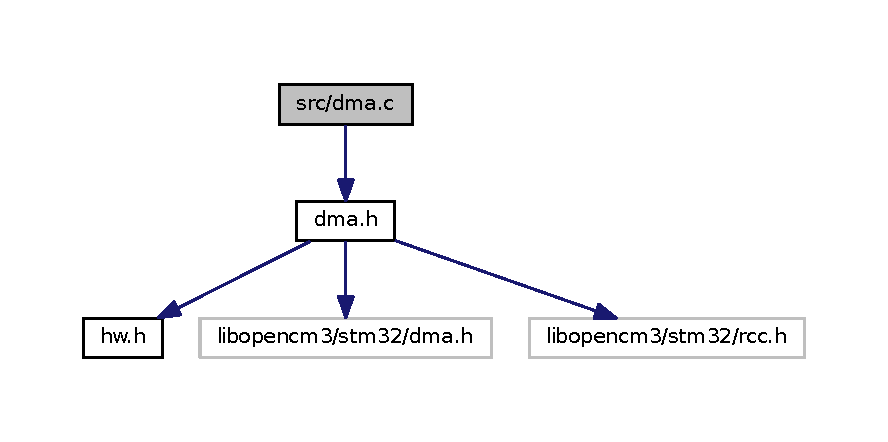
\includegraphics[width=350pt]{dma_8c__incl}
\end{center}
\end{figure}
\subsection*{Functions}
\begin{DoxyCompactItemize}
\item 
\hypertarget{dma_8c_a4dd6c4a4e3e59a2a2508cc928c2cde64}{}void {\bfseries dma\+\_\+init} (struct \hyperlink{structdma__config}{dma\+\_\+config} $\ast$dma, enum \hyperlink{hw_8h_a3c02952100e7d051b77cdf060ca0ba9b}{hw\+\_\+init\+\_\+state} state)\label{dma_8c_a4dd6c4a4e3e59a2a2508cc928c2cde64}

\item 
\hypertarget{dma_8c_aa1bc232b23b02bc61fcbcfbd0221f42f}{}void {\bfseries dma\+\_\+channel\+\_\+init} (struct \hyperlink{structdma__channel__config}{dma\+\_\+channel\+\_\+config} $\ast$channel, enum \hyperlink{hw_8h_a3c02952100e7d051b77cdf060ca0ba9b}{hw\+\_\+init\+\_\+state} state)\label{dma_8c_aa1bc232b23b02bc61fcbcfbd0221f42f}

\item 
\hypertarget{dma_8c_aea2e8fc9d6568dc073cf2a3550bf9a3a}{}void {\bfseries dma\+\_\+channel\+\_\+send} (struct \hyperlink{structdma__channel__config}{dma\+\_\+channel\+\_\+config} $\ast$channel, volatile void $\ast$data, int length)\label{dma_8c_aea2e8fc9d6568dc073cf2a3550bf9a3a}

\item 
\hypertarget{dma_8c_a5b076ef642e2110268c7757c35c2d08d}{}void {\bfseries dma\+\_\+channel\+\_\+send\+\_\+blocking} (struct \hyperlink{structdma__channel__config}{dma\+\_\+channel\+\_\+config} $\ast$channel, volatile void $\ast$data, int length)\label{dma_8c_a5b076ef642e2110268c7757c35c2d08d}

\end{DoxyCompactItemize}


\subsection{Detailed Description}
D\+M\+A implementation. 


\hypertarget{dma_8h}{}\section{src/dma.h File Reference}
\label{dma_8h}\index{src/dma.\+h@{src/dma.\+h}}


D\+M\+A includes.  


{\ttfamily \#include \char`\"{}hw.\+h\char`\"{}}\\*
{\ttfamily \#include $<$libopencm3/stm32/dma.\+h$>$}\\*
{\ttfamily \#include $<$libopencm3/stm32/rcc.\+h$>$}\\*
Include dependency graph for dma.\+h\+:
\nopagebreak
\begin{figure}[H]
\begin{center}
\leavevmode
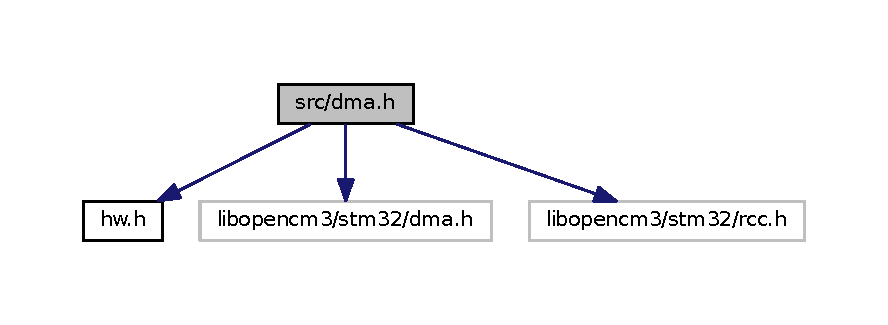
\includegraphics[width=350pt]{dma_8h__incl}
\end{center}
\end{figure}
This graph shows which files directly or indirectly include this file\+:
\nopagebreak
\begin{figure}[H]
\begin{center}
\leavevmode
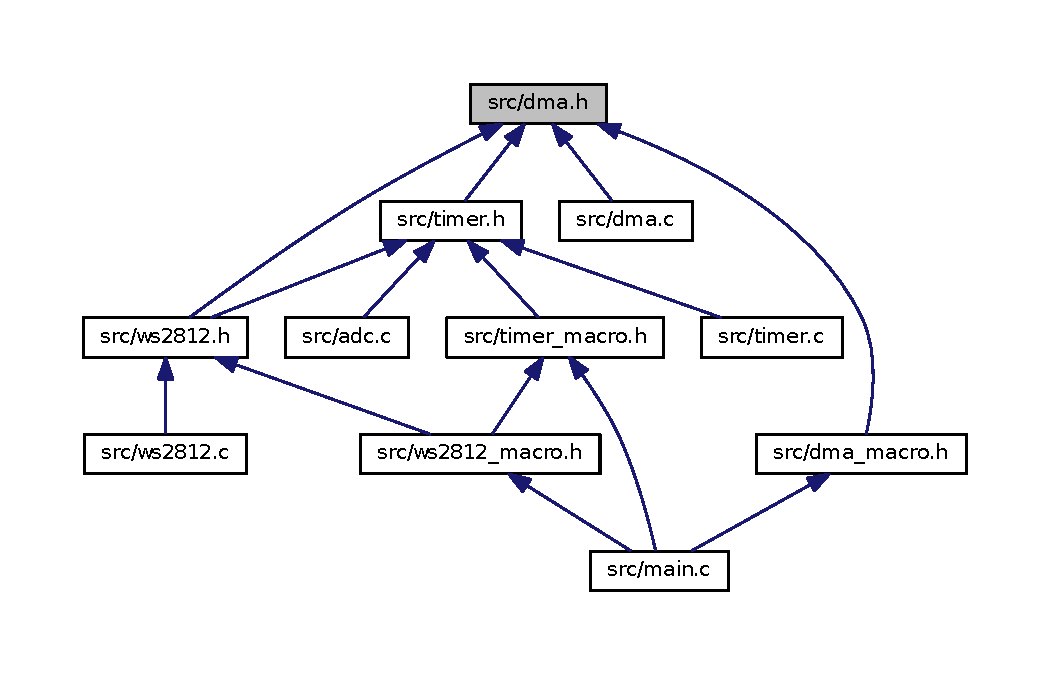
\includegraphics[width=350pt]{dma_8h__dep__incl}
\end{center}
\end{figure}
\subsection*{Classes}
\begin{DoxyCompactItemize}
\item 
struct \hyperlink{structdma__config}{dma\+\_\+config}
\item 
struct \hyperlink{structdma__channel__config}{dma\+\_\+channel\+\_\+config}
\end{DoxyCompactItemize}
\subsection*{Functions}
\begin{DoxyCompactItemize}
\item 
\hypertarget{dma_8h_a4dd6c4a4e3e59a2a2508cc928c2cde64}{}void {\bfseries dma\+\_\+init} (struct \hyperlink{structdma__config}{dma\+\_\+config} $\ast$dma, enum \hyperlink{hw_8h_a3c02952100e7d051b77cdf060ca0ba9b}{hw\+\_\+init\+\_\+state} state)\label{dma_8h_a4dd6c4a4e3e59a2a2508cc928c2cde64}

\item 
\hypertarget{dma_8h_aa1bc232b23b02bc61fcbcfbd0221f42f}{}void {\bfseries dma\+\_\+channel\+\_\+init} (struct \hyperlink{structdma__channel__config}{dma\+\_\+channel\+\_\+config} $\ast$channel, enum \hyperlink{hw_8h_a3c02952100e7d051b77cdf060ca0ba9b}{hw\+\_\+init\+\_\+state} state)\label{dma_8h_aa1bc232b23b02bc61fcbcfbd0221f42f}

\item 
\hypertarget{dma_8h_aea2e8fc9d6568dc073cf2a3550bf9a3a}{}void {\bfseries dma\+\_\+channel\+\_\+send} (struct \hyperlink{structdma__channel__config}{dma\+\_\+channel\+\_\+config} $\ast$channel, volatile void $\ast$data, int length)\label{dma_8h_aea2e8fc9d6568dc073cf2a3550bf9a3a}

\item 
\hypertarget{dma_8h_a5b076ef642e2110268c7757c35c2d08d}{}void {\bfseries dma\+\_\+channel\+\_\+send\+\_\+blocking} (struct \hyperlink{structdma__channel__config}{dma\+\_\+channel\+\_\+config} $\ast$channel, volatile void $\ast$data, int length)\label{dma_8h_a5b076ef642e2110268c7757c35c2d08d}

\end{DoxyCompactItemize}


\subsection{Detailed Description}
D\+M\+A includes. 


\hypertarget{filter_8c}{}\section{src/filter.c File Reference}
\label{filter_8c}\index{src/filter.\+c@{src/filter.\+c}}


Implementation of filter functions.  


{\ttfamily \#include \char`\"{}filter.\+h\char`\"{}}\\*
Include dependency graph for filter.\+c\+:\nopagebreak
\begin{figure}[H]
\begin{center}
\leavevmode
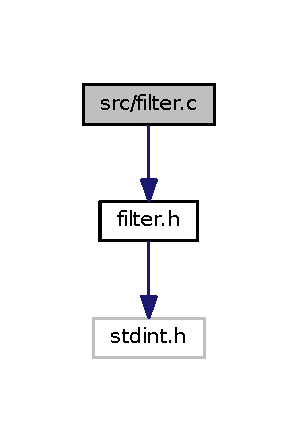
\includegraphics[width=143pt]{filter_8c__incl}
\end{center}
\end{figure}
\subsection*{Functions}
\begin{DoxyCompactItemize}
\item 
int \hyperlink{filter_8c_a8fc1140a49d6a81bfa6fb23dcce45e23}{filter\+\_\+rms\+\_\+process} (volatile struct \hyperlink{structfilter__rms}{filter\+\_\+rms} $\ast$data, int sample)
\begin{DoxyCompactList}\small\item\em Adds a sample to the filter. \end{DoxyCompactList}\end{DoxyCompactItemize}


\subsection{Detailed Description}
Implementation of filter functions. 



\subsection{Function Documentation}
\hypertarget{filter_8c_a8fc1140a49d6a81bfa6fb23dcce45e23}{}\index{filter.\+c@{filter.\+c}!filter\+\_\+rms\+\_\+process@{filter\+\_\+rms\+\_\+process}}
\index{filter\+\_\+rms\+\_\+process@{filter\+\_\+rms\+\_\+process}!filter.\+c@{filter.\+c}}
\subsubsection[{filter\+\_\+rms\+\_\+process}]{\setlength{\rightskip}{0pt plus 5cm}int filter\+\_\+rms\+\_\+process (
\begin{DoxyParamCaption}
\item[{volatile struct {\bf filter\+\_\+rms} $\ast$}]{data, }
\item[{int}]{sample}
\end{DoxyParamCaption}
)}\label{filter_8c_a8fc1140a49d6a81bfa6fb23dcce45e23}


Adds a sample to the filter. 


\begin{DoxyParams}{Parameters}
{\em data} & Filter state \\
\hline
{\em sample} & New sample \\
\hline
\end{DoxyParams}
\begin{DoxyReturn}{Returns}
Filtered result if possible, otherwise -\/1 
\end{DoxyReturn}


Definition at line 11 of file filter.\+c.



References filter\+\_\+rms\+::count, filter\+\_\+rms\+::invalid\+\_\+samples\+\_\+streak, filter\+\_\+rms\+::pos, filter\+\_\+rms\+::size, and filter\+\_\+rms\+::sqsum.


\hypertarget{filter_8h}{}\section{src/filter.h File Reference}
\label{filter_8h}\index{src/filter.\+h@{src/filter.\+h}}


Filter functions for filtering sensor data.  


{\ttfamily \#include $<$stdint.\+h$>$}\\*
Include dependency graph for filter.\+h\+:\nopagebreak
\begin{figure}[H]
\begin{center}
\leavevmode
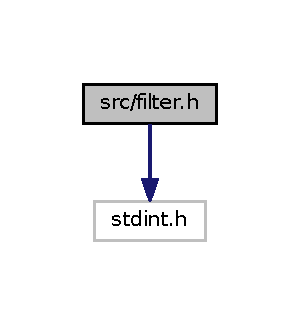
\includegraphics[width=144pt]{filter_8h__incl}
\end{center}
\end{figure}
This graph shows which files directly or indirectly include this file\+:\nopagebreak
\begin{figure}[H]
\begin{center}
\leavevmode
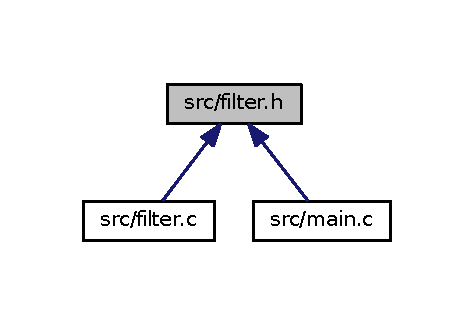
\includegraphics[width=228pt]{filter_8h__dep__incl}
\end{center}
\end{figure}
\subsection*{Classes}
\begin{DoxyCompactItemize}
\item 
struct \hyperlink{structfilter__sample__range}{filter\+\_\+sample\+\_\+range}
\begin{DoxyCompactList}\small\item\em A valid range for samples. \end{DoxyCompactList}\item 
struct \hyperlink{structfilter__rms}{filter\+\_\+rms}
\begin{DoxyCompactList}\small\item\em R\+M\+S filter configuration and state. \end{DoxyCompactList}\end{DoxyCompactItemize}
\subsection*{Functions}
\begin{DoxyCompactItemize}
\item 
int \hyperlink{filter_8h_a8fc1140a49d6a81bfa6fb23dcce45e23}{filter\+\_\+rms\+\_\+process} (volatile struct \hyperlink{structfilter__rms}{filter\+\_\+rms} $\ast$data, int sample)
\begin{DoxyCompactList}\small\item\em Adds a sample to the filter. \end{DoxyCompactList}\end{DoxyCompactItemize}


\subsection{Detailed Description}
Filter functions for filtering sensor data. 



\subsection{Function Documentation}
\hypertarget{filter_8h_a8fc1140a49d6a81bfa6fb23dcce45e23}{}\index{filter.\+h@{filter.\+h}!filter\+\_\+rms\+\_\+process@{filter\+\_\+rms\+\_\+process}}
\index{filter\+\_\+rms\+\_\+process@{filter\+\_\+rms\+\_\+process}!filter.\+h@{filter.\+h}}
\subsubsection[{filter\+\_\+rms\+\_\+process}]{\setlength{\rightskip}{0pt plus 5cm}int filter\+\_\+rms\+\_\+process (
\begin{DoxyParamCaption}
\item[{volatile struct {\bf filter\+\_\+rms} $\ast$}]{data, }
\item[{int}]{sample}
\end{DoxyParamCaption}
)}\label{filter_8h_a8fc1140a49d6a81bfa6fb23dcce45e23}


Adds a sample to the filter. 


\begin{DoxyParams}{Parameters}
{\em data} & Filter state \\
\hline
{\em sample} & New sample \\
\hline
\end{DoxyParams}
\begin{DoxyReturn}{Returns}
Filtered result if possible, otherwise -\/1 
\end{DoxyReturn}


Definition at line 11 of file filter.\+c.



References filter\+\_\+rms\+::count, filter\+\_\+rms\+::invalid\+\_\+samples\+\_\+streak, filter\+\_\+rms\+::pos, filter\+\_\+rms\+::size, and filter\+\_\+rms\+::sqsum.


\hypertarget{gpio_8c}{}\section{src/gpio.c File Reference}
\label{gpio_8c}\index{src/gpio.\+c@{src/gpio.\+c}}


G\+P\+I\+O H\+A\+L implementation.  


{\ttfamily \#include \char`\"{}gpio.\+h\char`\"{}}\\*
Include dependency graph for gpio.\+c\+:\nopagebreak
\begin{figure}[H]
\begin{center}
\leavevmode
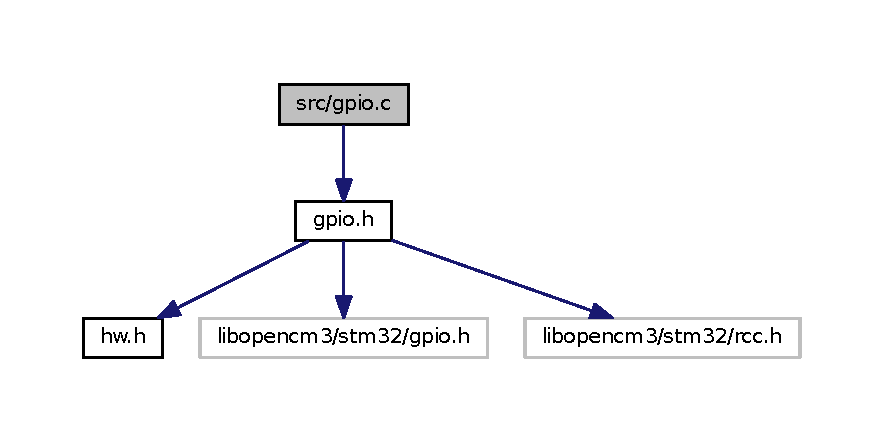
\includegraphics[width=350pt]{gpio_8c__incl}
\end{center}
\end{figure}
\subsection*{Functions}
\begin{DoxyCompactItemize}
\item 
\hypertarget{gpio_8c_a63bdba86b81c90cc95acc241a940bf43}{}void {\bfseries gpio\+\_\+port\+\_\+init} (struct \hyperlink{structgpio__port}{gpio\+\_\+port} $\ast$port, enum \hyperlink{hw_8h_a3c02952100e7d051b77cdf060ca0ba9b}{hw\+\_\+init\+\_\+state} state)\label{gpio_8c_a63bdba86b81c90cc95acc241a940bf43}

\item 
\hypertarget{gpio_8c_ac75279cf93c1946e67efa99e33d32569}{}void {\bfseries gpio\+\_\+pin\+\_\+init} (struct \hyperlink{structgpio__pin}{gpio\+\_\+pin} $\ast$pin, enum \hyperlink{hw_8h_a3c02952100e7d051b77cdf060ca0ba9b}{hw\+\_\+init\+\_\+state} state)\label{gpio_8c_ac75279cf93c1946e67efa99e33d32569}

\end{DoxyCompactItemize}


\subsection{Detailed Description}
G\+P\+I\+O H\+A\+L implementation. 


\hypertarget{gpio_8h}{}\section{src/gpio.h File Reference}
\label{gpio_8h}\index{src/gpio.\+h@{src/gpio.\+h}}


G\+P\+I\+O H\+A\+L includes.  


{\ttfamily \#include \char`\"{}hw.\+h\char`\"{}}\\*
{\ttfamily \#include $<$libopencm3/stm32/gpio.\+h$>$}\\*
{\ttfamily \#include $<$libopencm3/stm32/rcc.\+h$>$}\\*
Include dependency graph for gpio.\+h\+:\nopagebreak
\begin{figure}[H]
\begin{center}
\leavevmode
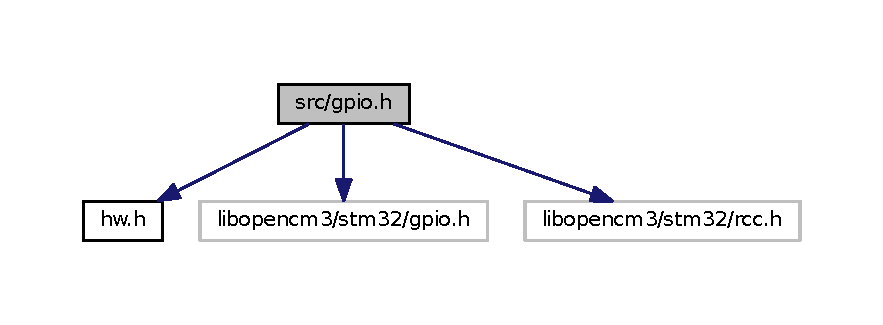
\includegraphics[width=350pt]{gpio_8h__incl}
\end{center}
\end{figure}
This graph shows which files directly or indirectly include this file\+:\nopagebreak
\begin{figure}[H]
\begin{center}
\leavevmode
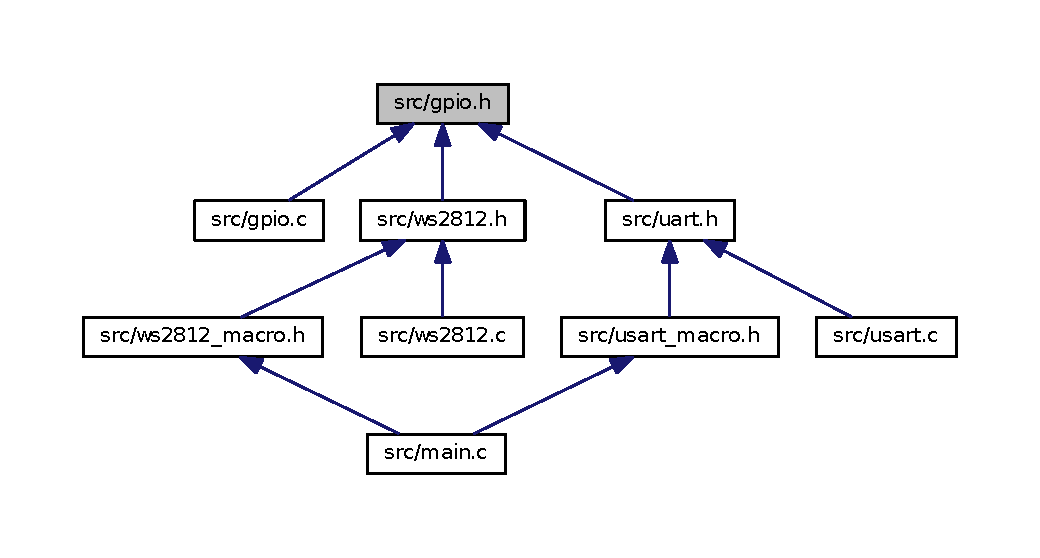
\includegraphics[width=350pt]{gpio_8h__dep__incl}
\end{center}
\end{figure}
\subsection*{Classes}
\begin{DoxyCompactItemize}
\item 
struct \hyperlink{structgpio__port}{gpio\+\_\+port}
\item 
struct \hyperlink{structgpio__port__config}{gpio\+\_\+port\+\_\+config}
\item 
struct \hyperlink{structgpio__pin__config}{gpio\+\_\+pin\+\_\+config}
\item 
struct \hyperlink{structgpio__pin}{gpio\+\_\+pin}
\end{DoxyCompactItemize}
\subsection*{Functions}
\begin{DoxyCompactItemize}
\item 
\hypertarget{gpio_8h_ac75279cf93c1946e67efa99e33d32569}{}void {\bfseries gpio\+\_\+pin\+\_\+init} (struct \hyperlink{structgpio__pin}{gpio\+\_\+pin} $\ast$pin, enum \hyperlink{hw_8h_a3c02952100e7d051b77cdf060ca0ba9b}{hw\+\_\+init\+\_\+state} state)\label{gpio_8h_ac75279cf93c1946e67efa99e33d32569}

\item 
\hypertarget{gpio_8h_a15b8abcad7353c21ecd2f8bb0f5dee02}{}void {\bfseries gpio\+\_\+port\+\_\+init} (struct \hyperlink{structgpio__port}{gpio\+\_\+port} $\ast$pin, enum \hyperlink{hw_8h_a3c02952100e7d051b77cdf060ca0ba9b}{hw\+\_\+init\+\_\+state} state)\label{gpio_8h_a15b8abcad7353c21ecd2f8bb0f5dee02}

\end{DoxyCompactItemize}


\subsection{Detailed Description}
G\+P\+I\+O H\+A\+L includes. 


\hypertarget{gpio__macro_8h}{}\section{src/gpio\+\_\+macro.h File Reference}
\label{gpio__macro_8h}\index{src/gpio\+\_\+macro.\+h@{src/gpio\+\_\+macro.\+h}}


Helper macros for G\+P\+I\+O.  


This graph shows which files directly or indirectly include this file\+:\nopagebreak
\begin{figure}[H]
\begin{center}
\leavevmode
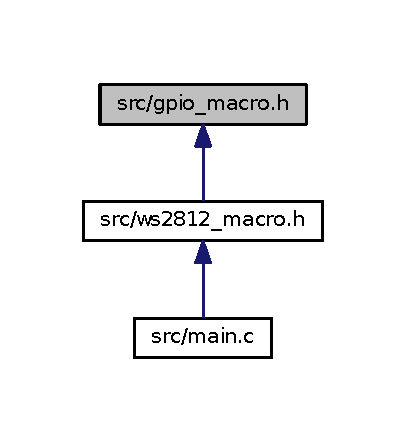
\includegraphics[width=195pt]{gpio__macro_8h__dep__incl}
\end{center}
\end{figure}
\subsection*{Macros}
\begin{DoxyCompactItemize}
\item 
\#define \hyperlink{gpio__macro_8h_aecbaaaba532fce90bdbb37ff13fa220e}{G\+P\+I\+O\+\_\+\+P\+O\+R\+T\+\_\+\+I\+N\+S\+T\+A\+N\+C\+E}(Name,  Port,  Rcc)
\begin{DoxyCompactList}\small\item\em Declares a new G\+P\+I\+O port. \end{DoxyCompactList}\item 
\#define \hyperlink{gpio__macro_8h_ac93174a4de27900671c09ea62ffb16b2}{G\+P\+I\+O\+\_\+\+P\+I\+N\+\_\+\+I\+N\+S\+T\+A\+N\+C\+E}(Name,  Port,  Mode,  Configuration,  Pin)
\begin{DoxyCompactList}\small\item\em Declares a new G\+P\+I\+O pin and G\+P\+I\+O pin config. \end{DoxyCompactList}\item 
\#define \hyperlink{gpio__macro_8h_a1b2ea2f540968f79ec27781d05350843}{G\+P\+I\+O\+\_\+\+P\+I\+N\+\_\+\+N\+O\+C\+O\+N\+F}(Name,  Port,  Pin)~\hyperlink{gpio__macro_8h_ac93174a4de27900671c09ea62ffb16b2}{G\+P\+I\+O\+\_\+\+P\+I\+N\+\_\+\+I\+N\+S\+T\+A\+N\+C\+E}(Name, Port, 0, 0, Pin)
\begin{DoxyCompactList}\small\item\em Create G\+P\+I\+O pin with no configuration. \end{DoxyCompactList}\item 
\hypertarget{gpio__macro_8h_a799ae7b1d569950c8d113d31e5c98ebf}{}\#define {\bfseries \+\_\+\+G\+P\+I\+O\+\_\+\+M\+A\+C\+R\+O\+\_\+\+H\+\_\+}\label{gpio__macro_8h_a799ae7b1d569950c8d113d31e5c98ebf}

\end{DoxyCompactItemize}


\subsection{Detailed Description}
Helper macros for G\+P\+I\+O. 



\subsection{Macro Definition Documentation}
\hypertarget{gpio__macro_8h_ac93174a4de27900671c09ea62ffb16b2}{}\index{gpio\+\_\+macro.\+h@{gpio\+\_\+macro.\+h}!G\+P\+I\+O\+\_\+\+P\+I\+N\+\_\+\+I\+N\+S\+T\+A\+N\+C\+E@{G\+P\+I\+O\+\_\+\+P\+I\+N\+\_\+\+I\+N\+S\+T\+A\+N\+C\+E}}
\index{G\+P\+I\+O\+\_\+\+P\+I\+N\+\_\+\+I\+N\+S\+T\+A\+N\+C\+E@{G\+P\+I\+O\+\_\+\+P\+I\+N\+\_\+\+I\+N\+S\+T\+A\+N\+C\+E}!gpio\+\_\+macro.\+h@{gpio\+\_\+macro.\+h}}
\subsubsection[{G\+P\+I\+O\+\_\+\+P\+I\+N\+\_\+\+I\+N\+S\+T\+A\+N\+C\+E}]{\setlength{\rightskip}{0pt plus 5cm}\#define G\+P\+I\+O\+\_\+\+P\+I\+N\+\_\+\+I\+N\+S\+T\+A\+N\+C\+E(
\begin{DoxyParamCaption}
\item[{}]{Name, }
\item[{}]{Port, }
\item[{}]{Mode, }
\item[{}]{Configuration, }
\item[{}]{Pin}
\end{DoxyParamCaption}
)}\label{gpio__macro_8h_ac93174a4de27900671c09ea62ffb16b2}
{\bfseries Value\+:}
\begin{DoxyCode}
\textcolor{keyword}{struct }\hyperlink{structgpio__pin__config}{gpio\_pin\_config} Name##\_config = \{\(\backslash\)
    .port = Port,\(\backslash\)
    .mode = Mode,\(\backslash\)
    .configuration = Configuration,\(\backslash\)
    .pin = Pin,\(\backslash\)
\};\(\backslash\)
\(\backslash\)
struct \hyperlink{structgpio__pin}{gpio\_pin} Name = \{\(\backslash\)
    .configuration = &Name##\_config,\(\backslash\)
\};
\end{DoxyCode}


Declares a new G\+P\+I\+O pin and G\+P\+I\+O pin config. 


\begin{DoxyParams}{Parameters}
{\em Name} & Variable name \\
\hline
{\em Port} & Pointer to struct \hyperlink{structgpio__port}{gpio\+\_\+port} to use \\
\hline
{\em Mode} & The G\+P\+I\+O pin mode \\
\hline
{\em Configuration} & The G\+P\+I\+O pin configuration \\
\hline
{\em Pin} & The G\+P\+I\+O pin mask \\
\hline
\end{DoxyParams}
\begin{DoxyReturn}{Returns}
struct \hyperlink{structgpio__pin__config}{gpio\+\_\+pin\+\_\+config} Name\+\_\+config ~\newline
 struct \hyperlink{structgpio__pin}{gpio\+\_\+pin} Name 
\end{DoxyReturn}


Definition at line 33 of file gpio\+\_\+macro.\+h.

\hypertarget{gpio__macro_8h_a1b2ea2f540968f79ec27781d05350843}{}\index{gpio\+\_\+macro.\+h@{gpio\+\_\+macro.\+h}!G\+P\+I\+O\+\_\+\+P\+I\+N\+\_\+\+N\+O\+C\+O\+N\+F@{G\+P\+I\+O\+\_\+\+P\+I\+N\+\_\+\+N\+O\+C\+O\+N\+F}}
\index{G\+P\+I\+O\+\_\+\+P\+I\+N\+\_\+\+N\+O\+C\+O\+N\+F@{G\+P\+I\+O\+\_\+\+P\+I\+N\+\_\+\+N\+O\+C\+O\+N\+F}!gpio\+\_\+macro.\+h@{gpio\+\_\+macro.\+h}}
\subsubsection[{G\+P\+I\+O\+\_\+\+P\+I\+N\+\_\+\+N\+O\+C\+O\+N\+F}]{\setlength{\rightskip}{0pt plus 5cm}\#define G\+P\+I\+O\+\_\+\+P\+I\+N\+\_\+\+N\+O\+C\+O\+N\+F(
\begin{DoxyParamCaption}
\item[{}]{Name, }
\item[{}]{Port, }
\item[{}]{Pin}
\end{DoxyParamCaption}
)~{\bf G\+P\+I\+O\+\_\+\+P\+I\+N\+\_\+\+I\+N\+S\+T\+A\+N\+C\+E}(Name, Port, 0, 0, Pin)}\label{gpio__macro_8h_a1b2ea2f540968f79ec27781d05350843}


Create G\+P\+I\+O pin with no configuration. 



Definition at line 46 of file gpio\+\_\+macro.\+h.

\hypertarget{gpio__macro_8h_aecbaaaba532fce90bdbb37ff13fa220e}{}\index{gpio\+\_\+macro.\+h@{gpio\+\_\+macro.\+h}!G\+P\+I\+O\+\_\+\+P\+O\+R\+T\+\_\+\+I\+N\+S\+T\+A\+N\+C\+E@{G\+P\+I\+O\+\_\+\+P\+O\+R\+T\+\_\+\+I\+N\+S\+T\+A\+N\+C\+E}}
\index{G\+P\+I\+O\+\_\+\+P\+O\+R\+T\+\_\+\+I\+N\+S\+T\+A\+N\+C\+E@{G\+P\+I\+O\+\_\+\+P\+O\+R\+T\+\_\+\+I\+N\+S\+T\+A\+N\+C\+E}!gpio\+\_\+macro.\+h@{gpio\+\_\+macro.\+h}}
\subsubsection[{G\+P\+I\+O\+\_\+\+P\+O\+R\+T\+\_\+\+I\+N\+S\+T\+A\+N\+C\+E}]{\setlength{\rightskip}{0pt plus 5cm}\#define G\+P\+I\+O\+\_\+\+P\+O\+R\+T\+\_\+\+I\+N\+S\+T\+A\+N\+C\+E(
\begin{DoxyParamCaption}
\item[{}]{Name, }
\item[{}]{Port, }
\item[{}]{Rcc}
\end{DoxyParamCaption}
)}\label{gpio__macro_8h_aecbaaaba532fce90bdbb37ff13fa220e}
{\bfseries Value\+:}
\begin{DoxyCode}
\textcolor{keyword}{struct }\hyperlink{structgpio__port}{gpio\_port} Name = \{\(\backslash\)
    .configuration = &((\textcolor{keyword}{struct }\hyperlink{structgpio__port__config}{gpio\_port\_config})\{\(\backslash\)
        .port = Port,\(\backslash\)
        .rcc = Rcc,\(\backslash\)
    \}),\(\backslash\)
\};
\end{DoxyCode}


Declares a new G\+P\+I\+O port. 


\begin{DoxyParams}{Parameters}
{\em Name} & Variable name \\
\hline
{\em Port} & The G\+P\+I\+O port base address \\
\hline
{\em Rcc} & The R\+C\+C index \\
\hline
\end{DoxyParams}
\begin{DoxyReturn}{Returns}
struct \hyperlink{structgpio__port}{gpio\+\_\+port} Name 
\end{DoxyReturn}


Definition at line 14 of file gpio\+\_\+macro.\+h.


\hypertarget{hw_8c}{}\section{src/hw.c File Reference}
\label{hw_8c}\index{src/hw.\+c@{src/hw.\+c}}


H\+A\+L main control.  


{\ttfamily \#include \char`\"{}hw.\+h\char`\"{}}\\*
Include dependency graph for hw.\+c\+:\nopagebreak
\begin{figure}[H]
\begin{center}
\leavevmode
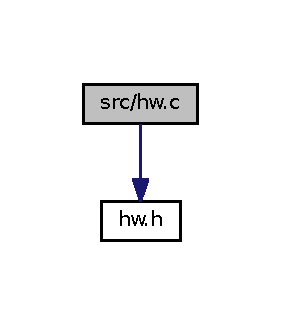
\includegraphics[width=135pt]{hw_8c__incl}
\end{center}
\end{figure}
\subsection*{Functions}
\begin{DoxyCompactItemize}
\item 
void \hyperlink{hw_8c_acf938165e604a675fe09218a1b3cfb5f}{hw\+\_\+init} ()
\begin{DoxyCompactList}\small\item\em Call hw\+\_\+init\+\_\+state with all states to go trough. \end{DoxyCompactList}\end{DoxyCompactItemize}


\subsection{Detailed Description}
H\+A\+L main control. 



\subsection{Function Documentation}
\hypertarget{hw_8c_acf938165e604a675fe09218a1b3cfb5f}{}\index{hw.\+c@{hw.\+c}!hw\+\_\+init@{hw\+\_\+init}}
\index{hw\+\_\+init@{hw\+\_\+init}!hw.\+c@{hw.\+c}}
\subsubsection[{hw\+\_\+init}]{\setlength{\rightskip}{0pt plus 5cm}void hw\+\_\+init (
\begin{DoxyParamCaption}
{}
\end{DoxyParamCaption}
)}\label{hw_8c_acf938165e604a675fe09218a1b3cfb5f}


Call hw\+\_\+init\+\_\+state with all states to go trough. 



Definition at line 18 of file hw.\+c.



References H\+W\+\_\+\+I\+N\+I\+T\+\_\+\+G\+P\+I\+O, H\+W\+\_\+\+I\+N\+I\+T\+\_\+\+N\+V\+I\+C, H\+W\+\_\+\+I\+N\+I\+T\+\_\+\+P\+O\+S\+T\+\_\+\+I\+N\+I\+T, H\+W\+\_\+\+I\+N\+I\+T\+\_\+\+P\+R\+E\+\_\+\+N\+V\+I\+C, and H\+W\+\_\+\+I\+N\+I\+T\+\_\+\+R\+C\+C.



Referenced by main().


\hypertarget{hw_8h}{}\section{src/hw.h File Reference}
\label{hw_8h}\index{src/hw.\+h@{src/hw.\+h}}


Hardware abstraction layer include file.  


This graph shows which files directly or indirectly include this file\+:\nopagebreak
\begin{figure}[H]
\begin{center}
\leavevmode
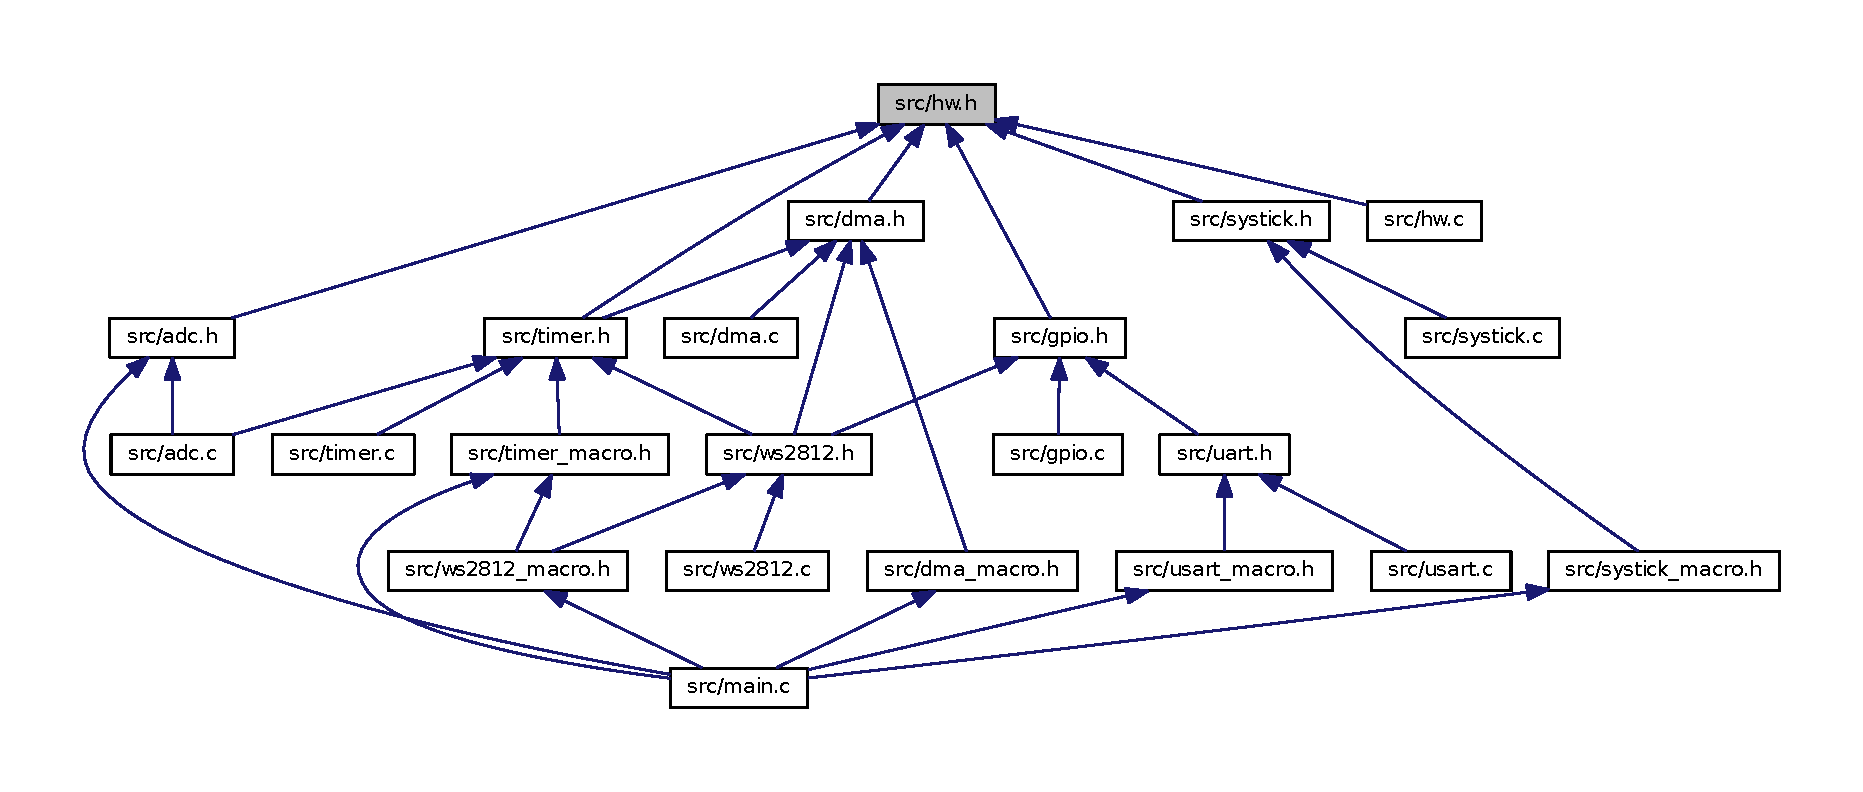
\includegraphics[width=350pt]{hw_8h__dep__incl}
\end{center}
\end{figure}
\subsection*{Macros}
\begin{DoxyCompactItemize}
\item 
\#define \hyperlink{hw_8h_a40deaf267e014e0489a474b8eb6f7378}{D\+E\+F\+A\+U\+L\+T}(value,  default)~value = value ? value \+: default
\begin{DoxyCompactList}\small\item\em Sets a value if the value evaluates to false. \end{DoxyCompactList}\item 
\hypertarget{hw_8h_a2c9e85d22a9ba37ea589b1747af46307}{}\#define {\bfseries V\+R\+E\+F}~3.\+295\label{hw_8h_a2c9e85d22a9ba37ea589b1747af46307}

\item 
\hypertarget{hw_8h_a918f64eb53db8e8dc694f36a87646476}{}\#define {\bfseries R1}~100000.\+0\label{hw_8h_a918f64eb53db8e8dc694f36a87646476}

\item 
\hypertarget{hw_8h_aa6d350d439222376ecc6da4bb50403c2}{}\#define {\bfseries N\+T\+C\+\_\+\+R}~150000\label{hw_8h_aa6d350d439222376ecc6da4bb50403c2}

\item 
\hypertarget{hw_8h_a18525dcee03997cc094fdf30c82fbf1c}{}\#define {\bfseries N\+T\+C\+\_\+\+A1}~3.\+354016\+E-\/03\label{hw_8h_a18525dcee03997cc094fdf30c82fbf1c}

\item 
\hypertarget{hw_8h_a203d2ab7a8a9a70d5455888b923d341b}{}\#define {\bfseries N\+T\+C\+\_\+\+B1}~2.\+367720\+E-\/04\label{hw_8h_a203d2ab7a8a9a70d5455888b923d341b}

\item 
\hypertarget{hw_8h_ab9a7131a2fb1b8f70f428e5198ada9c1}{}\#define {\bfseries N\+T\+C\+\_\+\+C1}~3.\+585140\+E-\/06\label{hw_8h_ab9a7131a2fb1b8f70f428e5198ada9c1}

\item 
\hypertarget{hw_8h_aecc61ee6e79b14087f05cd59f8252898}{}\#define {\bfseries N\+T\+C\+\_\+\+D1}~1.\+255349\+E-\/07\label{hw_8h_aecc61ee6e79b14087f05cd59f8252898}

\item 
\hypertarget{hw_8h_a16b6412d50d047f1699f6882b7166d24}{}\#define {\bfseries T0\+\_\+\+K}~273.\+15\label{hw_8h_a16b6412d50d047f1699f6882b7166d24}

\item 
\hypertarget{hw_8h_aacaca0988244bd3a888ca5befa89f44b}{}\#define {\bfseries P\+W\+M\+\_\+\+P\+E\+R\+I\+O\+D}~4096\label{hw_8h_aacaca0988244bd3a888ca5befa89f44b}

\item 
\hypertarget{hw_8h_a0565d8b2c16056c3a4d9f916a7fe2ef3}{}\#define {\bfseries P\+W\+M\+\_\+\+T\+O\+P}~(P\+W\+M\+\_\+\+P\+E\+R\+I\+O\+D -\/ 1)\label{hw_8h_a0565d8b2c16056c3a4d9f916a7fe2ef3}

\item 
\hypertarget{hw_8h_aad6d4d2ba34b16b7fa27f303d506ef71}{}\#define {\bfseries \+\_\+\+H\+W\+\_\+\+H\+\_\+}\label{hw_8h_aad6d4d2ba34b16b7fa27f303d506ef71}

\end{DoxyCompactItemize}
\subsection*{Enumerations}
\begin{DoxyCompactItemize}
\item 
enum \hyperlink{hw_8h_a3c02952100e7d051b77cdf060ca0ba9b}{hw\+\_\+init\+\_\+state} \{ \\*
\hyperlink{hw_8h_a3c02952100e7d051b77cdf060ca0ba9ba6b96182ed0808ff30887f91b24d86849}{H\+W\+\_\+\+I\+N\+I\+T\+\_\+\+U\+N\+I\+N\+I\+T\+I\+A\+L\+I\+Z\+E\+D}, 
\hyperlink{hw_8h_a3c02952100e7d051b77cdf060ca0ba9baca0b4dbf0e3911b3edde56d700f76ecf}{H\+W\+\_\+\+I\+N\+I\+T\+\_\+\+R\+C\+C}, 
\hyperlink{hw_8h_a3c02952100e7d051b77cdf060ca0ba9ba4e9b2d4b7e946d95c2e41f3de17035a0}{H\+W\+\_\+\+I\+N\+I\+T\+\_\+\+G\+P\+I\+O}, 
\hyperlink{hw_8h_a3c02952100e7d051b77cdf060ca0ba9ba45012c00c17031e71a4f60ada04df07d}{H\+W\+\_\+\+I\+N\+I\+T\+\_\+\+P\+R\+E\+\_\+\+N\+V\+I\+C}, 
\\*
\hyperlink{hw_8h_a3c02952100e7d051b77cdf060ca0ba9ba3f137ea5dd6b2ac372bb6d175434b3fa}{H\+W\+\_\+\+I\+N\+I\+T\+\_\+\+N\+V\+I\+C}, 
\hyperlink{hw_8h_a3c02952100e7d051b77cdf060ca0ba9bacf9b04dc351d9fc47482fcd5229eb201}{H\+W\+\_\+\+I\+N\+I\+T\+\_\+\+P\+O\+S\+T\+\_\+\+I\+N\+I\+T}, 
{\bfseries H\+W\+\_\+\+I\+N\+I\+T\+\_\+\+I\+N\+I\+T\+I\+A\+L\+I\+Z\+E\+D}
 \}
\begin{DoxyCompactList}\small\item\em This is the state of the hardware abstraction layer. \end{DoxyCompactList}\end{DoxyCompactItemize}
\subsection*{Functions}
\begin{DoxyCompactItemize}
\item 
void \hyperlink{hw_8h_acf938165e604a675fe09218a1b3cfb5f}{hw\+\_\+init} ()
\begin{DoxyCompactList}\small\item\em Call hw\+\_\+init\+\_\+state with all states to go trough. \end{DoxyCompactList}\item 
void \hyperlink{hw_8h_aabae29cd362c0001a2b417c9206cb330}{hw\+\_\+init\+\_\+state} (enum \hyperlink{hw_8h_a3c02952100e7d051b77cdf060ca0ba9b}{hw\+\_\+init\+\_\+state} state)
\begin{DoxyCompactList}\small\item\em This function prototype calls all perhipherals with the state as argument. \end{DoxyCompactList}\end{DoxyCompactItemize}


\subsection{Detailed Description}
Hardware abstraction layer include file. 

\begin{DoxyRefDesc}{Todo}
\item[\hyperlink{todo__todo000001}{Todo}]There is some stuff not belonging to this file in here, it should be moved\end{DoxyRefDesc}


The hardware abstraction layer should be completely generic except that it initializes the system in a predefined order 

\subsection{Macro Definition Documentation}
\hypertarget{hw_8h_a40deaf267e014e0489a474b8eb6f7378}{}\index{hw.\+h@{hw.\+h}!D\+E\+F\+A\+U\+L\+T@{D\+E\+F\+A\+U\+L\+T}}
\index{D\+E\+F\+A\+U\+L\+T@{D\+E\+F\+A\+U\+L\+T}!hw.\+h@{hw.\+h}}
\subsubsection[{D\+E\+F\+A\+U\+L\+T}]{\setlength{\rightskip}{0pt plus 5cm}\#define D\+E\+F\+A\+U\+L\+T(
\begin{DoxyParamCaption}
\item[{}]{value, }
\item[{}]{default}
\end{DoxyParamCaption}
)~value = value ? value \+: default}\label{hw_8h_a40deaf267e014e0489a474b8eb6f7378}


Sets a value if the value evaluates to false. 


\begin{DoxyParams}{Parameters}
{\em value} & Variable to check and possibly set \\
\hline
{\em default} & Default value if value was 0 \\
\hline
\end{DoxyParams}


Definition at line 15 of file hw.\+h.



Referenced by timer\+\_\+ccr\+\_\+init(), usart\+\_\+configure\+\_\+gpio(), usart\+\_\+set\+\_\+defaults(), ws2812\+\_\+configure\+\_\+gpio(), ws2812\+\_\+configure\+\_\+timer(), and ws2812\+\_\+set\+\_\+defaults().



\subsection{Enumeration Type Documentation}
\hypertarget{hw_8h_a3c02952100e7d051b77cdf060ca0ba9b}{}\index{hw.\+h@{hw.\+h}!hw\+\_\+init\+\_\+state@{hw\+\_\+init\+\_\+state}}
\index{hw\+\_\+init\+\_\+state@{hw\+\_\+init\+\_\+state}!hw.\+h@{hw.\+h}}
\subsubsection[{hw\+\_\+init\+\_\+state}]{\setlength{\rightskip}{0pt plus 5cm}enum {\bf hw\+\_\+init\+\_\+state}}\label{hw_8h_a3c02952100e7d051b77cdf060ca0ba9b}


This is the state of the hardware abstraction layer. 

\begin{Desc}
\item[Enumerator]\par
\begin{description}
\index{H\+W\+\_\+\+I\+N\+I\+T\+\_\+\+U\+N\+I\+N\+I\+T\+I\+A\+L\+I\+Z\+E\+D@{H\+W\+\_\+\+I\+N\+I\+T\+\_\+\+U\+N\+I\+N\+I\+T\+I\+A\+L\+I\+Z\+E\+D}!hw.\+h@{hw.\+h}}\index{hw.\+h@{hw.\+h}!H\+W\+\_\+\+I\+N\+I\+T\+\_\+\+U\+N\+I\+N\+I\+T\+I\+A\+L\+I\+Z\+E\+D@{H\+W\+\_\+\+I\+N\+I\+T\+\_\+\+U\+N\+I\+N\+I\+T\+I\+A\+L\+I\+Z\+E\+D}}\item[{\em 
\hypertarget{hw_8h_a3c02952100e7d051b77cdf060ca0ba9ba6b96182ed0808ff30887f91b24d86849}{}H\+W\+\_\+\+I\+N\+I\+T\+\_\+\+U\+N\+I\+N\+I\+T\+I\+A\+L\+I\+Z\+E\+D\label{hw_8h_a3c02952100e7d051b77cdf060ca0ba9ba6b96182ed0808ff30887f91b24d86849}
}]Hardware is not initialized. \index{H\+W\+\_\+\+I\+N\+I\+T\+\_\+\+R\+C\+C@{H\+W\+\_\+\+I\+N\+I\+T\+\_\+\+R\+C\+C}!hw.\+h@{hw.\+h}}\index{hw.\+h@{hw.\+h}!H\+W\+\_\+\+I\+N\+I\+T\+\_\+\+R\+C\+C@{H\+W\+\_\+\+I\+N\+I\+T\+\_\+\+R\+C\+C}}\item[{\em 
\hypertarget{hw_8h_a3c02952100e7d051b77cdf060ca0ba9baca0b4dbf0e3911b3edde56d700f76ecf}{}H\+W\+\_\+\+I\+N\+I\+T\+\_\+\+R\+C\+C\label{hw_8h_a3c02952100e7d051b77cdf060ca0ba9baca0b4dbf0e3911b3edde56d700f76ecf}
}]This is the first state entered and here hardware drivers may initialize any clocks needed. \index{H\+W\+\_\+\+I\+N\+I\+T\+\_\+\+G\+P\+I\+O@{H\+W\+\_\+\+I\+N\+I\+T\+\_\+\+G\+P\+I\+O}!hw.\+h@{hw.\+h}}\index{hw.\+h@{hw.\+h}!H\+W\+\_\+\+I\+N\+I\+T\+\_\+\+G\+P\+I\+O@{H\+W\+\_\+\+I\+N\+I\+T\+\_\+\+G\+P\+I\+O}}\item[{\em 
\hypertarget{hw_8h_a3c02952100e7d051b77cdf060ca0ba9ba4e9b2d4b7e946d95c2e41f3de17035a0}{}H\+W\+\_\+\+I\+N\+I\+T\+\_\+\+G\+P\+I\+O\label{hw_8h_a3c02952100e7d051b77cdf060ca0ba9ba4e9b2d4b7e946d95c2e41f3de17035a0}
}]After clocks have been initialized all G\+P\+I\+O will be initialized, this also puts pins to their default value) \index{H\+W\+\_\+\+I\+N\+I\+T\+\_\+\+P\+R\+E\+\_\+\+N\+V\+I\+C@{H\+W\+\_\+\+I\+N\+I\+T\+\_\+\+P\+R\+E\+\_\+\+N\+V\+I\+C}!hw.\+h@{hw.\+h}}\index{hw.\+h@{hw.\+h}!H\+W\+\_\+\+I\+N\+I\+T\+\_\+\+P\+R\+E\+\_\+\+N\+V\+I\+C@{H\+W\+\_\+\+I\+N\+I\+T\+\_\+\+P\+R\+E\+\_\+\+N\+V\+I\+C}}\item[{\em 
\hypertarget{hw_8h_a3c02952100e7d051b77cdf060ca0ba9ba45012c00c17031e71a4f60ada04df07d}{}H\+W\+\_\+\+I\+N\+I\+T\+\_\+\+P\+R\+E\+\_\+\+N\+V\+I\+C\label{hw_8h_a3c02952100e7d051b77cdf060ca0ba9ba45012c00c17031e71a4f60ada04df07d}
}]After G\+P\+I\+Os have been initialized we might want to do some stuff before N\+V\+I\+C. \begin{DoxyRefDesc}{Todo}
\item[\hyperlink{todo__todo000002}{Todo}]Implement the default value thing \end{DoxyRefDesc}
\index{H\+W\+\_\+\+I\+N\+I\+T\+\_\+\+N\+V\+I\+C@{H\+W\+\_\+\+I\+N\+I\+T\+\_\+\+N\+V\+I\+C}!hw.\+h@{hw.\+h}}\index{hw.\+h@{hw.\+h}!H\+W\+\_\+\+I\+N\+I\+T\+\_\+\+N\+V\+I\+C@{H\+W\+\_\+\+I\+N\+I\+T\+\_\+\+N\+V\+I\+C}}\item[{\em 
\hypertarget{hw_8h_a3c02952100e7d051b77cdf060ca0ba9ba3f137ea5dd6b2ac372bb6d175434b3fa}{}H\+W\+\_\+\+I\+N\+I\+T\+\_\+\+N\+V\+I\+C\label{hw_8h_a3c02952100e7d051b77cdf060ca0ba9ba3f137ea5dd6b2ac372bb6d175434b3fa}
}]After G\+P\+I\+O have been initialized all N\+V\+I\+C will be initialized. \index{H\+W\+\_\+\+I\+N\+I\+T\+\_\+\+P\+O\+S\+T\+\_\+\+I\+N\+I\+T@{H\+W\+\_\+\+I\+N\+I\+T\+\_\+\+P\+O\+S\+T\+\_\+\+I\+N\+I\+T}!hw.\+h@{hw.\+h}}\index{hw.\+h@{hw.\+h}!H\+W\+\_\+\+I\+N\+I\+T\+\_\+\+P\+O\+S\+T\+\_\+\+I\+N\+I\+T@{H\+W\+\_\+\+I\+N\+I\+T\+\_\+\+P\+O\+S\+T\+\_\+\+I\+N\+I\+T}}\item[{\em 
\hypertarget{hw_8h_a3c02952100e7d051b77cdf060ca0ba9bacf9b04dc351d9fc47482fcd5229eb201}{}H\+W\+\_\+\+I\+N\+I\+T\+\_\+\+P\+O\+S\+T\+\_\+\+I\+N\+I\+T\label{hw_8h_a3c02952100e7d051b77cdf060ca0ba9bacf9b04dc351d9fc47482fcd5229eb201}
}]After N\+V\+I\+C is initialized there might be more stuff todo such as setting up perhipheral settings. \end{description}
\end{Desc}


Definition at line 33 of file hw.\+h.



\subsection{Function Documentation}
\hypertarget{hw_8h_acf938165e604a675fe09218a1b3cfb5f}{}\index{hw.\+h@{hw.\+h}!hw\+\_\+init@{hw\+\_\+init}}
\index{hw\+\_\+init@{hw\+\_\+init}!hw.\+h@{hw.\+h}}
\subsubsection[{hw\+\_\+init}]{\setlength{\rightskip}{0pt plus 5cm}void hw\+\_\+init (
\begin{DoxyParamCaption}
{}
\end{DoxyParamCaption}
)}\label{hw_8h_acf938165e604a675fe09218a1b3cfb5f}


Call hw\+\_\+init\+\_\+state with all states to go trough. 



Definition at line 18 of file hw.\+c.



References H\+W\+\_\+\+I\+N\+I\+T\+\_\+\+G\+P\+I\+O, H\+W\+\_\+\+I\+N\+I\+T\+\_\+\+N\+V\+I\+C, H\+W\+\_\+\+I\+N\+I\+T\+\_\+\+P\+O\+S\+T\+\_\+\+I\+N\+I\+T, H\+W\+\_\+\+I\+N\+I\+T\+\_\+\+P\+R\+E\+\_\+\+N\+V\+I\+C, and H\+W\+\_\+\+I\+N\+I\+T\+\_\+\+R\+C\+C.



Referenced by main().

\hypertarget{hw_8h_aabae29cd362c0001a2b417c9206cb330}{}\index{hw.\+h@{hw.\+h}!hw\+\_\+init\+\_\+state@{hw\+\_\+init\+\_\+state}}
\index{hw\+\_\+init\+\_\+state@{hw\+\_\+init\+\_\+state}!hw.\+h@{hw.\+h}}
\subsubsection[{hw\+\_\+init\+\_\+state}]{\setlength{\rightskip}{0pt plus 5cm}void {\bf hw\+\_\+init\+\_\+state} (
\begin{DoxyParamCaption}
\item[{enum {\bf hw\+\_\+init\+\_\+state}}]{state}
\end{DoxyParamCaption}
)}\label{hw_8h_aabae29cd362c0001a2b417c9206cb330}


This function prototype calls all perhipherals with the state as argument. 

This function prototype calls all perhipherals with the state as argument. 

Definition at line 64 of file main.\+c.



References usart\+\_\+init(), and ws2812\+\_\+init().


\hypertarget{irrigation_8h}{}\section{src/irrigation.h File Reference}
\label{irrigation_8h}\index{src/irrigation.\+h@{src/irrigation.\+h}}


Irrigation main include file.  


{\ttfamily \#include \char`\"{}time.\+h\char`\"{}}\\*
{\ttfamily \#include \char`\"{}math.\+h\char`\"{}}\\*
Include dependency graph for irrigation.\+h\+:\nopagebreak
\begin{figure}[H]
\begin{center}
\leavevmode
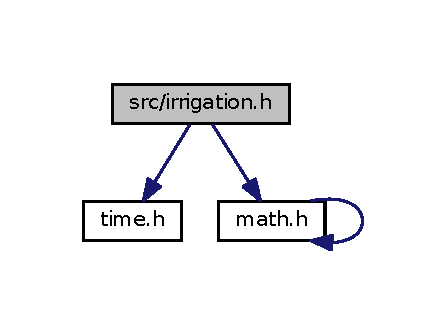
\includegraphics[width=214pt]{irrigation_8h__incl}
\end{center}
\end{figure}
This graph shows which files directly or indirectly include this file\+:\nopagebreak
\begin{figure}[H]
\begin{center}
\leavevmode
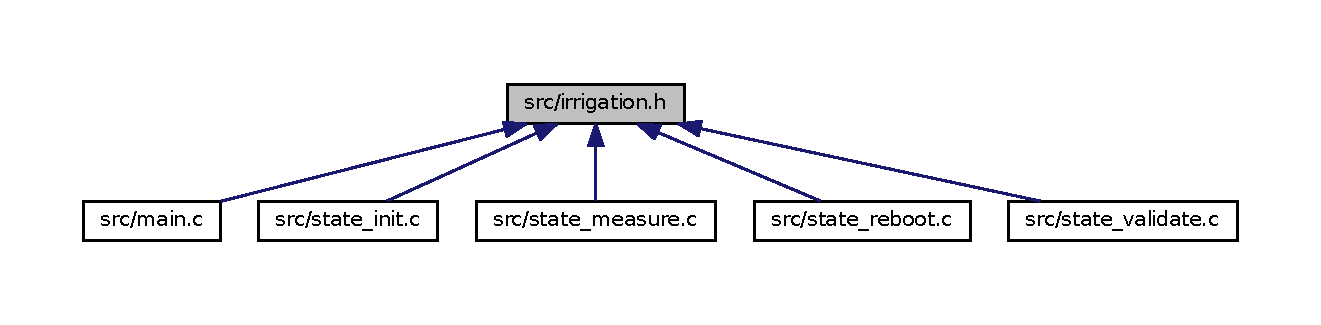
\includegraphics[width=350pt]{irrigation_8h__dep__incl}
\end{center}
\end{figure}
\subsection*{Classes}
\begin{DoxyCompactItemize}
\item 
struct \hyperlink{structirrigation__temperature__sample}{irrigation\+\_\+temperature\+\_\+sample}
\begin{DoxyCompactList}\small\item\em This is a timestamped temperature sample. \end{DoxyCompactList}\item 
struct \hyperlink{structirrigation__controller__status}{irrigation\+\_\+controller\+\_\+status}
\item 
struct \hyperlink{structirrigation__events}{irrigation\+\_\+events}
\begin{DoxyCompactList}\small\item\em The event callback functions for the irrigation controller core. \end{DoxyCompactList}\item 
struct \hyperlink{structirrigation__controller}{irrigation\+\_\+controller}
\begin{DoxyCompactList}\small\item\em Holds everything related to the irrigation controller. \end{DoxyCompactList}\end{DoxyCompactItemize}
\subsection*{Macros}
\begin{DoxyCompactItemize}
\item 
\#define \hyperlink{irrigation_8h_a98a17dc46f65ba67eb9c004ea48a9c2d}{time\+\_\+delta}(a,  b)~((float)(a.\+epoch -\/ b.\+epoch) + (float)(a.\+ms -\/ b.\+ms) / 1000.\+0)
\begin{DoxyCompactList}\small\item\em Calculates the time difference in seconds between two timestamps. \end{DoxyCompactList}\item 
\hypertarget{irrigation_8h_a8bb330be5fe982be9c1c28e70515043d}{}\#define {\bfseries \+\_\+\+I\+R\+R\+I\+G\+A\+T\+I\+O\+N\+\_\+\+H\+\_\+}\label{irrigation_8h_a8bb330be5fe982be9c1c28e70515043d}

\end{DoxyCompactItemize}
\subsection*{Enumerations}
\begin{DoxyCompactItemize}
\item 
enum \hyperlink{irrigation_8h_ac40bd72ec6942e213e454ebcacc92dc7}{irrigation\+\_\+status} \{ \\*
\hyperlink{irrigation_8h_ac40bd72ec6942e213e454ebcacc92dc7a64e8c241885100a4c6ee0dde8c084093}{irrigation\+\_\+status\+\_\+\+R\+E\+B\+O\+O\+T} = -\/2, 
\hyperlink{irrigation_8h_ac40bd72ec6942e213e454ebcacc92dc7a3d4b9190b0804578e02247c8cee11d8c}{irrigation\+\_\+status\+\_\+\+U\+N\+D\+E\+F\+I\+N\+E\+D} = -\/1, 
\hyperlink{irrigation_8h_ac40bd72ec6942e213e454ebcacc92dc7a0961e0972792be7ffcb4bf7aa64d4017}{irrigation\+\_\+status\+\_\+\+I\+N\+I\+T}, 
\hyperlink{irrigation_8h_ac40bd72ec6942e213e454ebcacc92dc7a0421b2d42223b25611688b6d2fe2d6e1}{irrigation\+\_\+status\+\_\+\+V\+A\+L\+I\+D\+A\+T\+E}, 
\\*
\hyperlink{irrigation_8h_ac40bd72ec6942e213e454ebcacc92dc7a1138583e9263588b98c16578bed06987}{irrigation\+\_\+status\+\_\+\+M\+E\+A\+S\+U\+R\+E}
 \}
\begin{DoxyCompactList}\small\item\em This is the state of the irrigation controller. \end{DoxyCompactList}\item 
enum \hyperlink{irrigation_8h_a9891f6b3b37611d2aebdb8601acdf6c6}{moisture\+\_\+sensor\+\_\+state} \{ \hyperlink{irrigation_8h_a9891f6b3b37611d2aebdb8601acdf6c6ad3f6b80b71bad74ea52dda2f31231cc3}{moisture\+\_\+sensor\+\_\+heating}, 
\hyperlink{irrigation_8h_a9891f6b3b37611d2aebdb8601acdf6c6a7e57547ef4980c1af315fd9937c976f0}{moisture\+\_\+sensor\+\_\+cooling}, 
\hyperlink{irrigation_8h_a9891f6b3b37611d2aebdb8601acdf6c6a4460d045ceb966a377b72d2825606fbd}{moisture\+\_\+sensor\+\_\+t1}, 
{\bfseries moisture\+\_\+sensor\+\_\+t2}
 \}
\begin{DoxyCompactList}\small\item\em This is the state of the moisture sensor. \end{DoxyCompactList}\end{DoxyCompactItemize}
\subsection*{Functions}
\begin{DoxyCompactItemize}
\item 
void \hyperlink{group__state__init_gaeca2f683660bf42f5258acd6aac353d0}{state\+\_\+init\+\_\+enter} (struct \hyperlink{structirrigation__controller}{irrigation\+\_\+controller} $\ast$controller)
\begin{DoxyCompactList}\small\item\em Reset all variables in the controller this state uses. \end{DoxyCompactList}\item 
void \hyperlink{group__state__init_ga5b5f5a7ec8534a643fb599efdee6ed4f}{state\+\_\+init\+\_\+run} (struct \hyperlink{structirrigation__controller}{irrigation\+\_\+controller} $\ast$controller)
\begin{DoxyCompactList}\small\item\em We will make a heart beat ramp for the status L\+E\+D while we wait for initial delay to complete. \end{DoxyCompactList}\item 
void \hyperlink{group__state__init_ga52863e306edb45d15c12acdecb7e5555}{state\+\_\+init\+\_\+exit} (struct \hyperlink{structirrigation__controller}{irrigation\+\_\+controller} $\ast$controller)
\begin{DoxyCompactList}\small\item\em Nothing has do be done before we leave this state. \end{DoxyCompactList}\item 
void \hyperlink{group__state__validate_gac0d41d4685bd461b3a613f6320405b79}{state\+\_\+validate\+\_\+enter} (struct \hyperlink{structirrigation__controller}{irrigation\+\_\+controller} $\ast$controller)
\begin{DoxyCompactList}\small\item\em We set up the validation timer and init the maximum and minim temperatured. \end{DoxyCompactList}\item 
void \hyperlink{group__state__validate_gaec38509b93f8a850919aa7a36e543ed5}{state\+\_\+validate\+\_\+run} (struct \hyperlink{structirrigation__controller}{irrigation\+\_\+controller} $\ast$controller)
\begin{DoxyCompactList}\small\item\em We have the heart beat L\+E\+D status and we update the minimum and maximum values while we continue to sample sensor data. \end{DoxyCompactList}\item 
void \hyperlink{group__state__validate_gac480e756742ffd9acd9bd21ac1e8885c}{state\+\_\+validate\+\_\+exit} (struct \hyperlink{structirrigation__controller}{irrigation\+\_\+controller} $\ast$controller)
\begin{DoxyCompactList}\small\item\em Nothing has to be done when we exit this state. \end{DoxyCompactList}\item 
\hypertarget{group__state__reboot_gab0e3409fa69ff96792cb5a768928a545}{}void {\bfseries state\+\_\+reboot\+\_\+enter} (struct \hyperlink{structirrigation__controller}{irrigation\+\_\+controller} $\ast$controller)\label{group__state__reboot_gab0e3409fa69ff96792cb5a768928a545}

\item 
\hypertarget{group__state__reboot_ga23cf1ecfb670c7c6c253a40705aa5caf}{}void {\bfseries state\+\_\+reboot\+\_\+run} (struct \hyperlink{structirrigation__controller}{irrigation\+\_\+controller} $\ast$controller)\label{group__state__reboot_ga23cf1ecfb670c7c6c253a40705aa5caf}

\item 
\hypertarget{group__state__reboot_gafbcdeb4b017f4350fb6ff51df410228b}{}void {\bfseries state\+\_\+reboot\+\_\+exit} (struct \hyperlink{structirrigation__controller}{irrigation\+\_\+controller} $\ast$controller)\label{group__state__reboot_gafbcdeb4b017f4350fb6ff51df410228b}

\item 
void \hyperlink{group__state__measure_ga24a42892ba25be220bff68fc151e0be7}{state\+\_\+measure\+\_\+enter} (struct \hyperlink{structirrigation__controller}{irrigation\+\_\+controller} $\ast$controller)
\begin{DoxyCompactList}\small\item\em Measure state enter. \end{DoxyCompactList}\item 
\hypertarget{group__state__measure_ga410776694bde81bde92a0b6b178ac015}{}void {\bfseries state\+\_\+measure\+\_\+run} (struct \hyperlink{structirrigation__controller}{irrigation\+\_\+controller} $\ast$controller)\label{group__state__measure_ga410776694bde81bde92a0b6b178ac015}

\item 
\hypertarget{group__state__measure_ga0f85f8645f5311e776e85a3697517266}{}void {\bfseries state\+\_\+measure\+\_\+exit} (struct \hyperlink{structirrigation__controller}{irrigation\+\_\+controller} $\ast$controller)\label{group__state__measure_ga0f85f8645f5311e776e85a3697517266}

\item 
\hypertarget{irrigation_8h_a6440cc6e50bc4445698e203198648185}{}void {\bfseries status\+\_\+color} (int r, int g, int b)\label{irrigation_8h_a6440cc6e50bc4445698e203198648185}

\end{DoxyCompactItemize}


\subsection{Detailed Description}
Irrigation main include file. 



\subsection{Macro Definition Documentation}
\hypertarget{irrigation_8h_a98a17dc46f65ba67eb9c004ea48a9c2d}{}\index{irrigation.\+h@{irrigation.\+h}!time\+\_\+delta@{time\+\_\+delta}}
\index{time\+\_\+delta@{time\+\_\+delta}!irrigation.\+h@{irrigation.\+h}}
\subsubsection[{time\+\_\+delta}]{\setlength{\rightskip}{0pt plus 5cm}\#define time\+\_\+delta(
\begin{DoxyParamCaption}
\item[{}]{a, }
\item[{}]{b}
\end{DoxyParamCaption}
)~((float)(a.\+epoch -\/ b.\+epoch) + (float)(a.\+ms -\/ b.\+ms) / 1000.\+0)}\label{irrigation_8h_a98a17dc46f65ba67eb9c004ea48a9c2d}


Calculates the time difference in seconds between two timestamps. 


\begin{DoxyParams}{Parameters}
{\em a} & Time event A \\
\hline
{\em b} & Time event B\\
\hline
\end{DoxyParams}
\begin{DoxyReturn}{Returns}
Returns a -\/ b 
\end{DoxyReturn}


Definition at line 11 of file irrigation.\+h.



Referenced by state\+\_\+measure\+\_\+enter(), state\+\_\+validate\+\_\+enter(), and state\+\_\+validate\+\_\+run().



\subsection{Enumeration Type Documentation}
\hypertarget{irrigation_8h_ac40bd72ec6942e213e454ebcacc92dc7}{}\index{irrigation.\+h@{irrigation.\+h}!irrigation\+\_\+status@{irrigation\+\_\+status}}
\index{irrigation\+\_\+status@{irrigation\+\_\+status}!irrigation.\+h@{irrigation.\+h}}
\subsubsection[{irrigation\+\_\+status}]{\setlength{\rightskip}{0pt plus 5cm}enum {\bf irrigation\+\_\+status}}\label{irrigation_8h_ac40bd72ec6942e213e454ebcacc92dc7}


This is the state of the irrigation controller. 

\begin{Desc}
\item[Enumerator]\par
\begin{description}
\index{irrigation\+\_\+status\+\_\+\+R\+E\+B\+O\+O\+T@{irrigation\+\_\+status\+\_\+\+R\+E\+B\+O\+O\+T}!irrigation.\+h@{irrigation.\+h}}\index{irrigation.\+h@{irrigation.\+h}!irrigation\+\_\+status\+\_\+\+R\+E\+B\+O\+O\+T@{irrigation\+\_\+status\+\_\+\+R\+E\+B\+O\+O\+T}}\item[{\em 
\hypertarget{irrigation_8h_ac40bd72ec6942e213e454ebcacc92dc7a64e8c241885100a4c6ee0dde8c084093}{}irrigation\+\_\+status\+\_\+\+R\+E\+B\+O\+O\+T\label{irrigation_8h_ac40bd72ec6942e213e454ebcacc92dc7a64e8c241885100a4c6ee0dde8c084093}
}]If something goes terribly wrong we can set this to pending state and force a reboot. \index{irrigation\+\_\+status\+\_\+\+U\+N\+D\+E\+F\+I\+N\+E\+D@{irrigation\+\_\+status\+\_\+\+U\+N\+D\+E\+F\+I\+N\+E\+D}!irrigation.\+h@{irrigation.\+h}}\index{irrigation.\+h@{irrigation.\+h}!irrigation\+\_\+status\+\_\+\+U\+N\+D\+E\+F\+I\+N\+E\+D@{irrigation\+\_\+status\+\_\+\+U\+N\+D\+E\+F\+I\+N\+E\+D}}\item[{\em 
\hypertarget{irrigation_8h_ac40bd72ec6942e213e454ebcacc92dc7a3d4b9190b0804578e02247c8cee11d8c}{}irrigation\+\_\+status\+\_\+\+U\+N\+D\+E\+F\+I\+N\+E\+D\label{irrigation_8h_ac40bd72ec6942e213e454ebcacc92dc7a3d4b9190b0804578e02247c8cee11d8c}
}]This is the default state but it is also used for the pending state when no pending state is set. \index{irrigation\+\_\+status\+\_\+\+I\+N\+I\+T@{irrigation\+\_\+status\+\_\+\+I\+N\+I\+T}!irrigation.\+h@{irrigation.\+h}}\index{irrigation.\+h@{irrigation.\+h}!irrigation\+\_\+status\+\_\+\+I\+N\+I\+T@{irrigation\+\_\+status\+\_\+\+I\+N\+I\+T}}\item[{\em 
\hypertarget{irrigation_8h_ac40bd72ec6942e213e454ebcacc92dc7a0961e0972792be7ffcb4bf7aa64d4017}{}irrigation\+\_\+status\+\_\+\+I\+N\+I\+T\label{irrigation_8h_ac40bd72ec6942e213e454ebcacc92dc7a0961e0972792be7ffcb4bf7aa64d4017}
}]Initialize the system. \index{irrigation\+\_\+status\+\_\+\+V\+A\+L\+I\+D\+A\+T\+E@{irrigation\+\_\+status\+\_\+\+V\+A\+L\+I\+D\+A\+T\+E}!irrigation.\+h@{irrigation.\+h}}\index{irrigation.\+h@{irrigation.\+h}!irrigation\+\_\+status\+\_\+\+V\+A\+L\+I\+D\+A\+T\+E@{irrigation\+\_\+status\+\_\+\+V\+A\+L\+I\+D\+A\+T\+E}}\item[{\em 
\hypertarget{irrigation_8h_ac40bd72ec6942e213e454ebcacc92dc7a0421b2d42223b25611688b6d2fe2d6e1}{}irrigation\+\_\+status\+\_\+\+V\+A\+L\+I\+D\+A\+T\+E\label{irrigation_8h_ac40bd72ec6942e213e454ebcacc92dc7a0421b2d42223b25611688b6d2fe2d6e1}
}]Validate the sensors. \index{irrigation\+\_\+status\+\_\+\+M\+E\+A\+S\+U\+R\+E@{irrigation\+\_\+status\+\_\+\+M\+E\+A\+S\+U\+R\+E}!irrigation.\+h@{irrigation.\+h}}\index{irrigation.\+h@{irrigation.\+h}!irrigation\+\_\+status\+\_\+\+M\+E\+A\+S\+U\+R\+E@{irrigation\+\_\+status\+\_\+\+M\+E\+A\+S\+U\+R\+E}}\item[{\em 
\hypertarget{irrigation_8h_ac40bd72ec6942e213e454ebcacc92dc7a1138583e9263588b98c16578bed06987}{}irrigation\+\_\+status\+\_\+\+M\+E\+A\+S\+U\+R\+E\label{irrigation_8h_ac40bd72ec6942e213e454ebcacc92dc7a1138583e9263588b98c16578bed06987}
}]Measure soil water content. \end{description}
\end{Desc}


Definition at line 23 of file irrigation.\+h.

\hypertarget{irrigation_8h_a9891f6b3b37611d2aebdb8601acdf6c6}{}\index{irrigation.\+h@{irrigation.\+h}!moisture\+\_\+sensor\+\_\+state@{moisture\+\_\+sensor\+\_\+state}}
\index{moisture\+\_\+sensor\+\_\+state@{moisture\+\_\+sensor\+\_\+state}!irrigation.\+h@{irrigation.\+h}}
\subsubsection[{moisture\+\_\+sensor\+\_\+state}]{\setlength{\rightskip}{0pt plus 5cm}enum {\bf moisture\+\_\+sensor\+\_\+state}}\label{irrigation_8h_a9891f6b3b37611d2aebdb8601acdf6c6}


This is the state of the moisture sensor. 

\begin{Desc}
\item[Enumerator]\par
\begin{description}
\index{moisture\+\_\+sensor\+\_\+heating@{moisture\+\_\+sensor\+\_\+heating}!irrigation.\+h@{irrigation.\+h}}\index{irrigation.\+h@{irrigation.\+h}!moisture\+\_\+sensor\+\_\+heating@{moisture\+\_\+sensor\+\_\+heating}}\item[{\em 
\hypertarget{irrigation_8h_a9891f6b3b37611d2aebdb8601acdf6c6ad3f6b80b71bad74ea52dda2f31231cc3}{}moisture\+\_\+sensor\+\_\+heating\label{irrigation_8h_a9891f6b3b37611d2aebdb8601acdf6c6ad3f6b80b71bad74ea52dda2f31231cc3}
}]The sensor is heating up. \index{moisture\+\_\+sensor\+\_\+cooling@{moisture\+\_\+sensor\+\_\+cooling}!irrigation.\+h@{irrigation.\+h}}\index{irrigation.\+h@{irrigation.\+h}!moisture\+\_\+sensor\+\_\+cooling@{moisture\+\_\+sensor\+\_\+cooling}}\item[{\em 
\hypertarget{irrigation_8h_a9891f6b3b37611d2aebdb8601acdf6c6a7e57547ef4980c1af315fd9937c976f0}{}moisture\+\_\+sensor\+\_\+cooling\label{irrigation_8h_a9891f6b3b37611d2aebdb8601acdf6c6a7e57547ef4980c1af315fd9937c976f0}
}]The sensor is cooling down. \index{moisture\+\_\+sensor\+\_\+t1@{moisture\+\_\+sensor\+\_\+t1}!irrigation.\+h@{irrigation.\+h}}\index{irrigation.\+h@{irrigation.\+h}!moisture\+\_\+sensor\+\_\+t1@{moisture\+\_\+sensor\+\_\+t1}}\item[{\em 
\hypertarget{irrigation_8h_a9891f6b3b37611d2aebdb8601acdf6c6a4460d045ceb966a377b72d2825606fbd}{}moisture\+\_\+sensor\+\_\+t1\label{irrigation_8h_a9891f6b3b37611d2aebdb8601acdf6c6a4460d045ceb966a377b72d2825606fbd}
}]\begin{DoxyRefDesc}{Todo}
\item[\hyperlink{todo__todo000003}{Todo}]t1 and t2 are not used for the moment \end{DoxyRefDesc}
\end{description}
\end{Desc}


Definition at line 40 of file irrigation.\+h.


\hypertarget{led__macro_8h}{}\section{src/led\+\_\+macro.h File Reference}
\label{led__macro_8h}\index{src/led\+\_\+macro.\+h@{src/led\+\_\+macro.\+h}}


Helper macros for L\+E\+D control.  


This graph shows which files directly or indirectly include this file\+:\nopagebreak
\begin{figure}[H]
\begin{center}
\leavevmode
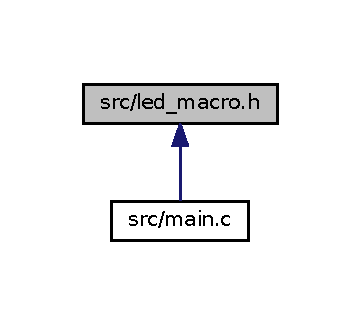
\includegraphics[width=173pt]{led__macro_8h__dep__incl}
\end{center}
\end{figure}
\subsection*{Macros}
\begin{DoxyCompactItemize}
\item 
\#define \hyperlink{led__macro_8h_a1a76ac28a3d1519a0aeac1be51a898a9}{G\+A\+M\+M\+A\+\_\+\+L\+U\+T\+\_\+8\+\_\+8\+\_\+\+E\+\_\+\+I\+N\+S\+T\+A\+N\+C\+E}(name)~const uint8\+\_\+t name\mbox{[}256\mbox{]} = \{0x0, 0x0, 0x0, 0x0, 0x0, 0x0, 0x0, 0x0, 0x0, 0x0, 0x0, 0x0, 0x0, 0x0, 0x0, 0x0, 0x0, 0x0, 0x0, 0x0, 0x0, 0x0, 0x0, 0x0, 0x0, 0x0, 0x0, 0x0, 0x0, 0x0, 0x0, 0x0, 0x0, 0x0, 0x1, 0x1, 0x1, 0x1, 0x1, 0x1, 0x1, 0x1, 0x1, 0x2, 0x2, 0x2, 0x2, 0x2, 0x2, 0x2, 0x3, 0x3, 0x3, 0x3, 0x3, 0x3, 0x4, 0x4, 0x4, 0x4, 0x4, 0x5, 0x5, 0x5, 0x5, 0x6, 0x6, 0x6, 0x7, 0x7, 0x7, 0x7, 0x8, 0x8, 0x8, 0x9, 0x9, 0x9, 0xa, 0xa, 0xa, 0xb, 0xb, 0xc, 0xc, 0xc, 0xd, 0xd, 0xe, 0xe, 0xf, 0xf, 0xf, 0x10, 0x10, 0x11, 0x11, 0x12, 0x12, 0x13, 0x14, 0x14, 0x15, 0x15, 0x16, 0x16, 0x17, 0x18, 0x18, 0x19, 0x19, 0x1a, 0x1b, 0x1b, 0x1c, 0x1d, 0x1d, 0x1e, 0x1f, 0x20, 0x20, 0x21, 0x22, 0x23, 0x23, 0x24, 0x25, 0x26, 0x27, 0x28, 0x28, 0x29, 0x2a, 0x2b, 0x2c, 0x2d, 0x2e, 0x2f, 0x30, 0x31, 0x31, 0x32, 0x33, 0x34, 0x35, 0x36, 0x38, 0x39, 0x3a, 0x3b, 0x3c, 0x3d, 0x3e, 0x3f, 0x40, 0x41, 0x43, 0x44, 0x45, 0x46, 0x47, 0x49, 0x4a, 0x4b, 0x4c, 0x4e, 0x4f, 0x50, 0x52, 0x53, 0x54, 0x56, 0x57, 0x58, 0x5a, 0x5b, 0x5d, 0x5e, 0x5f, 0x61, 0x62, 0x64, 0x65, 0x67, 0x69, 0x6a, 0x6c, 0x6d, 0x6f, 0x70, 0x72, 0x74, 0x75, 0x77, 0x79, 0x7a, 0x7c, 0x7e, 0x80, 0x81, 0x83, 0x85, 0x87, 0x89, 0x8b, 0x8c, 0x8e, 0x90, 0x92, 0x94, 0x96, 0x98, 0x9a, 0x9c, 0x9e, 0xa0, 0xa2, 0xa4, 0xa6, 0xa8, 0xaa, 0xac, 0xae, 0xb1, 0xb3, 0xb5, 0xb7, 0xb9, 0xbc, 0xbe, 0xc0, 0xc2, 0xc5, 0xc7, 0xc9, 0xcc, 0xce, 0xd0, 0xd3, 0xd5, 0xd8, 0xda, 0xdd, 0xdf, 0xe2, 0xe4, 0xe7, 0xe9, 0xec, 0xef, 0xf1, 0xf4, 0xf6, 0xf9, 0xfc, 0xff\}
\begin{DoxyCompactList}\small\item\em A gamma lookup table for 8 x 8 bits, exponent is mathematical constant e. \end{DoxyCompactList}\item 
\hypertarget{led__macro_8h_ae39da7dbcd8cae6896b83654dd6872e8}{}\#define {\bfseries \+\_\+\+L\+E\+D\+\_\+\+M\+A\+C\+R\+O\+\_\+\+H\+\_\+}\label{led__macro_8h_ae39da7dbcd8cae6896b83654dd6872e8}

\end{DoxyCompactItemize}


\subsection{Detailed Description}
Helper macros for L\+E\+D control. 



\subsection{Macro Definition Documentation}
\hypertarget{led__macro_8h_a1a76ac28a3d1519a0aeac1be51a898a9}{}\index{led\+\_\+macro.\+h@{led\+\_\+macro.\+h}!G\+A\+M\+M\+A\+\_\+\+L\+U\+T\+\_\+8\+\_\+8\+\_\+\+E\+\_\+\+I\+N\+S\+T\+A\+N\+C\+E@{G\+A\+M\+M\+A\+\_\+\+L\+U\+T\+\_\+8\+\_\+8\+\_\+\+E\+\_\+\+I\+N\+S\+T\+A\+N\+C\+E}}
\index{G\+A\+M\+M\+A\+\_\+\+L\+U\+T\+\_\+8\+\_\+8\+\_\+\+E\+\_\+\+I\+N\+S\+T\+A\+N\+C\+E@{G\+A\+M\+M\+A\+\_\+\+L\+U\+T\+\_\+8\+\_\+8\+\_\+\+E\+\_\+\+I\+N\+S\+T\+A\+N\+C\+E}!led\+\_\+macro.\+h@{led\+\_\+macro.\+h}}
\subsubsection[{G\+A\+M\+M\+A\+\_\+\+L\+U\+T\+\_\+8\+\_\+8\+\_\+\+E\+\_\+\+I\+N\+S\+T\+A\+N\+C\+E}]{\setlength{\rightskip}{0pt plus 5cm}\#define G\+A\+M\+M\+A\+\_\+\+L\+U\+T\+\_\+8\+\_\+8\+\_\+\+E\+\_\+\+I\+N\+S\+T\+A\+N\+C\+E(
\begin{DoxyParamCaption}
\item[{}]{name}
\end{DoxyParamCaption}
)~const uint8\+\_\+t name\mbox{[}256\mbox{]} = \{0x0, 0x0, 0x0, 0x0, 0x0, 0x0, 0x0, 0x0, 0x0, 0x0, 0x0, 0x0, 0x0, 0x0, 0x0, 0x0, 0x0, 0x0, 0x0, 0x0, 0x0, 0x0, 0x0, 0x0, 0x0, 0x0, 0x0, 0x0, 0x0, 0x0, 0x0, 0x0, 0x0, 0x0, 0x1, 0x1, 0x1, 0x1, 0x1, 0x1, 0x1, 0x1, 0x1, 0x2, 0x2, 0x2, 0x2, 0x2, 0x2, 0x2, 0x3, 0x3, 0x3, 0x3, 0x3, 0x3, 0x4, 0x4, 0x4, 0x4, 0x4, 0x5, 0x5, 0x5, 0x5, 0x6, 0x6, 0x6, 0x7, 0x7, 0x7, 0x7, 0x8, 0x8, 0x8, 0x9, 0x9, 0x9, 0xa, 0xa, 0xa, 0xb, 0xb, 0xc, 0xc, 0xc, 0xd, 0xd, 0xe, 0xe, 0xf, 0xf, 0xf, 0x10, 0x10, 0x11, 0x11, 0x12, 0x12, 0x13, 0x14, 0x14, 0x15, 0x15, 0x16, 0x16, 0x17, 0x18, 0x18, 0x19, 0x19, 0x1a, 0x1b, 0x1b, 0x1c, 0x1d, 0x1d, 0x1e, 0x1f, 0x20, 0x20, 0x21, 0x22, 0x23, 0x23, 0x24, 0x25, 0x26, 0x27, 0x28, 0x28, 0x29, 0x2a, 0x2b, 0x2c, 0x2d, 0x2e, 0x2f, 0x30, 0x31, 0x31, 0x32, 0x33, 0x34, 0x35, 0x36, 0x38, 0x39, 0x3a, 0x3b, 0x3c, 0x3d, 0x3e, 0x3f, 0x40, 0x41, 0x43, 0x44, 0x45, 0x46, 0x47, 0x49, 0x4a, 0x4b, 0x4c, 0x4e, 0x4f, 0x50, 0x52, 0x53, 0x54, 0x56, 0x57, 0x58, 0x5a, 0x5b, 0x5d, 0x5e, 0x5f, 0x61, 0x62, 0x64, 0x65, 0x67, 0x69, 0x6a, 0x6c, 0x6d, 0x6f, 0x70, 0x72, 0x74, 0x75, 0x77, 0x79, 0x7a, 0x7c, 0x7e, 0x80, 0x81, 0x83, 0x85, 0x87, 0x89, 0x8b, 0x8c, 0x8e, 0x90, 0x92, 0x94, 0x96, 0x98, 0x9a, 0x9c, 0x9e, 0xa0, 0xa2, 0xa4, 0xa6, 0xa8, 0xaa, 0xac, 0xae, 0xb1, 0xb3, 0xb5, 0xb7, 0xb9, 0xbc, 0xbe, 0xc0, 0xc2, 0xc5, 0xc7, 0xc9, 0xcc, 0xce, 0xd0, 0xd3, 0xd5, 0xd8, 0xda, 0xdd, 0xdf, 0xe2, 0xe4, 0xe7, 0xe9, 0xec, 0xef, 0xf1, 0xf4, 0xf6, 0xf9, 0xfc, 0xff\}}\label{led__macro_8h_a1a76ac28a3d1519a0aeac1be51a898a9}


A gamma lookup table for 8 x 8 bits, exponent is mathematical constant e. 



Definition at line 8 of file led\+\_\+macro.\+h.


\hypertarget{main_8c}{}\section{src/main.c File Reference}
\label{main_8c}\index{src/main.\+c@{src/main.\+c}}


Irrigation controller main file.  


{\ttfamily \#include \char`\"{}math.\+h\char`\"{}}\\*
{\ttfamily \#include \char`\"{}ws2812\+\_\+macro.\+h\char`\"{}}\\*
{\ttfamily \#include \char`\"{}usart\+\_\+macro.\+h\char`\"{}}\\*
{\ttfamily \#include \char`\"{}dma\+\_\+macro.\+h\char`\"{}}\\*
{\ttfamily \#include \char`\"{}led\+\_\+macro.\+h\char`\"{}}\\*
{\ttfamily \#include \char`\"{}timer\+\_\+macro.\+h\char`\"{}}\\*
{\ttfamily \#include \char`\"{}systick\+\_\+macro.\+h\char`\"{}}\\*
{\ttfamily \#include \char`\"{}adc.\+h\char`\"{}}\\*
{\ttfamily \#include \char`\"{}time.\+h\char`\"{}}\\*
{\ttfamily \#include \char`\"{}filter.\+h\char`\"{}}\\*
{\ttfamily \#include \char`\"{}irrigation.\+h\char`\"{}}\\*
Include dependency graph for main.\+c\+:
\nopagebreak
\begin{figure}[H]
\begin{center}
\leavevmode
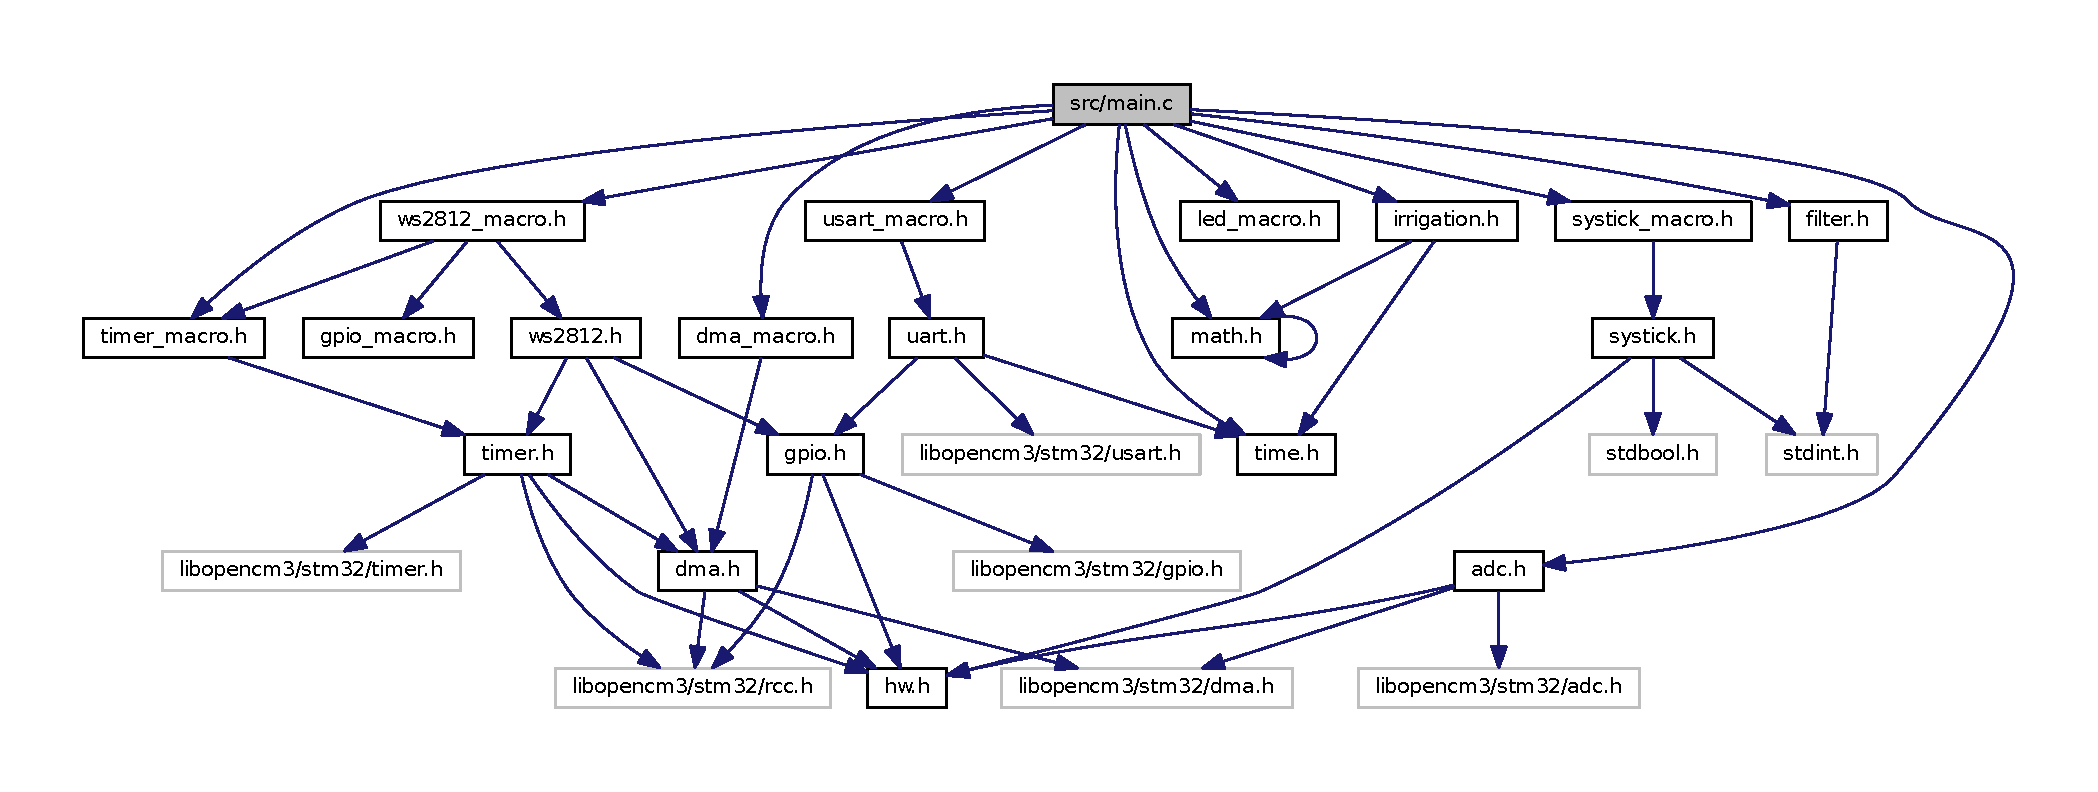
\includegraphics[width=350pt]{main_8c__incl}
\end{center}
\end{figure}
\subsection*{Macros}
\begin{DoxyCompactItemize}
\item 
\#define {\bfseries H\+W\+\_\+\+P\+R\+E\+\_\+\+I\+N\+I\+T}(call,  obj)
\end{DoxyCompactItemize}
\subsection*{Functions}
\begin{DoxyCompactItemize}
\item 
\hypertarget{main_8c_aa423cbe2bea57704cca655826b2338c1}{}{\bfseries G\+P\+I\+O\+\_\+\+P\+O\+R\+T\+\_\+\+I\+N\+S\+T\+A\+N\+C\+E} (G\+P\+I\+O\+\_\+\+P\+A, G\+P\+I\+O\+A, R\+C\+C\+\_\+\+G\+P\+I\+O\+A)\label{main_8c_aa423cbe2bea57704cca655826b2338c1}

\item 
\hypertarget{main_8c_abebbe5a8f2ebcfc52329af1a2a452c32}{}{\bfseries G\+P\+I\+O\+\_\+\+P\+O\+R\+T\+\_\+\+I\+N\+S\+T\+A\+N\+C\+E} (G\+P\+I\+O\+\_\+\+P\+B, G\+P\+I\+O\+B, R\+C\+C\+\_\+\+G\+P\+I\+O\+B)\label{main_8c_abebbe5a8f2ebcfc52329af1a2a452c32}

\item 
\hypertarget{main_8c_af239d1be6128c2cf9470dddd0736206d}{}{\bfseries G\+P\+I\+O\+\_\+\+P\+I\+N\+\_\+\+N\+O\+C\+O\+N\+F} (Serial\+\_\+tx,\&G\+P\+I\+O\+\_\+\+P\+A, G\+P\+I\+O\+\_\+\+U\+S\+A\+R\+T1\+\_\+\+T\+X)\label{main_8c_af239d1be6128c2cf9470dddd0736206d}

\item 
\hypertarget{main_8c_a4e07380dc740e8c8320b9ecf6fc1bd6d}{}{\bfseries U\+S\+A\+R\+T\+\_\+8\+N1} (Serial, U\+S\+A\+R\+T1, R\+C\+C\+\_\+\+U\+S\+A\+R\+T1, 921600, 0,\&Serial\+\_\+tx)\label{main_8c_a4e07380dc740e8c8320b9ecf6fc1bd6d}

\item 
\hypertarget{main_8c_ab6e1a812398e2960f55569f1becf22f8}{}{\bfseries D\+M\+A\+\_\+\+I\+N\+S\+T\+A\+N\+C\+E} (Dma, D\+M\+A1, R\+C\+C\+\_\+\+D\+M\+A1)\label{main_8c_ab6e1a812398e2960f55569f1becf22f8}

\item 
\hypertarget{main_8c_a2aeeaba0bf350894e16dca95c3433371}{}{\bfseries G\+P\+I\+O\+\_\+\+P\+I\+N\+\_\+\+N\+O\+C\+O\+N\+F} (Status\+L\+E\+D\+\_\+pin,\&G\+P\+I\+O\+\_\+\+P\+B, G\+P\+I\+O15)\label{main_8c_a2aeeaba0bf350894e16dca95c3433371}

\item 
\hypertarget{main_8c_a62bc4a3e73a3bda284d20e2d99aa9c3e}{}{\bfseries T\+I\+M\+E\+R\+\_\+\+N\+O\+C\+O\+N\+F} (Status\+L\+E\+D\+\_\+timer, T\+I\+M1, R\+C\+C\+\_\+\+T\+I\+M1)\label{main_8c_a62bc4a3e73a3bda284d20e2d99aa9c3e}

\item 
\hypertarget{main_8c_a65e33b62baadd843fc4d336930ffc80a}{}{\bfseries D\+M\+A\+\_\+\+C\+H\+A\+N\+N\+E\+L\+\_\+\+N\+O\+C\+O\+N\+F} (Status\+L\+E\+D\+\_\+dma,\&Dma, D\+M\+A\+\_\+\+C\+H\+A\+N\+N\+E\+L6)\label{main_8c_a65e33b62baadd843fc4d336930ffc80a}

\item 
\hypertarget{main_8c_a4b692da9c42d4defd8814f963d1d2da0}{}{\bfseries T\+I\+M\+E\+R\+\_\+\+C\+C\+R\+\_\+\+N\+O\+C\+O\+N\+F} (Status\+L\+E\+D\+\_\+pwm,\&Status\+L\+E\+D\+\_\+timer, T\+I\+M\+\_\+\+O\+C3\+N,\&Status\+L\+E\+D\+\_\+dma)\label{main_8c_a4b692da9c42d4defd8814f963d1d2da0}

\item 
\hypertarget{main_8c_ac01d8360f2847c41f234b2d6333879cc}{}{\bfseries S\+Y\+S\+T\+I\+C\+K\+\_\+\+A\+U\+T\+O\+\_\+\+C\+O\+N\+F\+I\+G} (Systick, 1000)\label{main_8c_ac01d8360f2847c41f234b2d6333879cc}

\item 
\hypertarget{main_8c_a1f98adee46907f4bd29dc153ce25dcb7}{}{\bfseries G\+A\+M\+M\+A\+\_\+\+L\+U\+T\+\_\+8\+\_\+8\+\_\+\+E\+\_\+\+I\+N\+S\+T\+A\+N\+C\+E} (L\+E\+D\+\_\+\+Gamma)\label{main_8c_a1f98adee46907f4bd29dc153ce25dcb7}

\item 
void \hyperlink{main_8c_aabae29cd362c0001a2b417c9206cb330}{hw\+\_\+init\+\_\+state} (enum \hyperlink{hw_8h_a3c02952100e7d051b77cdf060ca0ba9b}{hw\+\_\+init\+\_\+state} state)
\begin{DoxyCompactList}\small\item\em This function prototype calls all perhipherals with the state as argument. \end{DoxyCompactList}\item 
\hypertarget{main_8c_afdd94f850b193691f1bfc60c724b542a}{}void {\bfseries sys\+\_\+tick\+\_\+handler} (void)\label{main_8c_afdd94f850b193691f1bfc60c724b542a}

\item 
\hypertarget{main_8c_a359616b69ef6be09a3cb5680893c25cb}{}void {\bfseries ms\+\_\+sleep} (int time)\label{main_8c_a359616b69ef6be09a3cb5680893c25cb}

\item 
\hypertarget{main_8c_a42ca7c9b89c22fcd9ec9aeed3e96b6c4}{}void {\bfseries get\+\_\+system\+\_\+time\+\_\+blocking} (struct \hyperlink{structsw__timer__system__time}{sw\+\_\+timer\+\_\+system\+\_\+time} $\ast$result)\label{main_8c_a42ca7c9b89c22fcd9ec9aeed3e96b6c4}

\item 
\hypertarget{main_8c_ac10cd1ff6b8d3726905397fc86b44bb1}{}void {\bfseries set\+\_\+status\+\_\+color} (int r, int g, int b)\label{main_8c_ac10cd1ff6b8d3726905397fc86b44bb1}

\item 
\hypertarget{main_8c_a840291bc02cba5474a4cb46a9b9566fe}{}int {\bfseries main} (void)\label{main_8c_a840291bc02cba5474a4cb46a9b9566fe}

\end{DoxyCompactItemize}
\subsection*{Variables}
\begin{DoxyCompactItemize}
\item 
struct \hyperlink{structws2812__config}{ws2812\+\_\+config} {\bfseries Status\+L\+E\+D\+\_\+config}
\item 
\hypertarget{main_8c_ab0455c70d0edcf1a2a1c9ffc77fe5bee}{}struct \hyperlink{structws2812__rgb}{ws2812\+\_\+rgb} {\bfseries Status\+L\+E\+D\+\_\+buf} \mbox{[}1\mbox{]}\label{main_8c_ab0455c70d0edcf1a2a1c9ffc77fe5bee}

\item 
\hypertarget{main_8c_ae7d46441394e3638418869dda13a2970}{}volatile uint8\+\_\+t {\bfseries Status\+L\+E\+D\+\_\+pwmbuf} \mbox{[}1 $\ast$24+1\mbox{]}\label{main_8c_ae7d46441394e3638418869dda13a2970}

\item 
struct \hyperlink{structws2812}{ws2812} {\bfseries Status\+L\+E\+D}
\item 
\hypertarget{main_8c_ad6626ba12fbadd1981081605f892a7bb}{}volatile int {\bfseries sleep\+\_\+ms} = 0\label{main_8c_ad6626ba12fbadd1981081605f892a7bb}

\item 
\hypertarget{main_8c_a2d39b8e4f9506f28e2bdff70929287f6}{}volatile int {\bfseries N\+T\+C\+\_\+filtered\+\_\+value} = -\/1\label{main_8c_a2d39b8e4f9506f28e2bdff70929287f6}

\item 
\hypertarget{main_8c_a9d12c8106f421683f94175dd1c572624}{}volatile struct \hyperlink{structsw__timer__system__time}{sw\+\_\+timer\+\_\+system\+\_\+time} {\bfseries system\+\_\+time} = \{1420070400, 0\}\label{main_8c_a9d12c8106f421683f94175dd1c572624}

\item 
\hypertarget{main_8c_a153e3e14841d1967017a21ab4feacc19}{}volatile bool {\bfseries system\+\_\+time\+\_\+updated} =0\label{main_8c_a153e3e14841d1967017a21ab4feacc19}

\end{DoxyCompactItemize}


\subsection{Detailed Description}
Irrigation controller main file. 

\begin{DoxyRefDesc}{Todo}
\item[\hyperlink{todo__todo000005}{Todo}]systick, adc, moisture sensor, pwm output, filter 

explain port and rcc better\end{DoxyRefDesc}


\subsection{Macro Definition Documentation}
\hypertarget{main_8c_a3c3fdab7e413cd726f82bfba92630a39}{}\index{main.\+c@{main.\+c}!H\+W\+\_\+\+P\+R\+E\+\_\+\+I\+N\+I\+T@{H\+W\+\_\+\+P\+R\+E\+\_\+\+I\+N\+I\+T}}
\index{H\+W\+\_\+\+P\+R\+E\+\_\+\+I\+N\+I\+T@{H\+W\+\_\+\+P\+R\+E\+\_\+\+I\+N\+I\+T}!main.\+c@{main.\+c}}
\subsubsection[{H\+W\+\_\+\+P\+R\+E\+\_\+\+I\+N\+I\+T}]{\setlength{\rightskip}{0pt plus 5cm}\#define H\+W\+\_\+\+P\+R\+E\+\_\+\+I\+N\+I\+T(
\begin{DoxyParamCaption}
\item[{}]{call, }
\item[{}]{obj}
\end{DoxyParamCaption}
)}\label{main_8c_a3c3fdab7e413cd726f82bfba92630a39}
{\bfseries Value\+:}
\begin{DoxyCode}
call(obj, \hyperlink{hw_8h_a3c02952100e7d051b77cdf060ca0ba9baca0b4dbf0e3911b3edde56d700f76ecf}{HW\_INIT\_RCC});\(\backslash\)
    call(obj, \hyperlink{hw_8h_a3c02952100e7d051b77cdf060ca0ba9ba4e9b2d4b7e946d95c2e41f3de17035a0}{HW\_INIT\_GPIO});\(\backslash\)
    call(obj, \hyperlink{hw_8h_a3c02952100e7d051b77cdf060ca0ba9ba45012c00c17031e71a4f60ada04df07d}{HW\_INIT\_PRE\_NVIC});\(\backslash\)
    call(obj, \hyperlink{hw_8h_a3c02952100e7d051b77cdf060ca0ba9ba3f137ea5dd6b2ac372bb6d175434b3fa}{HW\_INIT\_NVIC});\(\backslash\)
    call(obj, \hyperlink{hw_8h_a3c02952100e7d051b77cdf060ca0ba9bacf9b04dc351d9fc47482fcd5229eb201}{HW\_INIT\_POST\_INIT});
\end{DoxyCode}


Definition at line 16 of file main.\+c.



\subsection{Function Documentation}
\hypertarget{main_8c_aabae29cd362c0001a2b417c9206cb330}{}\index{main.\+c@{main.\+c}!hw\+\_\+init\+\_\+state@{hw\+\_\+init\+\_\+state}}
\index{hw\+\_\+init\+\_\+state@{hw\+\_\+init\+\_\+state}!main.\+c@{main.\+c}}
\subsubsection[{hw\+\_\+init\+\_\+state}]{\setlength{\rightskip}{0pt plus 5cm}void {\bf hw\+\_\+init\+\_\+state} (
\begin{DoxyParamCaption}
\item[{enum {\bf hw\+\_\+init\+\_\+state}}]{state}
\end{DoxyParamCaption}
)}\label{main_8c_aabae29cd362c0001a2b417c9206cb330}


This function prototype calls all perhipherals with the state as argument. 



Definition at line 76 of file main.\+c.



References usart\+\_\+init(), and ws2812\+\_\+init().



\subsection{Variable Documentation}
\hypertarget{main_8c_a155a1d3f9591d851bbbe4d7d7ff71af7}{}\index{main.\+c@{main.\+c}!Status\+L\+E\+D@{Status\+L\+E\+D}}
\index{Status\+L\+E\+D@{Status\+L\+E\+D}!main.\+c@{main.\+c}}
\subsubsection[{Status\+L\+E\+D}]{\setlength{\rightskip}{0pt plus 5cm}struct {\bf ws2812} Status\+L\+E\+D}\label{main_8c_a155a1d3f9591d851bbbe4d7d7ff71af7}
{\bfseries Initial value\+:}
\begin{DoxyCode}
= \{
    .configuration = &StatusLED\_config,
    .led\_buffer = StatusLED\_buf,
    .pwm\_buffer = StatusLED\_pwmbuf,
    .led\_count = 1,
\}
\end{DoxyCode}


Definition at line 59 of file main.\+c.

\hypertarget{main_8c_aca1a1694194ca69da59aac0a1443da6e}{}\index{main.\+c@{main.\+c}!Status\+L\+E\+D\+\_\+config@{Status\+L\+E\+D\+\_\+config}}
\index{Status\+L\+E\+D\+\_\+config@{Status\+L\+E\+D\+\_\+config}!main.\+c@{main.\+c}}
\subsubsection[{Status\+L\+E\+D\+\_\+config}]{\setlength{\rightskip}{0pt plus 5cm}struct {\bf ws2812\+\_\+config} Status\+L\+E\+D\+\_\+config}\label{main_8c_aca1a1694194ca69da59aac0a1443da6e}
{\bfseries Initial value\+:}
\begin{DoxyCode}
= \{
    .ccr = &StatusLED\_pwm,
    .pin = &StatusLED\_pin,  
\}
\end{DoxyCode}


Definition at line 51 of file main.\+c.


\hypertarget{math_8h}{}\section{src/math.h File Reference}
\label{math_8h}\index{src/math.\+h@{src/math.\+h}}


Some math utilities.  


{\ttfamily \#include $<$math.\+h$>$}\\*
Include dependency graph for math.\+h\+:\nopagebreak
\begin{figure}[H]
\begin{center}
\leavevmode
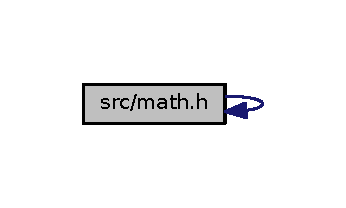
\includegraphics[width=166pt]{math_8h__incl}
\end{center}
\end{figure}
This graph shows which files directly or indirectly include this file\+:\nopagebreak
\begin{figure}[H]
\begin{center}
\leavevmode
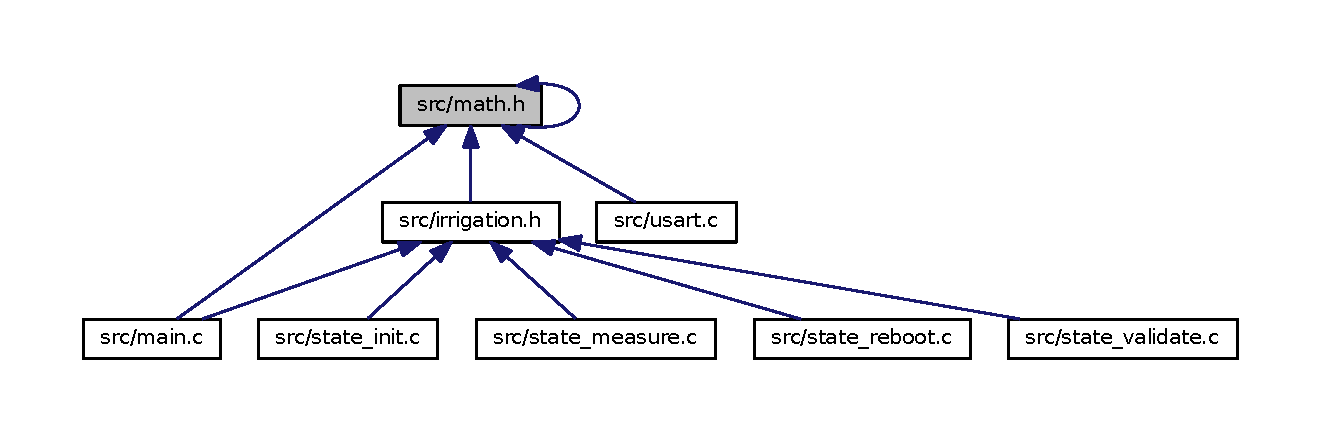
\includegraphics[width=350pt]{math_8h__dep__incl}
\end{center}
\end{figure}
\subsection*{Macros}
\begin{DoxyCompactItemize}
\item 
\#define \hyperlink{math_8h_a11511f39713c83a53bbf617c79d20cd6}{M\+A\+X}(v,  x)~((v $>$ x) ? v \+: x)
\begin{DoxyCompactList}\small\item\em Maximum of two scalars. \end{DoxyCompactList}\item 
\#define \hyperlink{math_8h_a267dc8ee2dc059cbd022d1c92ee86b4d}{M\+I\+N}(v,  x)~((v $<$ x) ? v \+: x)
\begin{DoxyCompactList}\small\item\em Minimum of two scalars. \end{DoxyCompactList}\item 
\#define \hyperlink{math_8h_ae438218ebea16c798a26d459bf3dd264}{math\+\_\+ramp}(var,  value)
\begin{DoxyCompactList}\small\item\em Triangle wave function with period 2.\+0. \end{DoxyCompactList}\item 
\hypertarget{math_8h_a2b382466fb3d64baed3a25a37fdd5beb}{}\#define {\bfseries \+\_\+\+M\+A\+T\+H\+\_\+\+H\+\_\+}\label{math_8h_a2b382466fb3d64baed3a25a37fdd5beb}

\end{DoxyCompactItemize}
\subsection*{Functions}
\begin{DoxyCompactItemize}
\item 
\hypertarget{math_8h_abc217116da1a947f370109db2274a714}{}unsigned long {\bfseries xorshf96} (void)\label{math_8h_abc217116da1a947f370109db2274a714}

\end{DoxyCompactItemize}


\subsection{Detailed Description}
Some math utilities. 



\subsection{Macro Definition Documentation}
\hypertarget{math_8h_ae438218ebea16c798a26d459bf3dd264}{}\index{math.\+h@{math.\+h}!math\+\_\+ramp@{math\+\_\+ramp}}
\index{math\+\_\+ramp@{math\+\_\+ramp}!math.\+h@{math.\+h}}
\subsubsection[{math\+\_\+ramp}]{\setlength{\rightskip}{0pt plus 5cm}\#define math\+\_\+ramp(
\begin{DoxyParamCaption}
\item[{}]{var, }
\item[{}]{value}
\end{DoxyParamCaption}
)}\label{math_8h_ae438218ebea16c798a26d459bf3dd264}
{\bfseries Value\+:}
\begin{DoxyCode}
\textcolor{keywordtype}{float} var = fmod(value, 2.0);\(\backslash\)
    if (var > 1) var = 2.0-var;
\end{DoxyCode}


Triangle wave function with period 2.\+0. 


\begin{DoxyParams}{Parameters}
{\em var} & Variable of result \\
\hline
{\em value} & Position in function \\
\hline
\end{DoxyParams}
\begin{DoxyReturn}{Returns}
float named var containing the function value 
\end{DoxyReturn}


Definition at line 24 of file math.\+h.



Referenced by state\+\_\+init\+\_\+run(), and state\+\_\+validate\+\_\+run().

\hypertarget{math_8h_a11511f39713c83a53bbf617c79d20cd6}{}\index{math.\+h@{math.\+h}!M\+A\+X@{M\+A\+X}}
\index{M\+A\+X@{M\+A\+X}!math.\+h@{math.\+h}}
\subsubsection[{M\+A\+X}]{\setlength{\rightskip}{0pt plus 5cm}\#define M\+A\+X(
\begin{DoxyParamCaption}
\item[{}]{v, }
\item[{}]{x}
\end{DoxyParamCaption}
)~((v $>$ x) ? v \+: x)}\label{math_8h_a11511f39713c83a53bbf617c79d20cd6}


Maximum of two scalars. 


\begin{DoxyParams}{Parameters}
{\em v} & First scalar \\
\hline
{\em x} & Second scalar \\
\hline
\end{DoxyParams}
\begin{DoxyReturn}{Returns}
The greates scalar 
\end{DoxyReturn}


Definition at line 12 of file math.\+h.



Referenced by state\+\_\+validate\+\_\+run().

\hypertarget{math_8h_a267dc8ee2dc059cbd022d1c92ee86b4d}{}\index{math.\+h@{math.\+h}!M\+I\+N@{M\+I\+N}}
\index{M\+I\+N@{M\+I\+N}!math.\+h@{math.\+h}}
\subsubsection[{M\+I\+N}]{\setlength{\rightskip}{0pt plus 5cm}\#define M\+I\+N(
\begin{DoxyParamCaption}
\item[{}]{v, }
\item[{}]{x}
\end{DoxyParamCaption}
)~((v $<$ x) ? v \+: x)}\label{math_8h_a267dc8ee2dc059cbd022d1c92ee86b4d}


Minimum of two scalars. 


\begin{DoxyParams}{Parameters}
{\em v} & First scalar \\
\hline
{\em x} & Second scalar \\
\hline
\end{DoxyParams}
\begin{DoxyReturn}{Returns}
The less scalar 
\end{DoxyReturn}


Definition at line 18 of file math.\+h.



Referenced by state\+\_\+validate\+\_\+run().


\hypertarget{state__init_8c}{}\section{src/state\+\_\+init.c File Reference}
\label{state__init_8c}\index{src/state\+\_\+init.\+c@{src/state\+\_\+init.\+c}}


Initial state.  


{\ttfamily \#include \char`\"{}irrigation.\+h\char`\"{}}\\*
Include dependency graph for state\+\_\+init.\+c\+:\nopagebreak
\begin{figure}[H]
\begin{center}
\leavevmode
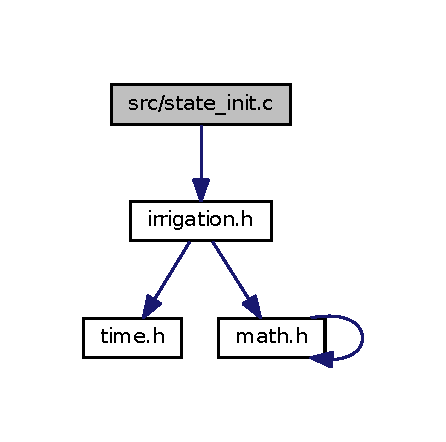
\includegraphics[width=214pt]{state__init_8c__incl}
\end{center}
\end{figure}
\subsection*{Functions}
\begin{DoxyCompactItemize}
\item 
void \hyperlink{group__state__init_gaeca2f683660bf42f5258acd6aac353d0}{state\+\_\+init\+\_\+enter} (struct \hyperlink{structirrigation__controller}{irrigation\+\_\+controller} $\ast$controller)
\begin{DoxyCompactList}\small\item\em Reset all variables in the controller this state uses. \end{DoxyCompactList}\item 
void \hyperlink{group__state__init_ga5b5f5a7ec8534a643fb599efdee6ed4f}{state\+\_\+init\+\_\+run} (struct \hyperlink{structirrigation__controller}{irrigation\+\_\+controller} $\ast$controller)
\begin{DoxyCompactList}\small\item\em We will make a heart beat ramp for the status L\+E\+D while we wait for initial delay to complete. \end{DoxyCompactList}\item 
void \hyperlink{group__state__init_ga52863e306edb45d15c12acdecb7e5555}{state\+\_\+init\+\_\+exit} (struct \hyperlink{structirrigation__controller}{irrigation\+\_\+controller} $\ast$controller)
\begin{DoxyCompactList}\small\item\em Nothing has do be done before we leave this state. \end{DoxyCompactList}\end{DoxyCompactItemize}


\subsection{Detailed Description}
Initial state. 


\hypertarget{state__measure_8c}{}\section{src/state\+\_\+measure.c File Reference}
\label{state__measure_8c}\index{src/state\+\_\+measure.\+c@{src/state\+\_\+measure.\+c}}


Measurement state.  


{\ttfamily \#include \char`\"{}irrigation.\+h\char`\"{}}\\*
Include dependency graph for state\+\_\+measure.\+c\+:\nopagebreak
\begin{figure}[H]
\begin{center}
\leavevmode
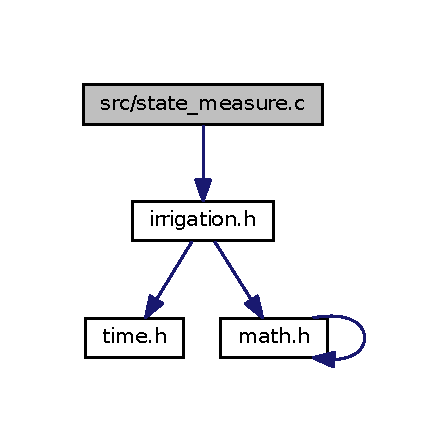
\includegraphics[width=215pt]{state__measure_8c__incl}
\end{center}
\end{figure}
\subsection*{Functions}
\begin{DoxyCompactItemize}
\item 
void \hyperlink{group__state__measure_ga24a42892ba25be220bff68fc151e0be7}{state\+\_\+measure\+\_\+enter} (struct \hyperlink{structirrigation__controller}{irrigation\+\_\+controller} $\ast$controller)
\begin{DoxyCompactList}\small\item\em Measure state enter. \end{DoxyCompactList}\item 
\hypertarget{group__state__measure_ga410776694bde81bde92a0b6b178ac015}{}void {\bfseries state\+\_\+measure\+\_\+run} (struct \hyperlink{structirrigation__controller}{irrigation\+\_\+controller} $\ast$controller)\label{group__state__measure_ga410776694bde81bde92a0b6b178ac015}

\item 
\hypertarget{group__state__measure_ga0f85f8645f5311e776e85a3697517266}{}void {\bfseries state\+\_\+measure\+\_\+exit} (struct \hyperlink{structirrigation__controller}{irrigation\+\_\+controller} $\ast$controller)\label{group__state__measure_ga0f85f8645f5311e776e85a3697517266}

\end{DoxyCompactItemize}


\subsection{Detailed Description}
Measurement state. 


\hypertarget{state__reboot_8c}{}\section{src/state\+\_\+reboot.c File Reference}
\label{state__reboot_8c}\index{src/state\+\_\+reboot.\+c@{src/state\+\_\+reboot.\+c}}


Rebooting state.  


{\ttfamily \#include \char`\"{}irrigation.\+h\char`\"{}}\\*
Include dependency graph for state\+\_\+reboot.\+c\+:\nopagebreak
\begin{figure}[H]
\begin{center}
\leavevmode
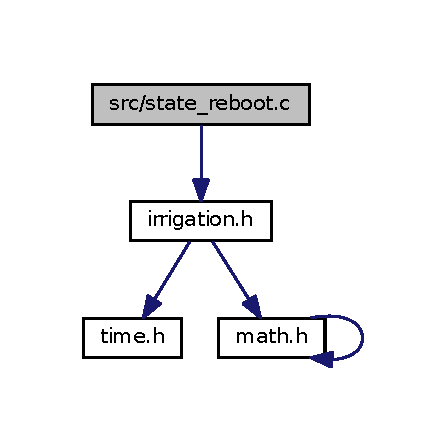
\includegraphics[width=214pt]{state__reboot_8c__incl}
\end{center}
\end{figure}
\subsection*{Functions}
\begin{DoxyCompactItemize}
\item 
\hypertarget{group__state__reboot_gab0e3409fa69ff96792cb5a768928a545}{}void {\bfseries state\+\_\+reboot\+\_\+enter} (struct \hyperlink{structirrigation__controller}{irrigation\+\_\+controller} $\ast$controller)\label{group__state__reboot_gab0e3409fa69ff96792cb5a768928a545}

\item 
\hypertarget{group__state__reboot_ga23cf1ecfb670c7c6c253a40705aa5caf}{}void {\bfseries state\+\_\+reboot\+\_\+run} (struct \hyperlink{structirrigation__controller}{irrigation\+\_\+controller} $\ast$controller)\label{group__state__reboot_ga23cf1ecfb670c7c6c253a40705aa5caf}

\item 
\hypertarget{group__state__reboot_gafbcdeb4b017f4350fb6ff51df410228b}{}void {\bfseries state\+\_\+reboot\+\_\+exit} (struct \hyperlink{structirrigation__controller}{irrigation\+\_\+controller} $\ast$controller)\label{group__state__reboot_gafbcdeb4b017f4350fb6ff51df410228b}

\end{DoxyCompactItemize}


\subsection{Detailed Description}
Rebooting state. 


\hypertarget{state__validate_8c}{}\section{src/state\+\_\+validate.c File Reference}
\label{state__validate_8c}\index{src/state\+\_\+validate.\+c@{src/state\+\_\+validate.\+c}}


Sensor validation state.  


{\ttfamily \#include \char`\"{}irrigation.\+h\char`\"{}}\\*
Include dependency graph for state\+\_\+validate.\+c\+:\nopagebreak
\begin{figure}[H]
\begin{center}
\leavevmode
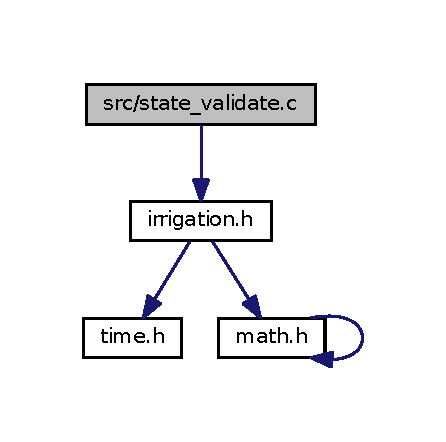
\includegraphics[width=214pt]{state__validate_8c__incl}
\end{center}
\end{figure}
\subsection*{Functions}
\begin{DoxyCompactItemize}
\item 
void \hyperlink{group__state__validate_gac0d41d4685bd461b3a613f6320405b79}{state\+\_\+validate\+\_\+enter} (struct \hyperlink{structirrigation__controller}{irrigation\+\_\+controller} $\ast$controller)
\begin{DoxyCompactList}\small\item\em We set up the validation timer and init the maximum and minim temperatured. \end{DoxyCompactList}\item 
void \hyperlink{group__state__validate_gaec38509b93f8a850919aa7a36e543ed5}{state\+\_\+validate\+\_\+run} (struct \hyperlink{structirrigation__controller}{irrigation\+\_\+controller} $\ast$controller)
\begin{DoxyCompactList}\small\item\em We have the heart beat L\+E\+D status and we update the minimum and maximum values while we continue to sample sensor data. \end{DoxyCompactList}\item 
void \hyperlink{group__state__validate_gac480e756742ffd9acd9bd21ac1e8885c}{state\+\_\+validate\+\_\+exit} (struct \hyperlink{structirrigation__controller}{irrigation\+\_\+controller} $\ast$controller)
\begin{DoxyCompactList}\small\item\em Nothing has to be done when we exit this state. \end{DoxyCompactList}\end{DoxyCompactItemize}


\subsection{Detailed Description}
Sensor validation state. 


\hypertarget{systick_8c}{}\section{src/systick.c File Reference}
\label{systick_8c}\index{src/systick.\+c@{src/systick.\+c}}


Systick H\+A\+L implementation.  


{\ttfamily \#include \char`\"{}systick.\+h\char`\"{}}\\*
{\ttfamily \#include $<$libopencm3/cm3/systick.\+h$>$}\\*
{\ttfamily \#include $<$libopencm3/stm32/rcc.\+h$>$}\\*
Include dependency graph for systick.\+c\+:\nopagebreak
\begin{figure}[H]
\begin{center}
\leavevmode
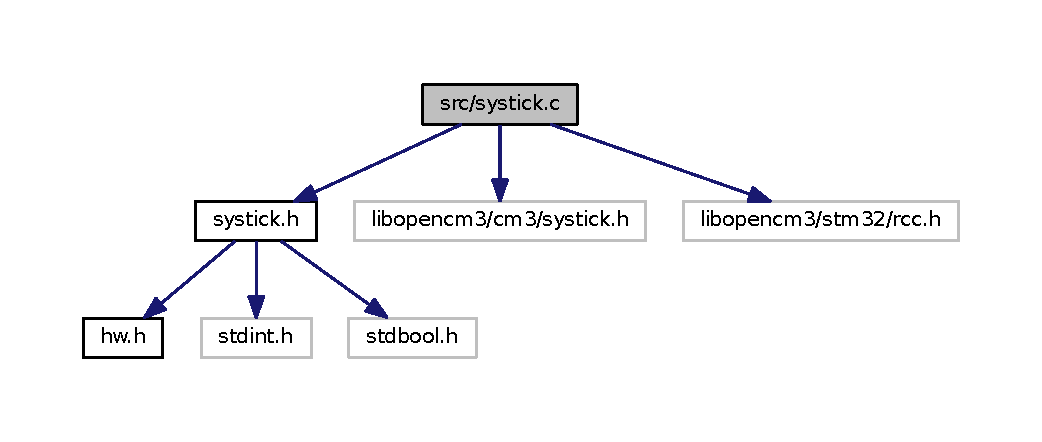
\includegraphics[width=350pt]{systick_8c__incl}
\end{center}
\end{figure}
\subsection*{Functions}
\begin{DoxyCompactItemize}
\item 
\hypertarget{systick_8c_a94410297949376c726ff1a24dc8d40c3}{}void {\bfseries systick\+\_\+init} (struct \hyperlink{structsystick}{systick} $\ast$\hyperlink{structsystick}{systick}, enum \hyperlink{hw_8h_a3c02952100e7d051b77cdf060ca0ba9b}{hw\+\_\+init\+\_\+state} state)\label{systick_8c_a94410297949376c726ff1a24dc8d40c3}

\end{DoxyCompactItemize}


\subsection{Detailed Description}
Systick H\+A\+L implementation. 


\hypertarget{systick_8h}{}\section{src/systick.h File Reference}
\label{systick_8h}\index{src/systick.\+h@{src/systick.\+h}}


systick H\+A\+L include  


{\ttfamily \#include \char`\"{}hw.\+h\char`\"{}}\\*
{\ttfamily \#include $<$stdint.\+h$>$}\\*
{\ttfamily \#include $<$stdbool.\+h$>$}\\*
Include dependency graph for systick.\+h\+:\nopagebreak
\begin{figure}[H]
\begin{center}
\leavevmode
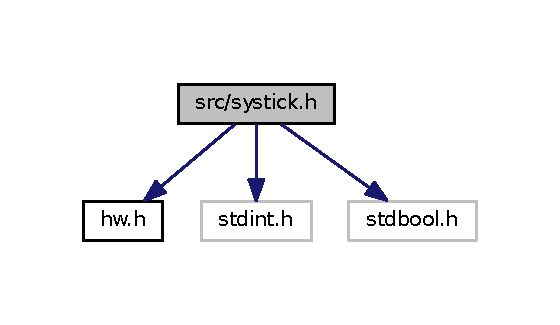
\includegraphics[width=269pt]{systick_8h__incl}
\end{center}
\end{figure}
This graph shows which files directly or indirectly include this file\+:
\nopagebreak
\begin{figure}[H]
\begin{center}
\leavevmode
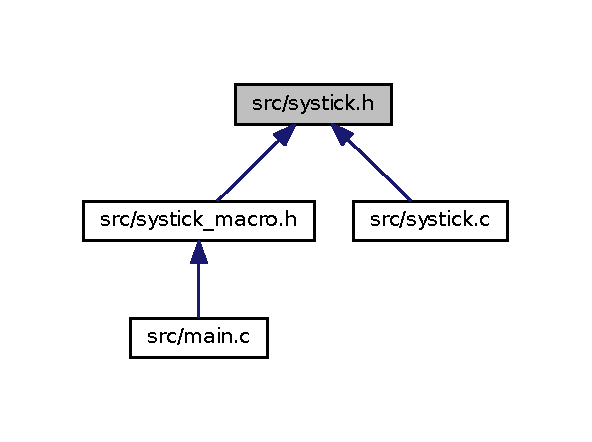
\includegraphics[width=284pt]{systick_8h__dep__incl}
\end{center}
\end{figure}
\subsection*{Classes}
\begin{DoxyCompactItemize}
\item 
struct \hyperlink{structsystick__config}{systick\+\_\+config}
\item 
struct \hyperlink{structsystick}{systick}
\end{DoxyCompactItemize}
\subsection*{Functions}
\begin{DoxyCompactItemize}
\item 
\hypertarget{systick_8h_a94410297949376c726ff1a24dc8d40c3}{}void {\bfseries systick\+\_\+init} (struct \hyperlink{structsystick}{systick} $\ast$\hyperlink{structsystick}{systick}, enum \hyperlink{hw_8h_a3c02952100e7d051b77cdf060ca0ba9b}{hw\+\_\+init\+\_\+state} state)\label{systick_8h_a94410297949376c726ff1a24dc8d40c3}

\end{DoxyCompactItemize}


\subsection{Detailed Description}
systick H\+A\+L include 


\hypertarget{time_8c}{}\section{src/time.c File Reference}
\label{time_8c}\index{src/time.\+c@{src/time.\+c}}


Time keeping and conversation functions.  


{\ttfamily \#include \char`\"{}time.\+h\char`\"{}}\\*
Include dependency graph for time.\+c\+:\nopagebreak
\begin{figure}[H]
\begin{center}
\leavevmode
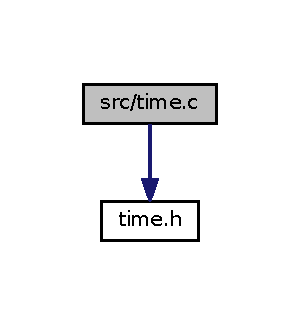
\includegraphics[width=144pt]{time_8c__incl}
\end{center}
\end{figure}
\subsection*{Macros}
\begin{DoxyCompactItemize}
\item 
\hypertarget{time_8c_af900e330dd6141d60b06a37630bbb086}{}\#define {\bfseries L\+E\+A\+P\+O\+C\+H}~(946684800\+L\+L + 86400$\ast$(31+29))\label{time_8c_af900e330dd6141d60b06a37630bbb086}

\item 
\hypertarget{time_8c_ad12582857140762bf2a39614d05f3a27}{}\#define {\bfseries D\+A\+Y\+S\+\_\+\+P\+E\+R\+\_\+400\+Y}~(365$\ast$400 + 97)\label{time_8c_ad12582857140762bf2a39614d05f3a27}

\item 
\hypertarget{time_8c_aa9dc1f7a73d6fd0a34361bc3cb85b91d}{}\#define {\bfseries D\+A\+Y\+S\+\_\+\+P\+E\+R\+\_\+100\+Y}~(365$\ast$100 + 24)\label{time_8c_aa9dc1f7a73d6fd0a34361bc3cb85b91d}

\item 
\hypertarget{time_8c_a46ad88cd30c4b5546d27510f09840340}{}\#define {\bfseries D\+A\+Y\+S\+\_\+\+P\+E\+R\+\_\+4\+Y}~(365$\ast$4   + 1)\label{time_8c_a46ad88cd30c4b5546d27510f09840340}

\end{DoxyCompactItemize}
\subsection*{Functions}
\begin{DoxyCompactItemize}
\item 
int \hyperlink{time_8c_a356fcdd74b8b159a7de9b87dcb694617}{time\+\_\+tm\+\_\+from\+\_\+epoch} (struct \hyperlink{structtm}{tm} $\ast$\hyperlink{structtm}{tm}, int t)
\begin{DoxyCompactList}\small\item\em Convert epoch time to struct tm. \end{DoxyCompactList}\end{DoxyCompactItemize}


\subsection{Detailed Description}
Time keeping and conversation functions. 



\subsection{Function Documentation}
\hypertarget{time_8c_a356fcdd74b8b159a7de9b87dcb694617}{}\index{time.\+c@{time.\+c}!time\+\_\+tm\+\_\+from\+\_\+epoch@{time\+\_\+tm\+\_\+from\+\_\+epoch}}
\index{time\+\_\+tm\+\_\+from\+\_\+epoch@{time\+\_\+tm\+\_\+from\+\_\+epoch}!time.\+c@{time.\+c}}
\subsubsection[{time\+\_\+tm\+\_\+from\+\_\+epoch}]{\setlength{\rightskip}{0pt plus 5cm}int time\+\_\+tm\+\_\+from\+\_\+epoch (
\begin{DoxyParamCaption}
\item[{struct {\bf tm} $\ast$}]{tm, }
\item[{int}]{t}
\end{DoxyParamCaption}
)}\label{time_8c_a356fcdd74b8b159a7de9b87dcb694617}


Convert epoch time to struct tm. 

Based on \href{http://git.musl-libc.org/cgit/musl/tree/src/time/__secs_to_tm.c}{\tt http\+://git.\+musl-\/libc.\+org/cgit/musl/tree/src/time/\+\_\+\+\_\+secs\+\_\+to\+\_\+tm.\+c}


\begin{DoxyParams}{Parameters}
{\em tm} & Pointer to target struct tm \\
\hline
{\em t} & Epoch time \\
\hline
\end{DoxyParams}
\begin{DoxyReturn}{Returns}
0 on success 
\end{DoxyReturn}


Definition at line 27 of file time.\+c.



References tm\+::tm\+\_\+hour, tm\+::tm\+\_\+mday, tm\+::tm\+\_\+min, tm\+::tm\+\_\+mon, tm\+::tm\+\_\+sec, tm\+::tm\+\_\+wday, tm\+::tm\+\_\+yday, and tm\+::tm\+\_\+year.



Referenced by usart\+\_\+blocking\+\_\+tm().


\hypertarget{time_8h}{}\section{src/time.h File Reference}
\label{time_8h}\index{src/time.\+h@{src/time.\+h}}


Time keeping and converting include file.  


This graph shows which files directly or indirectly include this file\+:
\nopagebreak
\begin{figure}[H]
\begin{center}
\leavevmode
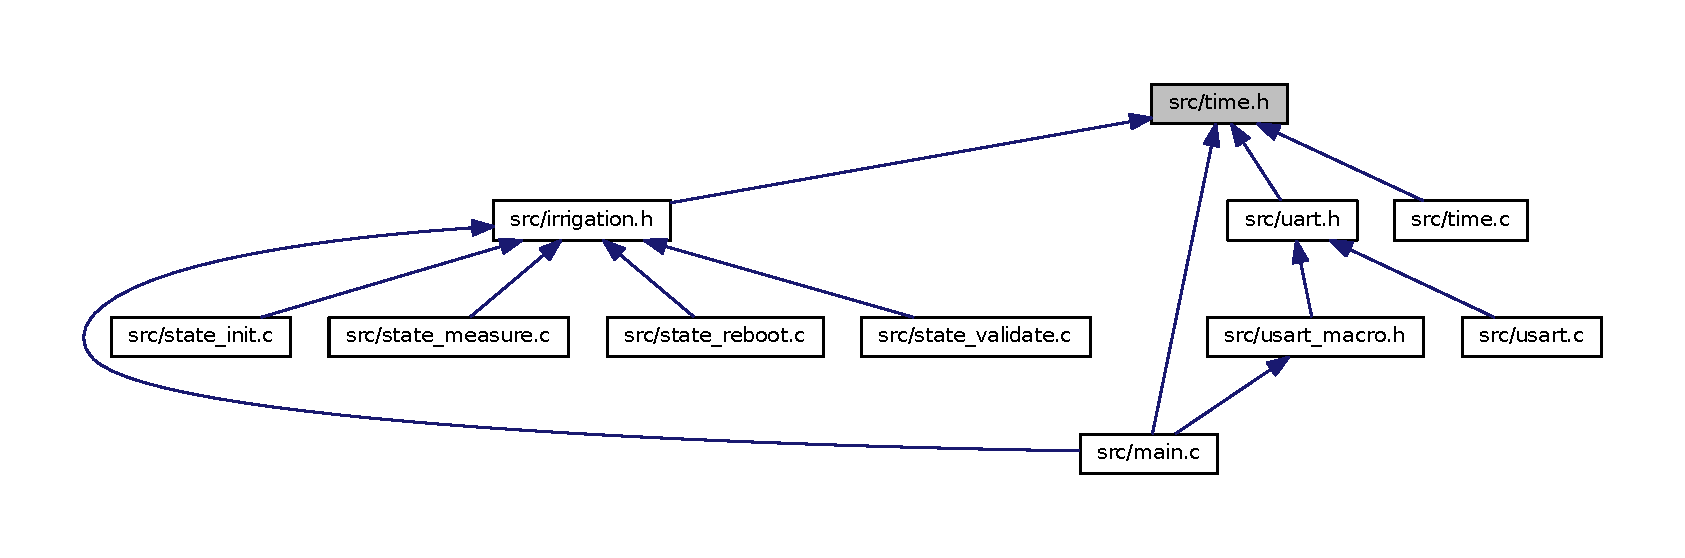
\includegraphics[width=350pt]{time_8h__dep__incl}
\end{center}
\end{figure}
\subsection*{Classes}
\begin{DoxyCompactItemize}
\item 
struct \hyperlink{structtm}{tm}
\begin{DoxyCompactList}\small\item\em Broken down time. \end{DoxyCompactList}\item 
struct \hyperlink{structsw__timer__system__time}{sw\+\_\+timer\+\_\+system\+\_\+time}
\begin{DoxyCompactList}\small\item\em Timestamp. \end{DoxyCompactList}\end{DoxyCompactItemize}
\subsection*{Functions}
\begin{DoxyCompactItemize}
\item 
int \hyperlink{time_8h_a5820d1723388d23f68df400cc4a6a065}{time\+\_\+tm\+\_\+from\+\_\+epoch} (struct \hyperlink{structtm}{tm} $\ast$result, int epoch)
\begin{DoxyCompactList}\small\item\em Convert epoch time to struct tm. \end{DoxyCompactList}\end{DoxyCompactItemize}


\subsection{Detailed Description}
Time keeping and converting include file. 



\subsection{Function Documentation}
\hypertarget{time_8h_a5820d1723388d23f68df400cc4a6a065}{}\index{time.\+h@{time.\+h}!time\+\_\+tm\+\_\+from\+\_\+epoch@{time\+\_\+tm\+\_\+from\+\_\+epoch}}
\index{time\+\_\+tm\+\_\+from\+\_\+epoch@{time\+\_\+tm\+\_\+from\+\_\+epoch}!time.\+h@{time.\+h}}
\subsubsection[{time\+\_\+tm\+\_\+from\+\_\+epoch}]{\setlength{\rightskip}{0pt plus 5cm}int time\+\_\+tm\+\_\+from\+\_\+epoch (
\begin{DoxyParamCaption}
\item[{struct {\bf tm} $\ast$}]{tm, }
\item[{int}]{t}
\end{DoxyParamCaption}
)}\label{time_8h_a5820d1723388d23f68df400cc4a6a065}


Convert epoch time to struct tm. 

Based on \href{http://git.musl-libc.org/cgit/musl/tree/src/time/__secs_to_tm.c}{\tt http\+://git.\+musl-\/libc.\+org/cgit/musl/tree/src/time/\+\_\+\+\_\+secs\+\_\+to\+\_\+tm.\+c}


\begin{DoxyParams}{Parameters}
{\em tm} & Pointer to target struct tm \\
\hline
{\em t} & Epoch time \\
\hline
\end{DoxyParams}
\begin{DoxyReturn}{Returns}
0 on success 
\end{DoxyReturn}


Definition at line 27 of file time.\+c.



References tm\+::tm\+\_\+hour, tm\+::tm\+\_\+mday, tm\+::tm\+\_\+min, tm\+::tm\+\_\+mon, tm\+::tm\+\_\+sec, tm\+::tm\+\_\+wday, tm\+::tm\+\_\+yday, and tm\+::tm\+\_\+year.



Referenced by usart\+\_\+blocking\+\_\+tm().


\hypertarget{timer_8c}{}\section{src/timer.c File Reference}
\label{timer_8c}\index{src/timer.\+c@{src/timer.\+c}}


Timer H\+A\+L implementation.  


{\ttfamily \#include \char`\"{}timer.\+h\char`\"{}}\\*
Include dependency graph for timer.\+c\+:\nopagebreak
\begin{figure}[H]
\begin{center}
\leavevmode
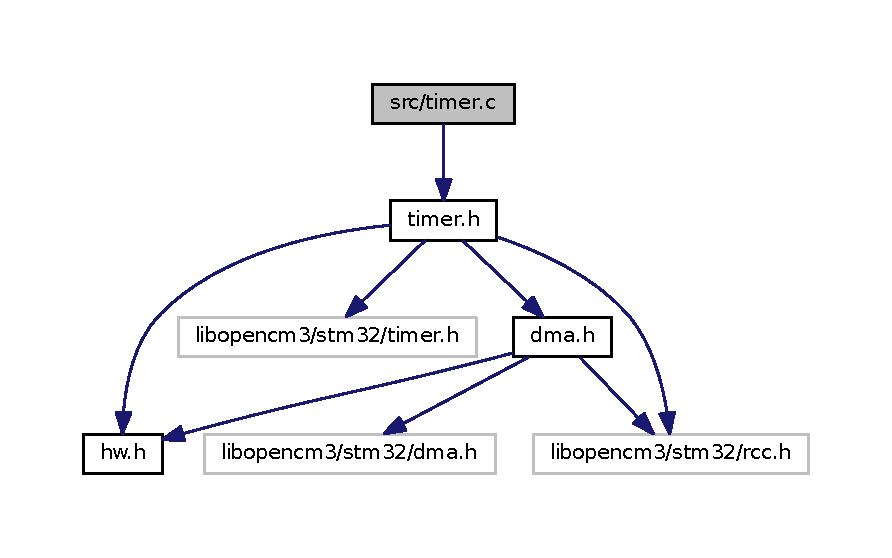
\includegraphics[width=350pt]{timer_8c__incl}
\end{center}
\end{figure}
\subsection*{Functions}
\begin{DoxyCompactItemize}
\item 
void \hyperlink{timer_8c_a995539ac62815c22bad2313f304865b5}{timer\+\_\+ccr\+\_\+init} (struct \hyperlink{structtimer__ccr}{timer\+\_\+ccr} $\ast$ccr, enum \hyperlink{hw_8h_a3c02952100e7d051b77cdf060ca0ba9b}{hw\+\_\+init\+\_\+state} state)
\begin{DoxyCompactList}\small\item\em Upgrade \hyperlink{structtimer__ccr}{timer\+\_\+ccr} state and init hardware. \end{DoxyCompactList}\item 
void \hyperlink{timer_8c_a734417848b07d1d04bca5e224f13e319}{timer\+\_\+ccr\+\_\+set} (struct \hyperlink{structtimer__ccr}{timer\+\_\+ccr} $\ast$ccr, uint32\+\_\+t value)
\begin{DoxyCompactList}\small\item\em Set C\+C\+R value of \hyperlink{structtimer__ccr}{timer\+\_\+ccr}. \end{DoxyCompactList}\item 
void \hyperlink{timer_8c_a1e33eb6cb5bd4bd99416edbb25790760}{timer\+\_\+init} (struct \hyperlink{structtimer}{timer} $\ast$\hyperlink{structtimer}{timer}, enum \hyperlink{hw_8h_a3c02952100e7d051b77cdf060ca0ba9b}{hw\+\_\+init\+\_\+state} state)
\begin{DoxyCompactList}\small\item\em Upgrade timer\+\_\+init state and init hardware. \end{DoxyCompactList}\end{DoxyCompactItemize}


\subsection{Detailed Description}
Timer H\+A\+L implementation. 



\subsection{Function Documentation}
\hypertarget{timer_8c_a995539ac62815c22bad2313f304865b5}{}\index{timer.\+c@{timer.\+c}!timer\+\_\+ccr\+\_\+init@{timer\+\_\+ccr\+\_\+init}}
\index{timer\+\_\+ccr\+\_\+init@{timer\+\_\+ccr\+\_\+init}!timer.\+c@{timer.\+c}}
\subsubsection[{timer\+\_\+ccr\+\_\+init}]{\setlength{\rightskip}{0pt plus 5cm}void timer\+\_\+ccr\+\_\+init (
\begin{DoxyParamCaption}
\item[{struct {\bf timer\+\_\+ccr} $\ast$}]{ccr, }
\item[{enum {\bf hw\+\_\+init\+\_\+state}}]{state}
\end{DoxyParamCaption}
)}\label{timer_8c_a995539ac62815c22bad2313f304865b5}


Upgrade \hyperlink{structtimer__ccr}{timer\+\_\+ccr} state and init hardware. 

\begin{DoxyRefDesc}{Todo}
\item[\hyperlink{todo__todo000006}{Todo}]Add more C\+C\+R-\/channels \end{DoxyRefDesc}


\begin{DoxyRefDesc}{Todo}
\item[\hyperlink{todo__todo000007}{Todo}]Only upgrade state if needed \end{DoxyRefDesc}


Definition at line 12 of file timer.\+c.



References D\+E\+F\+A\+U\+L\+T, H\+W\+\_\+\+I\+N\+I\+T\+\_\+\+P\+R\+E\+\_\+\+N\+V\+I\+C, H\+W\+\_\+\+I\+N\+I\+T\+\_\+\+R\+C\+C, and timer\+\_\+init().



Referenced by ws2812\+\_\+init().

\hypertarget{timer_8c_a734417848b07d1d04bca5e224f13e319}{}\index{timer.\+c@{timer.\+c}!timer\+\_\+ccr\+\_\+set@{timer\+\_\+ccr\+\_\+set}}
\index{timer\+\_\+ccr\+\_\+set@{timer\+\_\+ccr\+\_\+set}!timer.\+c@{timer.\+c}}
\subsubsection[{timer\+\_\+ccr\+\_\+set}]{\setlength{\rightskip}{0pt plus 5cm}void timer\+\_\+ccr\+\_\+set (
\begin{DoxyParamCaption}
\item[{struct {\bf timer\+\_\+ccr} $\ast$}]{ccr, }
\item[{uint32\+\_\+t}]{value}
\end{DoxyParamCaption}
)}\label{timer_8c_a734417848b07d1d04bca5e224f13e319}


Set C\+C\+R value of \hyperlink{structtimer__ccr}{timer\+\_\+ccr}. 



Definition at line 79 of file timer.\+c.

\hypertarget{timer_8c_a1e33eb6cb5bd4bd99416edbb25790760}{}\index{timer.\+c@{timer.\+c}!timer\+\_\+init@{timer\+\_\+init}}
\index{timer\+\_\+init@{timer\+\_\+init}!timer.\+c@{timer.\+c}}
\subsubsection[{timer\+\_\+init}]{\setlength{\rightskip}{0pt plus 5cm}void timer\+\_\+init (
\begin{DoxyParamCaption}
\item[{struct {\bf timer} $\ast$}]{timer, }
\item[{enum {\bf hw\+\_\+init\+\_\+state}}]{state}
\end{DoxyParamCaption}
)}\label{timer_8c_a1e33eb6cb5bd4bd99416edbb25790760}


Upgrade timer\+\_\+init state and init hardware. 



Definition at line 84 of file timer.\+c.



References H\+W\+\_\+\+I\+N\+I\+T\+\_\+\+P\+O\+S\+T\+\_\+\+I\+N\+I\+T, H\+W\+\_\+\+I\+N\+I\+T\+\_\+\+P\+R\+E\+\_\+\+N\+V\+I\+C, and H\+W\+\_\+\+I\+N\+I\+T\+\_\+\+R\+C\+C.



Referenced by timer\+\_\+ccr\+\_\+init().


\hypertarget{timer_8h}{}\section{src/timer.h File Reference}
\label{timer_8h}\index{src/timer.\+h@{src/timer.\+h}}


Timer H\+A\+L include file.  


{\ttfamily \#include \char`\"{}hw.\+h\char`\"{}}\\*
{\ttfamily \#include $<$libopencm3/stm32/timer.\+h$>$}\\*
{\ttfamily \#include $<$libopencm3/stm32/rcc.\+h$>$}\\*
{\ttfamily \#include \char`\"{}dma.\+h\char`\"{}}\\*
Include dependency graph for timer.\+h\+:
\nopagebreak
\begin{figure}[H]
\begin{center}
\leavevmode
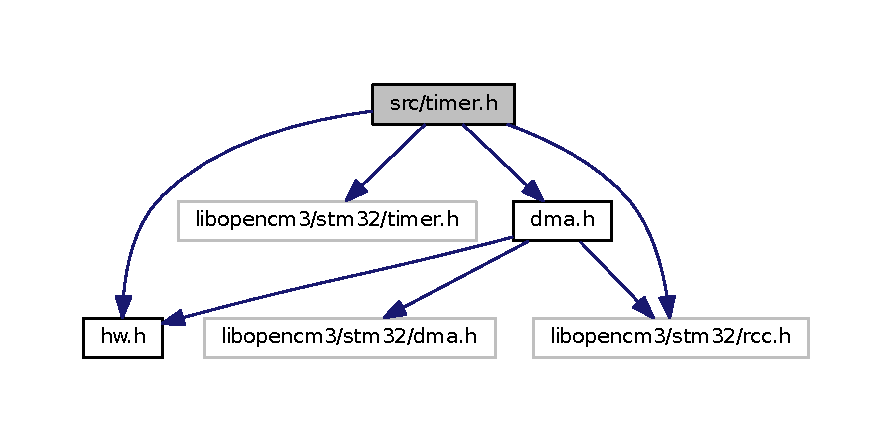
\includegraphics[width=350pt]{timer_8h__incl}
\end{center}
\end{figure}
This graph shows which files directly or indirectly include this file\+:\nopagebreak
\begin{figure}[H]
\begin{center}
\leavevmode
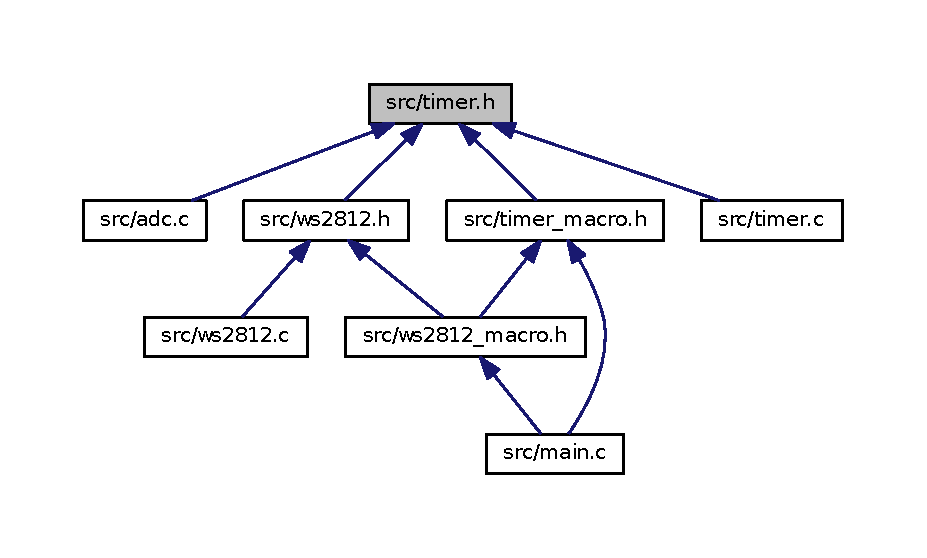
\includegraphics[width=350pt]{timer_8h__dep__incl}
\end{center}
\end{figure}
\subsection*{Classes}
\begin{DoxyCompactItemize}
\item 
struct \hyperlink{structtimer__ccr__config}{timer\+\_\+ccr\+\_\+config}
\item 
struct \hyperlink{structtimer__ccr}{timer\+\_\+ccr}
\item 
struct \hyperlink{structtimer__config}{timer\+\_\+config}
\item 
struct \hyperlink{structtimer}{timer}
\end{DoxyCompactItemize}
\subsection*{Functions}
\begin{DoxyCompactItemize}
\item 
void \hyperlink{timer_8h_a995539ac62815c22bad2313f304865b5}{timer\+\_\+ccr\+\_\+init} (struct \hyperlink{structtimer__ccr}{timer\+\_\+ccr} $\ast$ccr, enum \hyperlink{hw_8h_a3c02952100e7d051b77cdf060ca0ba9b}{hw\+\_\+init\+\_\+state} state)
\begin{DoxyCompactList}\small\item\em Upgrade \hyperlink{structtimer__ccr}{timer\+\_\+ccr} state and init hardware. \end{DoxyCompactList}\item 
void \hyperlink{timer_8h_a1e33eb6cb5bd4bd99416edbb25790760}{timer\+\_\+init} (struct \hyperlink{structtimer}{timer} $\ast$\hyperlink{structtimer}{timer}, enum \hyperlink{hw_8h_a3c02952100e7d051b77cdf060ca0ba9b}{hw\+\_\+init\+\_\+state} state)
\begin{DoxyCompactList}\small\item\em Upgrade timer\+\_\+init state and init hardware. \end{DoxyCompactList}\item 
void \hyperlink{timer_8h_a734417848b07d1d04bca5e224f13e319}{timer\+\_\+ccr\+\_\+set} (struct \hyperlink{structtimer__ccr}{timer\+\_\+ccr} $\ast$ccr, uint32\+\_\+t value)
\begin{DoxyCompactList}\small\item\em Set C\+C\+R value of \hyperlink{structtimer__ccr}{timer\+\_\+ccr}. \end{DoxyCompactList}\end{DoxyCompactItemize}


\subsection{Detailed Description}
Timer H\+A\+L include file. 



\subsection{Function Documentation}
\hypertarget{timer_8h_a995539ac62815c22bad2313f304865b5}{}\index{timer.\+h@{timer.\+h}!timer\+\_\+ccr\+\_\+init@{timer\+\_\+ccr\+\_\+init}}
\index{timer\+\_\+ccr\+\_\+init@{timer\+\_\+ccr\+\_\+init}!timer.\+h@{timer.\+h}}
\subsubsection[{timer\+\_\+ccr\+\_\+init}]{\setlength{\rightskip}{0pt plus 5cm}void timer\+\_\+ccr\+\_\+init (
\begin{DoxyParamCaption}
\item[{struct {\bf timer\+\_\+ccr} $\ast$}]{ccr, }
\item[{enum {\bf hw\+\_\+init\+\_\+state}}]{state}
\end{DoxyParamCaption}
)}\label{timer_8h_a995539ac62815c22bad2313f304865b5}


Upgrade \hyperlink{structtimer__ccr}{timer\+\_\+ccr} state and init hardware. 

\begin{DoxyRefDesc}{Todo}
\item[\hyperlink{todo__todo000006}{Todo}]Add more C\+C\+R-\/channels \end{DoxyRefDesc}


\begin{DoxyRefDesc}{Todo}
\item[\hyperlink{todo__todo000007}{Todo}]Only upgrade state if needed \end{DoxyRefDesc}


Definition at line 12 of file timer.\+c.



References D\+E\+F\+A\+U\+L\+T, H\+W\+\_\+\+I\+N\+I\+T\+\_\+\+P\+R\+E\+\_\+\+N\+V\+I\+C, H\+W\+\_\+\+I\+N\+I\+T\+\_\+\+R\+C\+C, and timer\+\_\+init().



Referenced by ws2812\+\_\+init().

\hypertarget{timer_8h_a734417848b07d1d04bca5e224f13e319}{}\index{timer.\+h@{timer.\+h}!timer\+\_\+ccr\+\_\+set@{timer\+\_\+ccr\+\_\+set}}
\index{timer\+\_\+ccr\+\_\+set@{timer\+\_\+ccr\+\_\+set}!timer.\+h@{timer.\+h}}
\subsubsection[{timer\+\_\+ccr\+\_\+set}]{\setlength{\rightskip}{0pt plus 5cm}void timer\+\_\+ccr\+\_\+set (
\begin{DoxyParamCaption}
\item[{struct {\bf timer\+\_\+ccr} $\ast$}]{ccr, }
\item[{uint32\+\_\+t}]{value}
\end{DoxyParamCaption}
)}\label{timer_8h_a734417848b07d1d04bca5e224f13e319}


Set C\+C\+R value of \hyperlink{structtimer__ccr}{timer\+\_\+ccr}. 



Definition at line 79 of file timer.\+c.

\hypertarget{timer_8h_a1e33eb6cb5bd4bd99416edbb25790760}{}\index{timer.\+h@{timer.\+h}!timer\+\_\+init@{timer\+\_\+init}}
\index{timer\+\_\+init@{timer\+\_\+init}!timer.\+h@{timer.\+h}}
\subsubsection[{timer\+\_\+init}]{\setlength{\rightskip}{0pt plus 5cm}void timer\+\_\+init (
\begin{DoxyParamCaption}
\item[{struct {\bf timer} $\ast$}]{timer, }
\item[{enum {\bf hw\+\_\+init\+\_\+state}}]{state}
\end{DoxyParamCaption}
)}\label{timer_8h_a1e33eb6cb5bd4bd99416edbb25790760}


Upgrade timer\+\_\+init state and init hardware. 



Definition at line 84 of file timer.\+c.



References H\+W\+\_\+\+I\+N\+I\+T\+\_\+\+P\+O\+S\+T\+\_\+\+I\+N\+I\+T, H\+W\+\_\+\+I\+N\+I\+T\+\_\+\+P\+R\+E\+\_\+\+N\+V\+I\+C, and H\+W\+\_\+\+I\+N\+I\+T\+\_\+\+R\+C\+C.



Referenced by timer\+\_\+ccr\+\_\+init().


\hypertarget{timer__macro_8h}{}\section{src/timer\+\_\+macro.h File Reference}
\label{timer__macro_8h}\index{src/timer\+\_\+macro.\+h@{src/timer\+\_\+macro.\+h}}


Utility macros for timers.  


{\ttfamily \#include \char`\"{}timer.\+h\char`\"{}}\\*
Include dependency graph for timer\+\_\+macro.\+h\+:
\nopagebreak
\begin{figure}[H]
\begin{center}
\leavevmode
\includegraphics[width=350pt]{timer__macro_8h__incl}
\end{center}
\end{figure}
This graph shows which files directly or indirectly include this file\+:\nopagebreak
\begin{figure}[H]
\begin{center}
\leavevmode
\includegraphics[width=233pt]{timer__macro_8h__dep__incl}
\end{center}
\end{figure}
\subsection*{Macros}
\begin{DoxyCompactItemize}
\item 
\#define {\bfseries T\+I\+M\+E\+R\+\_\+\+I\+N\+S\+T\+A\+N\+C\+E}(Name,  Timer,  Rcc,  Period)
\item 
\#define {\bfseries T\+I\+M\+E\+R\+\_\+\+C\+C\+R\+\_\+\+I\+N\+S\+T\+A\+N\+C\+E}(Name,  Timer,  Channel,  Dma,  Start\+C\+C\+R)
\item 
\hypertarget{timer__macro_8h_a3279bcf4092c38d74426dae48169f4f0}{}\#define {\bfseries T\+I\+M\+E\+R\+\_\+\+N\+O\+C\+O\+N\+F}(Name,  Timer,  Rcc)~T\+I\+M\+E\+R\+\_\+\+I\+N\+S\+T\+A\+N\+C\+E(Name, Timer, Rcc, 0)\label{timer__macro_8h_a3279bcf4092c38d74426dae48169f4f0}

\item 
\hypertarget{timer__macro_8h_a882cfce62e6e6f7f3b0cbef9e2853d8a}{}\#define {\bfseries T\+I\+M\+E\+R\+\_\+\+C\+C\+R\+\_\+\+N\+O\+C\+O\+N\+F}(Name,  Timer,  Channel,  Dma)~T\+I\+M\+E\+R\+\_\+\+C\+C\+R\+\_\+\+I\+N\+S\+T\+A\+N\+C\+E(Name, Timer, Channel, Dma, 0)\label{timer__macro_8h_a882cfce62e6e6f7f3b0cbef9e2853d8a}

\item 
\hypertarget{timer__macro_8h_afcf9e00e37f249ee79898999ba9b79c7}{}\#define {\bfseries \+\_\+\+T\+I\+M\+E\+R\+\_\+\+M\+A\+C\+R\+O\+\_\+\+H\+\_\+}\label{timer__macro_8h_afcf9e00e37f249ee79898999ba9b79c7}

\end{DoxyCompactItemize}


\subsection{Detailed Description}
Utility macros for timers. 



\subsection{Macro Definition Documentation}
\hypertarget{timer__macro_8h_aaffa297931f23f6b1d6acc68de84ba4b}{}\index{timer\+\_\+macro.\+h@{timer\+\_\+macro.\+h}!T\+I\+M\+E\+R\+\_\+\+C\+C\+R\+\_\+\+I\+N\+S\+T\+A\+N\+C\+E@{T\+I\+M\+E\+R\+\_\+\+C\+C\+R\+\_\+\+I\+N\+S\+T\+A\+N\+C\+E}}
\index{T\+I\+M\+E\+R\+\_\+\+C\+C\+R\+\_\+\+I\+N\+S\+T\+A\+N\+C\+E@{T\+I\+M\+E\+R\+\_\+\+C\+C\+R\+\_\+\+I\+N\+S\+T\+A\+N\+C\+E}!timer\+\_\+macro.\+h@{timer\+\_\+macro.\+h}}
\subsubsection[{T\+I\+M\+E\+R\+\_\+\+C\+C\+R\+\_\+\+I\+N\+S\+T\+A\+N\+C\+E}]{\setlength{\rightskip}{0pt plus 5cm}\#define T\+I\+M\+E\+R\+\_\+\+C\+C\+R\+\_\+\+I\+N\+S\+T\+A\+N\+C\+E(
\begin{DoxyParamCaption}
\item[{}]{Name, }
\item[{}]{Timer, }
\item[{}]{Channel, }
\item[{}]{Dma, }
\item[{}]{Start\+C\+C\+R}
\end{DoxyParamCaption}
)}\label{timer__macro_8h_aaffa297931f23f6b1d6acc68de84ba4b}
{\bfseries Value\+:}
\begin{DoxyCode}
\textcolor{keyword}{struct }\hyperlink{structtimer__ccr__config}{timer\_ccr\_config} Name##\_config = \{\(\backslash\)
        .timer = Timer,\(\backslash\)
        .channel = Channel,\(\backslash\)
        .dma = Dma,\(\backslash\)
    \};\(\backslash\)
    struct \hyperlink{structtimer__ccr}{timer\_ccr} Name = \{\(\backslash\)
        .configuration = &Name##\_config,\(\backslash\)
        .ccr = StartCCR,\(\backslash\)
    \};
\end{DoxyCode}


Definition at line 25 of file timer\+\_\+macro.\+h.

\hypertarget{timer__macro_8h_af329da461fefeb6d28239adb02a75eef}{}\index{timer\+\_\+macro.\+h@{timer\+\_\+macro.\+h}!T\+I\+M\+E\+R\+\_\+\+I\+N\+S\+T\+A\+N\+C\+E@{T\+I\+M\+E\+R\+\_\+\+I\+N\+S\+T\+A\+N\+C\+E}}
\index{T\+I\+M\+E\+R\+\_\+\+I\+N\+S\+T\+A\+N\+C\+E@{T\+I\+M\+E\+R\+\_\+\+I\+N\+S\+T\+A\+N\+C\+E}!timer\+\_\+macro.\+h@{timer\+\_\+macro.\+h}}
\subsubsection[{T\+I\+M\+E\+R\+\_\+\+I\+N\+S\+T\+A\+N\+C\+E}]{\setlength{\rightskip}{0pt plus 5cm}\#define T\+I\+M\+E\+R\+\_\+\+I\+N\+S\+T\+A\+N\+C\+E(
\begin{DoxyParamCaption}
\item[{}]{Name, }
\item[{}]{Timer, }
\item[{}]{Rcc, }
\item[{}]{Period}
\end{DoxyParamCaption}
)}\label{timer__macro_8h_af329da461fefeb6d28239adb02a75eef}
{\bfseries Value\+:}
\begin{DoxyCode}
\textcolor{keyword}{struct }\hyperlink{structtimer__config}{timer\_config} Name##\_config = \{\(\backslash\)
        .timer = Timer,\(\backslash\)
        .rcc = Rcc,\(\backslash\)
    \};\(\backslash\)
    \(\backslash\)
    struct \hyperlink{structtimer}{timer} Name = \{\(\backslash\)
        .configuration = &Name##\_config,\(\backslash\)
        .auto\_reload = Period,\(\backslash\)
    \};
\end{DoxyCode}


Definition at line 11 of file timer\+\_\+macro.\+h.


\hypertarget{uart_8h}{}\section{src/uart.h File Reference}
\label{uart_8h}\index{src/uart.\+h@{src/uart.\+h}}


U\+A\+R\+T H\+A\+L Include file.  


{\ttfamily \#include \char`\"{}gpio.\+h\char`\"{}}\\*
{\ttfamily \#include \char`\"{}time.\+h\char`\"{}}\\*
{\ttfamily \#include $<$libopencm3/stm32/usart.\+h$>$}\\*
Include dependency graph for uart.\+h\+:\nopagebreak
\begin{figure}[H]
\begin{center}
\leavevmode
\includegraphics[width=350pt]{uart_8h__incl}
\end{center}
\end{figure}
This graph shows which files directly or indirectly include this file\+:\nopagebreak
\begin{figure}[H]
\begin{center}
\leavevmode
\includegraphics[width=270pt]{uart_8h__dep__incl}
\end{center}
\end{figure}
\subsection*{Classes}
\begin{DoxyCompactItemize}
\item 
struct \hyperlink{structusart__config}{usart\+\_\+config}
\begin{DoxyCompactList}\small\item\em Usart configuration. \end{DoxyCompactList}\item 
struct \hyperlink{structusart}{usart}
\begin{DoxyCompactList}\small\item\em Usart. \end{DoxyCompactList}\end{DoxyCompactItemize}
\subsection*{Macros}
\begin{DoxyCompactItemize}
\item 
\#define \hyperlink{uart_8h_a9b89b39092dbeafe93f42b15700ea1b0}{usart\+\_\+blocking\+\_\+str}(uart,  str)~\hyperlink{usart_8c_aeeebc4a9b5040f2c423773a4eea7a325}{usart\+\_\+blocking\+\_\+send}(uart, str, sizeof(str)-\/1)
\begin{DoxyCompactList}\small\item\em Send string literal using blocking/polling (no dma or irq) \end{DoxyCompactList}\item 
\hypertarget{uart_8h_a7f24fb48ba75250866b828a8bc005f85}{}\#define {\bfseries \+\_\+\+U\+A\+R\+T\+\_\+\+H\+\_\+}\label{uart_8h_a7f24fb48ba75250866b828a8bc005f85}

\end{DoxyCompactItemize}
\subsection*{Functions}
\begin{DoxyCompactItemize}
\item 
void \hyperlink{uart_8h_a0e3103fc345dfb09aa255989c86805e8}{usart\+\_\+init} (struct \hyperlink{structusart}{usart} $\ast$\hyperlink{structusart}{usart}, enum \hyperlink{hw_8h_a3c02952100e7d051b77cdf060ca0ba9b}{hw\+\_\+init\+\_\+state} state)
\begin{DoxyCompactList}\small\item\em Init usart device. \end{DoxyCompactList}\item 
void \hyperlink{uart_8h_aeeebc4a9b5040f2c423773a4eea7a325}{usart\+\_\+blocking\+\_\+send} (struct \hyperlink{structusart}{usart} $\ast$\hyperlink{structusart}{usart}, volatile void $\ast$data, int length)
\begin{DoxyCompactList}\small\item\em Send data using blocking/polling method (no I\+R\+Q nor D\+M\+A) \end{DoxyCompactList}\item 
void \hyperlink{uart_8h_af3f4d75d88bd6796e15f0e756525ac2e}{usart\+\_\+blocking\+\_\+float} (struct \hyperlink{structusart}{usart} $\ast$\hyperlink{structusart}{usart}, float data)
\begin{DoxyCompactList}\small\item\em Send a formatted float using blocking/polling method (no I\+R\+Q nor D\+M\+A) \end{DoxyCompactList}\item 
void \hyperlink{uart_8h_a3af22e4da85d1cc56e9635c288cfee98}{usart\+\_\+blocking\+\_\+int} (struct \hyperlink{structusart}{usart} $\ast$\hyperlink{structusart}{usart}, int data)
\begin{DoxyCompactList}\small\item\em Send formatted integer using blocking/polling method (no I\+R\+Q nor D\+M\+A) \end{DoxyCompactList}\item 
void \hyperlink{uart_8h_ab51e225534a49a351524b2b5f26707b5}{usart\+\_\+blocking\+\_\+int\+\_\+zp} (struct \hyperlink{structusart}{usart} $\ast$\hyperlink{structusart}{usart}, int data, int dp)
\begin{DoxyCompactList}\small\item\em Send a formatted int with zeropadding using blocking/polling method (no I\+R\+Q nor D\+M\+A) \end{DoxyCompactList}\item 
void \hyperlink{uart_8h_a01c4691720757b4c3f21d6c277417459}{usart\+\_\+blocking\+\_\+strz} (struct \hyperlink{structusart}{usart} $\ast$\hyperlink{structusart}{usart}, volatile char $\ast$data)
\begin{DoxyCompactList}\small\item\em Send zero terminated string using blocking/polling method (no I\+R\+Q nor D\+M\+A) \end{DoxyCompactList}\item 
void \hyperlink{uart_8h_ab8505b37986de5265d35fdaa3569b9af}{usart\+\_\+blocking\+\_\+tm} (struct \hyperlink{structusart}{usart} $\ast$\hyperlink{structusart}{usart}, struct \hyperlink{structsw__timer__system__time}{sw\+\_\+timer\+\_\+system\+\_\+time} $\ast$\hyperlink{structtm}{tm})
\begin{DoxyCompactList}\small\item\em Send broken down time using blocking/polling (no dma/irq) \end{DoxyCompactList}\end{DoxyCompactItemize}


\subsection{Detailed Description}
U\+A\+R\+T H\+A\+L Include file. 



\subsection{Macro Definition Documentation}
\hypertarget{uart_8h_a9b89b39092dbeafe93f42b15700ea1b0}{}\index{uart.\+h@{uart.\+h}!usart\+\_\+blocking\+\_\+str@{usart\+\_\+blocking\+\_\+str}}
\index{usart\+\_\+blocking\+\_\+str@{usart\+\_\+blocking\+\_\+str}!uart.\+h@{uart.\+h}}
\subsubsection[{usart\+\_\+blocking\+\_\+str}]{\setlength{\rightskip}{0pt plus 5cm}\#define usart\+\_\+blocking\+\_\+str(
\begin{DoxyParamCaption}
\item[{}]{uart, }
\item[{}]{str}
\end{DoxyParamCaption}
)~{\bf usart\+\_\+blocking\+\_\+send}(uart, str, sizeof(str)-\/1)}\label{uart_8h_a9b89b39092dbeafe93f42b15700ea1b0}


Send string literal using blocking/polling (no dma or irq) 



Definition at line 11 of file uart.\+h.



Referenced by main(), and usart\+\_\+blocking\+\_\+tm().



\subsection{Function Documentation}
\hypertarget{uart_8h_af3f4d75d88bd6796e15f0e756525ac2e}{}\index{uart.\+h@{uart.\+h}!usart\+\_\+blocking\+\_\+float@{usart\+\_\+blocking\+\_\+float}}
\index{usart\+\_\+blocking\+\_\+float@{usart\+\_\+blocking\+\_\+float}!uart.\+h@{uart.\+h}}
\subsubsection[{usart\+\_\+blocking\+\_\+float}]{\setlength{\rightskip}{0pt plus 5cm}void usart\+\_\+blocking\+\_\+float (
\begin{DoxyParamCaption}
\item[{struct {\bf usart} $\ast$}]{usart, }
\item[{float}]{data}
\end{DoxyParamCaption}
)}\label{uart_8h_af3f4d75d88bd6796e15f0e756525ac2e}


Send a formatted float using blocking/polling method (no I\+R\+Q nor D\+M\+A) 


\begin{DoxyParams}{Parameters}
{\em usart} & Pointer to U\+S\+A\+R\+T device \\
\hline
{\em data} & Floating point value to format and send \\
\hline
\end{DoxyParams}


Definition at line 137 of file usart.\+c.



References usart\+\_\+blocking\+\_\+int(), and usart\+\_\+blocking\+\_\+int\+\_\+zp().

\hypertarget{uart_8h_a3af22e4da85d1cc56e9635c288cfee98}{}\index{uart.\+h@{uart.\+h}!usart\+\_\+blocking\+\_\+int@{usart\+\_\+blocking\+\_\+int}}
\index{usart\+\_\+blocking\+\_\+int@{usart\+\_\+blocking\+\_\+int}!uart.\+h@{uart.\+h}}
\subsubsection[{usart\+\_\+blocking\+\_\+int}]{\setlength{\rightskip}{0pt plus 5cm}void usart\+\_\+blocking\+\_\+int (
\begin{DoxyParamCaption}
\item[{struct {\bf usart} $\ast$}]{usart, }
\item[{int}]{data}
\end{DoxyParamCaption}
)}\label{uart_8h_a3af22e4da85d1cc56e9635c288cfee98}


Send formatted integer using blocking/polling method (no I\+R\+Q nor D\+M\+A) 



Definition at line 90 of file usart.\+c.



Referenced by usart\+\_\+blocking\+\_\+float(), and usart\+\_\+blocking\+\_\+tm().

\hypertarget{uart_8h_ab51e225534a49a351524b2b5f26707b5}{}\index{uart.\+h@{uart.\+h}!usart\+\_\+blocking\+\_\+int\+\_\+zp@{usart\+\_\+blocking\+\_\+int\+\_\+zp}}
\index{usart\+\_\+blocking\+\_\+int\+\_\+zp@{usart\+\_\+blocking\+\_\+int\+\_\+zp}!uart.\+h@{uart.\+h}}
\subsubsection[{usart\+\_\+blocking\+\_\+int\+\_\+zp}]{\setlength{\rightskip}{0pt plus 5cm}void usart\+\_\+blocking\+\_\+int\+\_\+zp (
\begin{DoxyParamCaption}
\item[{struct {\bf usart} $\ast$}]{usart, }
\item[{int}]{data, }
\item[{int}]{dp}
\end{DoxyParamCaption}
)}\label{uart_8h_ab51e225534a49a351524b2b5f26707b5}


Send a formatted int with zeropadding using blocking/polling method (no I\+R\+Q nor D\+M\+A) 


\begin{DoxyParams}{Parameters}
{\em usart} & Pointer to U\+S\+A\+R\+T device \\
\hline
{\em data} & Integer value to format and send \\
\hline
{\em dp} & Number of digits to use \\
\hline
\end{DoxyParams}
pow() takes like 4kb of flash so avoid it here since we are just working with integers anyway 

Definition at line 114 of file usart.\+c.



Referenced by usart\+\_\+blocking\+\_\+float(), and usart\+\_\+blocking\+\_\+tm().

\hypertarget{uart_8h_aeeebc4a9b5040f2c423773a4eea7a325}{}\index{uart.\+h@{uart.\+h}!usart\+\_\+blocking\+\_\+send@{usart\+\_\+blocking\+\_\+send}}
\index{usart\+\_\+blocking\+\_\+send@{usart\+\_\+blocking\+\_\+send}!uart.\+h@{uart.\+h}}
\subsubsection[{usart\+\_\+blocking\+\_\+send}]{\setlength{\rightskip}{0pt plus 5cm}void usart\+\_\+blocking\+\_\+send (
\begin{DoxyParamCaption}
\item[{struct {\bf usart} $\ast$}]{usart, }
\item[{volatile void $\ast$}]{data, }
\item[{int}]{length}
\end{DoxyParamCaption}
)}\label{uart_8h_aeeebc4a9b5040f2c423773a4eea7a325}


Send data using blocking/polling method (no I\+R\+Q nor D\+M\+A) 



Definition at line 71 of file usart.\+c.

\hypertarget{uart_8h_a01c4691720757b4c3f21d6c277417459}{}\index{uart.\+h@{uart.\+h}!usart\+\_\+blocking\+\_\+strz@{usart\+\_\+blocking\+\_\+strz}}
\index{usart\+\_\+blocking\+\_\+strz@{usart\+\_\+blocking\+\_\+strz}!uart.\+h@{uart.\+h}}
\subsubsection[{usart\+\_\+blocking\+\_\+strz}]{\setlength{\rightskip}{0pt plus 5cm}void usart\+\_\+blocking\+\_\+strz (
\begin{DoxyParamCaption}
\item[{struct {\bf usart} $\ast$}]{usart, }
\item[{volatile char $\ast$}]{data}
\end{DoxyParamCaption}
)}\label{uart_8h_a01c4691720757b4c3f21d6c277417459}


Send zero terminated string using blocking/polling method (no I\+R\+Q nor D\+M\+A) 



Definition at line 82 of file usart.\+c.

\hypertarget{uart_8h_ab8505b37986de5265d35fdaa3569b9af}{}\index{uart.\+h@{uart.\+h}!usart\+\_\+blocking\+\_\+tm@{usart\+\_\+blocking\+\_\+tm}}
\index{usart\+\_\+blocking\+\_\+tm@{usart\+\_\+blocking\+\_\+tm}!uart.\+h@{uart.\+h}}
\subsubsection[{usart\+\_\+blocking\+\_\+tm}]{\setlength{\rightskip}{0pt plus 5cm}void usart\+\_\+blocking\+\_\+tm (
\begin{DoxyParamCaption}
\item[{struct {\bf usart} $\ast$}]{usart, }
\item[{struct {\bf sw\+\_\+timer\+\_\+system\+\_\+time} $\ast$}]{tm}
\end{DoxyParamCaption}
)}\label{uart_8h_ab8505b37986de5265d35fdaa3569b9af}


Send broken down time using blocking/polling (no dma/irq) 



Definition at line 146 of file usart.\+c.



References sw\+\_\+timer\+\_\+system\+\_\+time\+::epoch, sw\+\_\+timer\+\_\+system\+\_\+time\+::ms, time\+\_\+tm\+\_\+from\+\_\+epoch(), tm\+::tm\+\_\+hour, tm\+::tm\+\_\+mday, tm\+::tm\+\_\+min, tm\+::tm\+\_\+mon, tm\+::tm\+\_\+sec, tm\+::tm\+\_\+year, usart\+\_\+blocking\+\_\+int(), usart\+\_\+blocking\+\_\+int\+\_\+zp(), and usart\+\_\+blocking\+\_\+str.



Referenced by main().

\hypertarget{uart_8h_a0e3103fc345dfb09aa255989c86805e8}{}\index{uart.\+h@{uart.\+h}!usart\+\_\+init@{usart\+\_\+init}}
\index{usart\+\_\+init@{usart\+\_\+init}!uart.\+h@{uart.\+h}}
\subsubsection[{usart\+\_\+init}]{\setlength{\rightskip}{0pt plus 5cm}void usart\+\_\+init (
\begin{DoxyParamCaption}
\item[{struct {\bf usart} $\ast$}]{usart, }
\item[{enum {\bf hw\+\_\+init\+\_\+state}}]{state}
\end{DoxyParamCaption}
)}\label{uart_8h_a0e3103fc345dfb09aa255989c86805e8}


Init usart device. 

\begin{DoxyRefDesc}{Todo}
\item[\hyperlink{todo__todo000008}{Todo}]Check if we are inited already \end{DoxyRefDesc}


Definition at line 38 of file usart.\+c.



References H\+W\+\_\+\+I\+N\+I\+T\+\_\+\+P\+O\+S\+T\+\_\+\+I\+N\+I\+T, H\+W\+\_\+\+I\+N\+I\+T\+\_\+\+P\+R\+E\+\_\+\+N\+V\+I\+C, H\+W\+\_\+\+I\+N\+I\+T\+\_\+\+R\+C\+C, usart\+\_\+configure\+\_\+gpio(), and usart\+\_\+set\+\_\+defaults().



Referenced by hw\+\_\+init\+\_\+state().


\hypertarget{usart_8c}{}\section{src/usart.c File Reference}
\label{usart_8c}\index{src/usart.\+c@{src/usart.\+c}}


U\+S\+A\+R\+T H\+A\+L driver.  


{\ttfamily \#include \char`\"{}uart.\+h\char`\"{}}\\*
{\ttfamily \#include $<$math.\+h$>$}\\*
Include dependency graph for usart.\+c\+:
\nopagebreak
\begin{figure}[H]
\begin{center}
\leavevmode
\includegraphics[width=350pt]{usart_8c__incl}
\end{center}
\end{figure}
\subsection*{Functions}
\begin{DoxyCompactItemize}
\item 
void \hyperlink{usart_8c_a6c89d4ecfd052df4b706797c6b35ee9a}{usart\+\_\+set\+\_\+defaults} (struct \hyperlink{structusart}{usart} $\ast$\hyperlink{structusart}{usart})
\begin{DoxyCompactList}\small\item\em Configure U\+S\+A\+R\+T to default values. \end{DoxyCompactList}\item 
void \hyperlink{usart_8c_abd17fc525b9c36f671bedf0729741976}{usart\+\_\+configure\+\_\+gpio} (struct \hyperlink{structusart}{usart} $\ast$\hyperlink{structusart}{usart})
\begin{DoxyCompactList}\small\item\em Configure U\+S\+A\+R\+T G\+P\+I\+O default values. \end{DoxyCompactList}\item 
void \hyperlink{usart_8c_a0e3103fc345dfb09aa255989c86805e8}{usart\+\_\+init} (struct \hyperlink{structusart}{usart} $\ast$\hyperlink{structusart}{usart}, enum \hyperlink{hw_8h_a3c02952100e7d051b77cdf060ca0ba9b}{hw\+\_\+init\+\_\+state} state)
\begin{DoxyCompactList}\small\item\em Init usart device. \end{DoxyCompactList}\item 
void \hyperlink{usart_8c_aeeebc4a9b5040f2c423773a4eea7a325}{usart\+\_\+blocking\+\_\+send} (struct \hyperlink{structusart}{usart} $\ast$\hyperlink{structusart}{usart}, volatile void $\ast$data, int length)
\begin{DoxyCompactList}\small\item\em Send data using blocking/polling method (no I\+R\+Q nor D\+M\+A) \end{DoxyCompactList}\item 
void \hyperlink{usart_8c_ad39a26176dc8964ea1999629b1fd71f3}{usart\+\_\+blocking\+\_\+strz} (struct \hyperlink{structusart}{usart} $\ast$\hyperlink{structusart}{usart}, volatile char $\ast$ptr)
\begin{DoxyCompactList}\small\item\em Send zero terminated string using blocking/polling method (no I\+R\+Q nor D\+M\+A) \end{DoxyCompactList}\item 
void \hyperlink{usart_8c_a3af22e4da85d1cc56e9635c288cfee98}{usart\+\_\+blocking\+\_\+int} (struct \hyperlink{structusart}{usart} $\ast$\hyperlink{structusart}{usart}, int data)
\begin{DoxyCompactList}\small\item\em Send formatted integer using blocking/polling method (no I\+R\+Q nor D\+M\+A) \end{DoxyCompactList}\item 
void \hyperlink{usart_8c_ab51e225534a49a351524b2b5f26707b5}{usart\+\_\+blocking\+\_\+int\+\_\+zp} (struct \hyperlink{structusart}{usart} $\ast$\hyperlink{structusart}{usart}, int data, int dp)
\begin{DoxyCompactList}\small\item\em Send a formatted int with zeropadding using blocking/polling method (no I\+R\+Q nor D\+M\+A) \end{DoxyCompactList}\item 
void \hyperlink{usart_8c_af3f4d75d88bd6796e15f0e756525ac2e}{usart\+\_\+blocking\+\_\+float} (struct \hyperlink{structusart}{usart} $\ast$\hyperlink{structusart}{usart}, float data)
\begin{DoxyCompactList}\small\item\em Send a formatted float using blocking/polling method (no I\+R\+Q nor D\+M\+A) \end{DoxyCompactList}\item 
void \hyperlink{usart_8c_ab8505b37986de5265d35fdaa3569b9af}{usart\+\_\+blocking\+\_\+tm} (struct \hyperlink{structusart}{usart} $\ast$\hyperlink{structusart}{usart}, struct \hyperlink{structsw__timer__system__time}{sw\+\_\+timer\+\_\+system\+\_\+time} $\ast$\hyperlink{structtm}{tm})
\begin{DoxyCompactList}\small\item\em Send broken down time using blocking/polling (no dma/irq) \end{DoxyCompactList}\end{DoxyCompactItemize}


\subsection{Detailed Description}
U\+S\+A\+R\+T H\+A\+L driver. 



\subsection{Function Documentation}
\hypertarget{usart_8c_af3f4d75d88bd6796e15f0e756525ac2e}{}\index{usart.\+c@{usart.\+c}!usart\+\_\+blocking\+\_\+float@{usart\+\_\+blocking\+\_\+float}}
\index{usart\+\_\+blocking\+\_\+float@{usart\+\_\+blocking\+\_\+float}!usart.\+c@{usart.\+c}}
\subsubsection[{usart\+\_\+blocking\+\_\+float}]{\setlength{\rightskip}{0pt plus 5cm}void usart\+\_\+blocking\+\_\+float (
\begin{DoxyParamCaption}
\item[{struct {\bf usart} $\ast$}]{usart, }
\item[{float}]{data}
\end{DoxyParamCaption}
)}\label{usart_8c_af3f4d75d88bd6796e15f0e756525ac2e}


Send a formatted float using blocking/polling method (no I\+R\+Q nor D\+M\+A) 


\begin{DoxyParams}{Parameters}
{\em usart} & Pointer to U\+S\+A\+R\+T device \\
\hline
{\em data} & Floating point value to format and send \\
\hline
\end{DoxyParams}


Definition at line 131 of file usart.\+c.



References usart\+\_\+blocking\+\_\+int(), and usart\+\_\+blocking\+\_\+int\+\_\+zp().

\hypertarget{usart_8c_a3af22e4da85d1cc56e9635c288cfee98}{}\index{usart.\+c@{usart.\+c}!usart\+\_\+blocking\+\_\+int@{usart\+\_\+blocking\+\_\+int}}
\index{usart\+\_\+blocking\+\_\+int@{usart\+\_\+blocking\+\_\+int}!usart.\+c@{usart.\+c}}
\subsubsection[{usart\+\_\+blocking\+\_\+int}]{\setlength{\rightskip}{0pt plus 5cm}void usart\+\_\+blocking\+\_\+int (
\begin{DoxyParamCaption}
\item[{struct {\bf usart} $\ast$}]{usart, }
\item[{int}]{data}
\end{DoxyParamCaption}
)}\label{usart_8c_a3af22e4da85d1cc56e9635c288cfee98}


Send formatted integer using blocking/polling method (no I\+R\+Q nor D\+M\+A) 



Definition at line 90 of file usart.\+c.



Referenced by usart\+\_\+blocking\+\_\+float(), and usart\+\_\+blocking\+\_\+tm().

\hypertarget{usart_8c_ab51e225534a49a351524b2b5f26707b5}{}\index{usart.\+c@{usart.\+c}!usart\+\_\+blocking\+\_\+int\+\_\+zp@{usart\+\_\+blocking\+\_\+int\+\_\+zp}}
\index{usart\+\_\+blocking\+\_\+int\+\_\+zp@{usart\+\_\+blocking\+\_\+int\+\_\+zp}!usart.\+c@{usart.\+c}}
\subsubsection[{usart\+\_\+blocking\+\_\+int\+\_\+zp}]{\setlength{\rightskip}{0pt plus 5cm}void usart\+\_\+blocking\+\_\+int\+\_\+zp (
\begin{DoxyParamCaption}
\item[{struct {\bf usart} $\ast$}]{usart, }
\item[{int}]{data, }
\item[{int}]{dp}
\end{DoxyParamCaption}
)}\label{usart_8c_ab51e225534a49a351524b2b5f26707b5}


Send a formatted int with zeropadding using blocking/polling method (no I\+R\+Q nor D\+M\+A) 


\begin{DoxyParams}{Parameters}
{\em usart} & Pointer to U\+S\+A\+R\+T device \\
\hline
{\em data} & Integer value to format and send \\
\hline
{\em dp} & Number of digits to use \\
\hline
\end{DoxyParams}


Definition at line 114 of file usart.\+c.



Referenced by usart\+\_\+blocking\+\_\+float(), and usart\+\_\+blocking\+\_\+tm().

\hypertarget{usart_8c_aeeebc4a9b5040f2c423773a4eea7a325}{}\index{usart.\+c@{usart.\+c}!usart\+\_\+blocking\+\_\+send@{usart\+\_\+blocking\+\_\+send}}
\index{usart\+\_\+blocking\+\_\+send@{usart\+\_\+blocking\+\_\+send}!usart.\+c@{usart.\+c}}
\subsubsection[{usart\+\_\+blocking\+\_\+send}]{\setlength{\rightskip}{0pt plus 5cm}void usart\+\_\+blocking\+\_\+send (
\begin{DoxyParamCaption}
\item[{struct {\bf usart} $\ast$}]{usart, }
\item[{volatile void $\ast$}]{data, }
\item[{int}]{length}
\end{DoxyParamCaption}
)}\label{usart_8c_aeeebc4a9b5040f2c423773a4eea7a325}


Send data using blocking/polling method (no I\+R\+Q nor D\+M\+A) 



Definition at line 71 of file usart.\+c.

\hypertarget{usart_8c_ad39a26176dc8964ea1999629b1fd71f3}{}\index{usart.\+c@{usart.\+c}!usart\+\_\+blocking\+\_\+strz@{usart\+\_\+blocking\+\_\+strz}}
\index{usart\+\_\+blocking\+\_\+strz@{usart\+\_\+blocking\+\_\+strz}!usart.\+c@{usart.\+c}}
\subsubsection[{usart\+\_\+blocking\+\_\+strz}]{\setlength{\rightskip}{0pt plus 5cm}void usart\+\_\+blocking\+\_\+strz (
\begin{DoxyParamCaption}
\item[{struct {\bf usart} $\ast$}]{usart, }
\item[{volatile char $\ast$}]{ptr}
\end{DoxyParamCaption}
)}\label{usart_8c_ad39a26176dc8964ea1999629b1fd71f3}


Send zero terminated string using blocking/polling method (no I\+R\+Q nor D\+M\+A) 



Definition at line 82 of file usart.\+c.

\hypertarget{usart_8c_ab8505b37986de5265d35fdaa3569b9af}{}\index{usart.\+c@{usart.\+c}!usart\+\_\+blocking\+\_\+tm@{usart\+\_\+blocking\+\_\+tm}}
\index{usart\+\_\+blocking\+\_\+tm@{usart\+\_\+blocking\+\_\+tm}!usart.\+c@{usart.\+c}}
\subsubsection[{usart\+\_\+blocking\+\_\+tm}]{\setlength{\rightskip}{0pt plus 5cm}void usart\+\_\+blocking\+\_\+tm (
\begin{DoxyParamCaption}
\item[{struct {\bf usart} $\ast$}]{usart, }
\item[{struct {\bf sw\+\_\+timer\+\_\+system\+\_\+time} $\ast$}]{tm}
\end{DoxyParamCaption}
)}\label{usart_8c_ab8505b37986de5265d35fdaa3569b9af}


Send broken down time using blocking/polling (no dma/irq) 



Definition at line 140 of file usart.\+c.



References sw\+\_\+timer\+\_\+system\+\_\+time\+::epoch, sw\+\_\+timer\+\_\+system\+\_\+time\+::ms, time\+\_\+tm\+\_\+from\+\_\+epoch(), tm\+::tm\+\_\+hour, tm\+::tm\+\_\+mday, tm\+::tm\+\_\+min, tm\+::tm\+\_\+mon, tm\+::tm\+\_\+sec, tm\+::tm\+\_\+year, usart\+\_\+blocking\+\_\+int(), usart\+\_\+blocking\+\_\+int\+\_\+zp(), and usart\+\_\+blocking\+\_\+str.

\hypertarget{usart_8c_abd17fc525b9c36f671bedf0729741976}{}\index{usart.\+c@{usart.\+c}!usart\+\_\+configure\+\_\+gpio@{usart\+\_\+configure\+\_\+gpio}}
\index{usart\+\_\+configure\+\_\+gpio@{usart\+\_\+configure\+\_\+gpio}!usart.\+c@{usart.\+c}}
\subsubsection[{usart\+\_\+configure\+\_\+gpio}]{\setlength{\rightskip}{0pt plus 5cm}void usart\+\_\+configure\+\_\+gpio (
\begin{DoxyParamCaption}
\item[{struct {\bf usart} $\ast$}]{usart}
\end{DoxyParamCaption}
)}\label{usart_8c_abd17fc525b9c36f671bedf0729741976}


Configure U\+S\+A\+R\+T G\+P\+I\+O default values. 



Definition at line 24 of file usart.\+c.



References D\+E\+F\+A\+U\+L\+T.



Referenced by usart\+\_\+init().

\hypertarget{usart_8c_a0e3103fc345dfb09aa255989c86805e8}{}\index{usart.\+c@{usart.\+c}!usart\+\_\+init@{usart\+\_\+init}}
\index{usart\+\_\+init@{usart\+\_\+init}!usart.\+c@{usart.\+c}}
\subsubsection[{usart\+\_\+init}]{\setlength{\rightskip}{0pt plus 5cm}void usart\+\_\+init (
\begin{DoxyParamCaption}
\item[{struct {\bf usart} $\ast$}]{usart, }
\item[{enum {\bf hw\+\_\+init\+\_\+state}}]{state}
\end{DoxyParamCaption}
)}\label{usart_8c_a0e3103fc345dfb09aa255989c86805e8}


Init usart device. 

\begin{DoxyRefDesc}{Todo}
\item[\hyperlink{todo__todo000008}{Todo}]Check if we are inited already \end{DoxyRefDesc}


Definition at line 38 of file usart.\+c.



References H\+W\+\_\+\+I\+N\+I\+T\+\_\+\+P\+O\+S\+T\+\_\+\+I\+N\+I\+T, H\+W\+\_\+\+I\+N\+I\+T\+\_\+\+P\+R\+E\+\_\+\+N\+V\+I\+C, H\+W\+\_\+\+I\+N\+I\+T\+\_\+\+R\+C\+C, usart\+\_\+configure\+\_\+gpio(), and usart\+\_\+set\+\_\+defaults().



Referenced by hw\+\_\+init\+\_\+state().

\hypertarget{usart_8c_a6c89d4ecfd052df4b706797c6b35ee9a}{}\index{usart.\+c@{usart.\+c}!usart\+\_\+set\+\_\+defaults@{usart\+\_\+set\+\_\+defaults}}
\index{usart\+\_\+set\+\_\+defaults@{usart\+\_\+set\+\_\+defaults}!usart.\+c@{usart.\+c}}
\subsubsection[{usart\+\_\+set\+\_\+defaults}]{\setlength{\rightskip}{0pt plus 5cm}void usart\+\_\+set\+\_\+defaults (
\begin{DoxyParamCaption}
\item[{struct {\bf usart} $\ast$}]{usart}
\end{DoxyParamCaption}
)}\label{usart_8c_a6c89d4ecfd052df4b706797c6b35ee9a}


Configure U\+S\+A\+R\+T to default values. 



Definition at line 9 of file usart.\+c.



References D\+E\+F\+A\+U\+L\+T.



Referenced by usart\+\_\+init().


\hypertarget{usart__macro_8h}{}\section{src/usart\+\_\+macro.h File Reference}
\label{usart__macro_8h}\index{src/usart\+\_\+macro.\+h@{src/usart\+\_\+macro.\+h}}


Helper macros for U\+S\+A\+R\+T.  


{\ttfamily \#include \char`\"{}uart.\+h\char`\"{}}\\*
Include dependency graph for usart\+\_\+macro.\+h\+:\nopagebreak
\begin{figure}[H]
\begin{center}
\leavevmode
\includegraphics[width=350pt]{usart__macro_8h__incl}
\end{center}
\end{figure}
This graph shows which files directly or indirectly include this file\+:\nopagebreak
\begin{figure}[H]
\begin{center}
\leavevmode
\includegraphics[width=184pt]{usart__macro_8h__dep__incl}
\end{center}
\end{figure}
\subsection*{Macros}
\begin{DoxyCompactItemize}
\item 
\#define \hyperlink{usart__macro_8h_aecf43678b0c09f7c3c6b8a0751e9e1c9}{U\+S\+A\+R\+T\+\_\+8\+N1}(Name,  Usart,  Rcc,  Baudrate,  Rx\+\_\+pin,  Tx\+\_\+pin)
\begin{DoxyCompactList}\small\item\em Create usart, configured with 8 data bits, 1 stop bit, no parity. \end{DoxyCompactList}\item 
\hypertarget{usart__macro_8h_a16db80b3de545c6de81da706d1dd2aba}{}\#define {\bfseries \+\_\+\+U\+S\+A\+R\+T\+\_\+\+M\+A\+C\+R\+O\+\_\+\+H\+\_\+}\label{usart__macro_8h_a16db80b3de545c6de81da706d1dd2aba}

\end{DoxyCompactItemize}


\subsection{Detailed Description}
Helper macros for U\+S\+A\+R\+T. 



\subsection{Macro Definition Documentation}
\hypertarget{usart__macro_8h_aecf43678b0c09f7c3c6b8a0751e9e1c9}{}\index{usart\+\_\+macro.\+h@{usart\+\_\+macro.\+h}!U\+S\+A\+R\+T\+\_\+8\+N1@{U\+S\+A\+R\+T\+\_\+8\+N1}}
\index{U\+S\+A\+R\+T\+\_\+8\+N1@{U\+S\+A\+R\+T\+\_\+8\+N1}!usart\+\_\+macro.\+h@{usart\+\_\+macro.\+h}}
\subsubsection[{U\+S\+A\+R\+T\+\_\+8\+N1}]{\setlength{\rightskip}{0pt plus 5cm}\#define U\+S\+A\+R\+T\+\_\+8\+N1(
\begin{DoxyParamCaption}
\item[{}]{Name, }
\item[{}]{Usart, }
\item[{}]{Rcc, }
\item[{}]{Baudrate, }
\item[{}]{Rx\+\_\+pin, }
\item[{}]{Tx\+\_\+pin}
\end{DoxyParamCaption}
)}\label{usart__macro_8h_aecf43678b0c09f7c3c6b8a0751e9e1c9}
{\bfseries Value\+:}
\begin{DoxyCode}
\(\backslash\)
    struct \hyperlink{structusart__config}{usart\_config} Name##\_config = \{\(\backslash\)
        .tx\_pin = Tx\_pin,\(\backslash\)
        .rx\_pin = Rx\_pin,\(\backslash\)
        .usart = Usart,\(\backslash\)
        .rcc = Rcc,\(\backslash\)
        .baudrate = Baudrate,\(\backslash\)
    \};\(\backslash\)
    \(\backslash\)
    struct \hyperlink{structusart}{usart} Serial = \{\(\backslash\)
        .configuration = &Name##\_config,\(\backslash\)
    \};
\end{DoxyCode}


Create usart, configured with 8 data bits, 1 stop bit, no parity. 



Definition at line 10 of file usart\+\_\+macro.\+h.


\hypertarget{ws2812_8c}{}\section{src/ws2812.c File Reference}
\label{ws2812_8c}\index{src/ws2812.\+c@{src/ws2812.\+c}}


Implementation of W\+S2812 H\+A\+L.  


{\ttfamily \#include \char`\"{}ws2812.\+h\char`\"{}}\\*
Include dependency graph for ws2812.\+c\+:\nopagebreak
\begin{figure}[H]
\begin{center}
\leavevmode
\includegraphics[width=350pt]{ws2812_8c__incl}
\end{center}
\end{figure}
\subsection*{Functions}
\begin{DoxyCompactItemize}
\item 
void \hyperlink{ws2812_8c_abe4c1d1365ba3b842e733f00ff5b8cb4}{ws2812\+\_\+configure\+\_\+timer} (struct \hyperlink{structws2812}{ws2812} $\ast$led)
\begin{DoxyCompactList}\small\item\em Apply default configuration to the timer. \end{DoxyCompactList}\item 
void \hyperlink{ws2812_8c_a35b250d1bf6fa32e168ca7d559309c9a}{ws2812\+\_\+configure\+\_\+gpio} (struct \hyperlink{structws2812}{ws2812} $\ast$led)
\begin{DoxyCompactList}\small\item\em Apply default configuration to G\+P\+I\+O. \end{DoxyCompactList}\item 
void \hyperlink{ws2812_8c_a077cfeecec2b7fbefaed4e75631e76c7}{ws2812\+\_\+set\+\_\+defaults} (struct \hyperlink{structws2812}{ws2812} $\ast$led)
\begin{DoxyCompactList}\small\item\em Apply default configration to \hyperlink{structws2812}{ws2812}. \end{DoxyCompactList}\item 
void \hyperlink{ws2812_8c_adbff51511c0bd9a408d6065a5c2b9851}{ws2812\+\_\+init} (struct \hyperlink{structws2812}{ws2812} $\ast$led, enum \hyperlink{hw_8h_a3c02952100e7d051b77cdf060ca0ba9b}{hw\+\_\+init\+\_\+state} state)
\begin{DoxyCompactList}\small\item\em Initiate \hyperlink{structws2812}{ws2812} bus to state. \end{DoxyCompactList}\item 
void \hyperlink{ws2812_8c_a76c614084b51bd6644076828269cecf6}{ws2812\+\_\+process\+\_\+buffer} (struct \hyperlink{structws2812}{ws2812} $\ast$led)
\begin{DoxyCompactList}\small\item\em Process L\+E\+D buffer. \end{DoxyCompactList}\item 
void \hyperlink{ws2812_8c_a4dbb8822e64ed089eb01c8145817e3ed}{ws2812\+\_\+update} (struct \hyperlink{structws2812}{ws2812} $\ast$led)
\begin{DoxyCompactList}\small\item\em Send data to L\+E\+Ds. \end{DoxyCompactList}\item 
void \hyperlink{ws2812_8c_a82f2823a0771f8d6e1671ce1078aa5db}{ws2812\+\_\+update\+\_\+blocking} (struct \hyperlink{structws2812}{ws2812} $\ast$led)
\begin{DoxyCompactList}\small\item\em Send data to L\+E\+Ds, wait for completion. \end{DoxyCompactList}\item 
void \hyperlink{ws2812_8c_a563ef0da6498fc194067eed2611705a9}{ws2812\+\_\+set\+\_\+led} (struct \hyperlink{structws2812}{ws2812} $\ast$led, int index, int r, int g, int b)
\begin{DoxyCompactList}\small\item\em Set L\+E\+D buffer index to color r, g, b (0-\/255) \end{DoxyCompactList}\end{DoxyCompactItemize}


\subsection{Detailed Description}
Implementation of W\+S2812 H\+A\+L. 



\subsection{Function Documentation}
\hypertarget{ws2812_8c_a35b250d1bf6fa32e168ca7d559309c9a}{}\index{ws2812.\+c@{ws2812.\+c}!ws2812\+\_\+configure\+\_\+gpio@{ws2812\+\_\+configure\+\_\+gpio}}
\index{ws2812\+\_\+configure\+\_\+gpio@{ws2812\+\_\+configure\+\_\+gpio}!ws2812.\+c@{ws2812.\+c}}
\subsubsection[{ws2812\+\_\+configure\+\_\+gpio}]{\setlength{\rightskip}{0pt plus 5cm}void ws2812\+\_\+configure\+\_\+gpio (
\begin{DoxyParamCaption}
\item[{struct {\bf ws2812} $\ast$}]{led}
\end{DoxyParamCaption}
)}\label{ws2812_8c_a35b250d1bf6fa32e168ca7d559309c9a}


Apply default configuration to G\+P\+I\+O. 


\begin{DoxyParams}{Parameters}
{\em led} & Bus to use \\
\hline
\end{DoxyParams}


Definition at line 22 of file ws2812.\+c.



References ws2812\+::configuration, D\+E\+F\+A\+U\+L\+T, and ws2812\+\_\+config\+::pin.



Referenced by ws2812\+\_\+init().

\hypertarget{ws2812_8c_abe4c1d1365ba3b842e733f00ff5b8cb4}{}\index{ws2812.\+c@{ws2812.\+c}!ws2812\+\_\+configure\+\_\+timer@{ws2812\+\_\+configure\+\_\+timer}}
\index{ws2812\+\_\+configure\+\_\+timer@{ws2812\+\_\+configure\+\_\+timer}!ws2812.\+c@{ws2812.\+c}}
\subsubsection[{ws2812\+\_\+configure\+\_\+timer}]{\setlength{\rightskip}{0pt plus 5cm}void ws2812\+\_\+configure\+\_\+timer (
\begin{DoxyParamCaption}
\item[{struct {\bf ws2812} $\ast$}]{led}
\end{DoxyParamCaption}
)}\label{ws2812_8c_abe4c1d1365ba3b842e733f00ff5b8cb4}


Apply default configuration to the timer. 


\begin{DoxyParams}{Parameters}
{\em led} & Bus to use \\
\hline
\end{DoxyParams}


Definition at line 15 of file ws2812.\+c.



References ws2812\+\_\+config\+::ccr, ws2812\+::configuration, D\+E\+F\+A\+U\+L\+T, and ws2812\+\_\+config\+::frequency.



Referenced by ws2812\+\_\+init().

\hypertarget{ws2812_8c_adbff51511c0bd9a408d6065a5c2b9851}{}\index{ws2812.\+c@{ws2812.\+c}!ws2812\+\_\+init@{ws2812\+\_\+init}}
\index{ws2812\+\_\+init@{ws2812\+\_\+init}!ws2812.\+c@{ws2812.\+c}}
\subsubsection[{ws2812\+\_\+init}]{\setlength{\rightskip}{0pt plus 5cm}void ws2812\+\_\+init (
\begin{DoxyParamCaption}
\item[{struct {\bf ws2812} $\ast$}]{led, }
\item[{enum {\bf hw\+\_\+init\+\_\+state}}]{state}
\end{DoxyParamCaption}
)}\label{ws2812_8c_adbff51511c0bd9a408d6065a5c2b9851}


Initiate \hyperlink{structws2812}{ws2812} bus to state. 


\begin{DoxyParams}{Parameters}
{\em led} & Bus to init \\
\hline
{\em state} & New H\+W state \\
\hline
\end{DoxyParams}


Definition at line 40 of file ws2812.\+c.



References ws2812\+\_\+config\+::ccr, ws2812\+::configuration, H\+W\+\_\+\+I\+N\+I\+T\+\_\+\+G\+P\+I\+O, H\+W\+\_\+\+I\+N\+I\+T\+\_\+\+P\+O\+S\+T\+\_\+\+I\+N\+I\+T, H\+W\+\_\+\+I\+N\+I\+T\+\_\+\+P\+R\+E\+\_\+\+N\+V\+I\+C, ws2812\+\_\+config\+::pin, timer\+\_\+ccr\+\_\+init(), ws2812\+\_\+configure\+\_\+gpio(), ws2812\+\_\+configure\+\_\+timer(), and ws2812\+\_\+set\+\_\+defaults().



Referenced by hw\+\_\+init\+\_\+state().

\hypertarget{ws2812_8c_a76c614084b51bd6644076828269cecf6}{}\index{ws2812.\+c@{ws2812.\+c}!ws2812\+\_\+process\+\_\+buffer@{ws2812\+\_\+process\+\_\+buffer}}
\index{ws2812\+\_\+process\+\_\+buffer@{ws2812\+\_\+process\+\_\+buffer}!ws2812.\+c@{ws2812.\+c}}
\subsubsection[{ws2812\+\_\+process\+\_\+buffer}]{\setlength{\rightskip}{0pt plus 5cm}void ws2812\+\_\+process\+\_\+buffer (
\begin{DoxyParamCaption}
\item[{struct {\bf ws2812} $\ast$}]{led}
\end{DoxyParamCaption}
)}\label{ws2812_8c_a76c614084b51bd6644076828269cecf6}


Process L\+E\+D buffer. 



Definition at line 65 of file ws2812.\+c.



References ws2812\+\_\+rgb\+::b, ws2812\+\_\+config\+::bit0, ws2812\+\_\+config\+::bit1, ws2812\+::configuration, ws2812\+\_\+rgb\+::g, ws2812\+::led\+\_\+buffer, ws2812\+::led\+\_\+count, ws2812\+::pwm\+\_\+buffer, and ws2812\+\_\+rgb\+::r.



Referenced by ws2812\+\_\+update(), and ws2812\+\_\+update\+\_\+blocking().

\hypertarget{ws2812_8c_a077cfeecec2b7fbefaed4e75631e76c7}{}\index{ws2812.\+c@{ws2812.\+c}!ws2812\+\_\+set\+\_\+defaults@{ws2812\+\_\+set\+\_\+defaults}}
\index{ws2812\+\_\+set\+\_\+defaults@{ws2812\+\_\+set\+\_\+defaults}!ws2812.\+c@{ws2812.\+c}}
\subsubsection[{ws2812\+\_\+set\+\_\+defaults}]{\setlength{\rightskip}{0pt plus 5cm}void ws2812\+\_\+set\+\_\+defaults (
\begin{DoxyParamCaption}
\item[{struct {\bf ws2812} $\ast$}]{led}
\end{DoxyParamCaption}
)}\label{ws2812_8c_a077cfeecec2b7fbefaed4e75631e76c7}


Apply default configration to \hyperlink{structws2812}{ws2812}. 


\begin{DoxyParams}{Parameters}
{\em led} & Bus to use \\
\hline
\end{DoxyParams}


Definition at line 30 of file ws2812.\+c.



References ws2812\+\_\+config\+::bit0, ws2812\+\_\+config\+::bit1, ws2812\+::configuration, D\+E\+F\+A\+U\+L\+T, and ws2812\+\_\+config\+::frequency.



Referenced by ws2812\+\_\+init().

\hypertarget{ws2812_8c_a563ef0da6498fc194067eed2611705a9}{}\index{ws2812.\+c@{ws2812.\+c}!ws2812\+\_\+set\+\_\+led@{ws2812\+\_\+set\+\_\+led}}
\index{ws2812\+\_\+set\+\_\+led@{ws2812\+\_\+set\+\_\+led}!ws2812.\+c@{ws2812.\+c}}
\subsubsection[{ws2812\+\_\+set\+\_\+led}]{\setlength{\rightskip}{0pt plus 5cm}void ws2812\+\_\+set\+\_\+led (
\begin{DoxyParamCaption}
\item[{struct {\bf ws2812} $\ast$}]{led, }
\item[{int}]{index, }
\item[{int}]{r, }
\item[{int}]{g, }
\item[{int}]{b}
\end{DoxyParamCaption}
)}\label{ws2812_8c_a563ef0da6498fc194067eed2611705a9}


Set L\+E\+D buffer index to color r, g, b (0-\/255) 



Definition at line 96 of file ws2812.\+c.



References ws2812\+\_\+rgb\+::g, ws2812\+::led\+\_\+buffer, and ws2812\+\_\+rgb\+::r.



Referenced by set\+\_\+status\+\_\+color().

\hypertarget{ws2812_8c_a4dbb8822e64ed089eb01c8145817e3ed}{}\index{ws2812.\+c@{ws2812.\+c}!ws2812\+\_\+update@{ws2812\+\_\+update}}
\index{ws2812\+\_\+update@{ws2812\+\_\+update}!ws2812.\+c@{ws2812.\+c}}
\subsubsection[{ws2812\+\_\+update}]{\setlength{\rightskip}{0pt plus 5cm}void ws2812\+\_\+update (
\begin{DoxyParamCaption}
\item[{struct {\bf ws2812} $\ast$}]{led}
\end{DoxyParamCaption}
)}\label{ws2812_8c_a4dbb8822e64ed089eb01c8145817e3ed}


Send data to L\+E\+Ds. 



Definition at line 80 of file ws2812.\+c.



References ws2812\+\_\+config\+::ccr, ws2812\+::configuration, ws2812\+::led\+\_\+count, ws2812\+::pwm\+\_\+buffer, and ws2812\+\_\+process\+\_\+buffer().

\hypertarget{ws2812_8c_a82f2823a0771f8d6e1671ce1078aa5db}{}\index{ws2812.\+c@{ws2812.\+c}!ws2812\+\_\+update\+\_\+blocking@{ws2812\+\_\+update\+\_\+blocking}}
\index{ws2812\+\_\+update\+\_\+blocking@{ws2812\+\_\+update\+\_\+blocking}!ws2812.\+c@{ws2812.\+c}}
\subsubsection[{ws2812\+\_\+update\+\_\+blocking}]{\setlength{\rightskip}{0pt plus 5cm}void ws2812\+\_\+update\+\_\+blocking (
\begin{DoxyParamCaption}
\item[{struct {\bf ws2812} $\ast$}]{led}
\end{DoxyParamCaption}
)}\label{ws2812_8c_a82f2823a0771f8d6e1671ce1078aa5db}


Send data to L\+E\+Ds, wait for completion. 



Definition at line 90 of file ws2812.\+c.



References ws2812\+\_\+config\+::ccr, ws2812\+::configuration, ws2812\+::led\+\_\+count, ws2812\+::pwm\+\_\+buffer, and ws2812\+\_\+process\+\_\+buffer().



Referenced by set\+\_\+status\+\_\+color().


\hypertarget{ws2812_8h}{}\section{src/ws2812.h File Reference}
\label{ws2812_8h}\index{src/ws2812.\+h@{src/ws2812.\+h}}


W\+S2812 H\+A\+L include file.  


{\ttfamily \#include \char`\"{}gpio.\+h\char`\"{}}\\*
{\ttfamily \#include \char`\"{}timer.\+h\char`\"{}}\\*
{\ttfamily \#include \char`\"{}dma.\+h\char`\"{}}\\*
Include dependency graph for ws2812.\+h\+:
\nopagebreak
\begin{figure}[H]
\begin{center}
\leavevmode
\includegraphics[width=350pt]{ws2812_8h__incl}
\end{center}
\end{figure}
This graph shows which files directly or indirectly include this file\+:\nopagebreak
\begin{figure}[H]
\begin{center}
\leavevmode
\includegraphics[width=292pt]{ws2812_8h__dep__incl}
\end{center}
\end{figure}
\subsection*{Classes}
\begin{DoxyCompactItemize}
\item 
struct \hyperlink{structws2812__config}{ws2812\+\_\+config}
\begin{DoxyCompactList}\small\item\em Configuration for W\+S2812. \end{DoxyCompactList}\item 
struct \hyperlink{structws2812}{ws2812}
\begin{DoxyCompactList}\small\item\em W\+S2812 Instance. \end{DoxyCompactList}\item 
struct \hyperlink{structws2812__rgb}{ws2812\+\_\+rgb}
\begin{DoxyCompactList}\small\item\em 24 bit color \end{DoxyCompactList}\end{DoxyCompactItemize}
\subsection*{Functions}
\begin{DoxyCompactItemize}
\item 
void \hyperlink{ws2812_8h_adbff51511c0bd9a408d6065a5c2b9851}{ws2812\+\_\+init} (struct \hyperlink{structws2812}{ws2812} $\ast$led, enum \hyperlink{hw_8h_a3c02952100e7d051b77cdf060ca0ba9b}{hw\+\_\+init\+\_\+state} state)
\begin{DoxyCompactList}\small\item\em Initiate \hyperlink{structws2812}{ws2812} bus to state. \end{DoxyCompactList}\item 
\hypertarget{ws2812_8h_a4dbb8822e64ed089eb01c8145817e3ed}{}void {\bfseries ws2812\+\_\+update} (struct \hyperlink{structws2812}{ws2812} $\ast$led)\label{ws2812_8h_a4dbb8822e64ed089eb01c8145817e3ed}

\item 
\hypertarget{ws2812_8h_a563ef0da6498fc194067eed2611705a9}{}void {\bfseries ws2812\+\_\+set\+\_\+led} (struct \hyperlink{structws2812}{ws2812} $\ast$led, int index, int r, int g, int b)\label{ws2812_8h_a563ef0da6498fc194067eed2611705a9}

\item 
\hypertarget{ws2812_8h_a82f2823a0771f8d6e1671ce1078aa5db}{}void {\bfseries ws2812\+\_\+update\+\_\+blocking} (struct \hyperlink{structws2812}{ws2812} $\ast$led)\label{ws2812_8h_a82f2823a0771f8d6e1671ce1078aa5db}

\end{DoxyCompactItemize}


\subsection{Detailed Description}
W\+S2812 H\+A\+L include file. 



\subsection{Function Documentation}
\hypertarget{ws2812_8h_adbff51511c0bd9a408d6065a5c2b9851}{}\index{ws2812.\+h@{ws2812.\+h}!ws2812\+\_\+init@{ws2812\+\_\+init}}
\index{ws2812\+\_\+init@{ws2812\+\_\+init}!ws2812.\+h@{ws2812.\+h}}
\subsubsection[{ws2812\+\_\+init}]{\setlength{\rightskip}{0pt plus 5cm}void ws2812\+\_\+init (
\begin{DoxyParamCaption}
\item[{struct {\bf ws2812} $\ast$}]{led, }
\item[{enum {\bf hw\+\_\+init\+\_\+state}}]{state}
\end{DoxyParamCaption}
)}\label{ws2812_8h_adbff51511c0bd9a408d6065a5c2b9851}


Initiate \hyperlink{structws2812}{ws2812} bus to state. 


\begin{DoxyParams}{Parameters}
{\em led} & Bus to init \\
\hline
{\em state} & New H\+W state \\
\hline
\end{DoxyParams}


Definition at line 40 of file ws2812.\+c.



References ws2812\+\_\+config\+::ccr, ws2812\+::configuration, H\+W\+\_\+\+I\+N\+I\+T\+\_\+\+G\+P\+I\+O, H\+W\+\_\+\+I\+N\+I\+T\+\_\+\+P\+O\+S\+T\+\_\+\+I\+N\+I\+T, H\+W\+\_\+\+I\+N\+I\+T\+\_\+\+P\+R\+E\+\_\+\+N\+V\+I\+C, ws2812\+\_\+config\+::pin, timer\+\_\+ccr\+\_\+init(), ws2812\+\_\+configure\+\_\+gpio(), ws2812\+\_\+configure\+\_\+timer(), and ws2812\+\_\+set\+\_\+defaults().



Referenced by hw\+\_\+init\+\_\+state().


\hypertarget{ws2812__macro_8h}{}\section{src/ws2812\+\_\+macro.h File Reference}
\label{ws2812__macro_8h}\index{src/ws2812\+\_\+macro.\+h@{src/ws2812\+\_\+macro.\+h}}


Helper macros for \hyperlink{structws2812}{ws2812}.  


{\ttfamily \#include \char`\"{}ws2812.\+h\char`\"{}}\\*
{\ttfamily \#include \char`\"{}gpio\+\_\+macro.\+h\char`\"{}}\\*
{\ttfamily \#include \char`\"{}timer\+\_\+macro.\+h\char`\"{}}\\*
Include dependency graph for ws2812\+\_\+macro.\+h\+:
\nopagebreak
\begin{figure}[H]
\begin{center}
\leavevmode
\includegraphics[width=350pt]{ws2812__macro_8h__incl}
\end{center}
\end{figure}
This graph shows which files directly or indirectly include this file\+:\nopagebreak
\begin{figure}[H]
\begin{center}
\leavevmode
\includegraphics[width=195pt]{ws2812__macro_8h__dep__incl}
\end{center}
\end{figure}


\subsection{Detailed Description}
Helper macros for \hyperlink{structws2812}{ws2812}. 


%--- End generated contents ---

% Index
\backmatter
\newpage
\phantomsection
\clearemptydoublepage
\addcontentsline{toc}{chapter}{Index}
\printindex

\end{document}
